% Plantilla realizada por Alberto Brunete (UPM). Basada en la de Santiago Morante Cendrero (UC3M)

%parametros de tipo libro
\documentclass[10pt,a4paper]{book}

%idioma espa�ol y acentos
\usepackage[latin1]{inputenc}
\usepackage[spanish, USenglish, es-tabla]{babel}

%algunos s�mbolos matem�ticos y paquete para usar subim�genes
\usepackage{amsmath}
\usepackage{amsfonts}
\usepackage{amssymb}
\usepackage{graphicx}
\usepackage{subfigure}
\usepackage{listings}
\usepackage{appendix}
\usepackage{cite}
\usepackage{url}
\usepackage{natbib}
\usepackage{pgfgantt} %para realizar diagramas de gantt
\usepackage{lscape} %para poner la pagina en horizontal
\usepackage{caption}
\usepackage{epigraph}
\usepackage{color}
\definecolor{gray97}{gray}{.97}
\definecolor{gray75}{gray}{.75}
\definecolor{gray45}{gray}{.45}

\DeclareCaptionType{code}[C�digo][�ndice de c�digos]

%para el anexo en espa�ol
\renewcommand{\appendixname}{Ap�ndice}
\renewcommand{\appendixtocname}{Ap�ndice}
\renewcommand{\appendixpagename}{Ap�ndice}

%para mostrar fragmentos de codigo fuente
\lstset{ frame=Ltb,
     framerule=0pt,
     aboveskip=0.5cm,
     framextopmargin=3pt,
     framexbottommargin=3pt,
     framexleftmargin=0.4cm,
     framesep=0pt,
     rulesep=.4pt,
     backgroundcolor=\color{gray97},
     rulesepcolor=\color{black},
     %
     stringstyle=\ttfamily,
     showstringspaces = false,
     basicstyle=\small\ttfamily,
     commentstyle=\color{gray45},
     keywordstyle=\bfseries,
     %
     numbers=left,
     numbersep=15pt,
     numberstyle=\tiny,
     numberfirstline = false,
     breaklines=true,
   }
 
% minimizar fragmentado de listados
\lstnewenvironment{listing}[1][]
   {\lstset{#1}\pagebreak[0]}{\pagebreak[0]}
 
\lstdefinestyle{consola}
   {basicstyle=\scriptsize\bf\ttfamily,
    backgroundcolor=\color{gray75},
   }
   
\lstdefinestyle{launch}
   {basicstyle=\scriptsize\bf\ttfamily,
   }
 
\lstdefinestyle{C++}
   {language=C++,
   }
   
%M�rgenes
\usepackage[left=3cm,top=3cm,right=3cm,bottom=3cm]{geometry}

%
\usepackage{multicol}
\usepackage{enumerate} % enumerados

%para generar �ndice con hiperv�nculos
\usepackage{hyperref}

%parametros del documento (sus propiedades)
\hypersetup{
    pdftitle={Manzaneque Amo, Daniel - Guiado de un robot m�vil basado en ROS y Kinect - 2016},
    pdfsubject={TFG - 2016},
    pdfauthor={Manzaneque Amo, Daniel},
    pdfkeywords={robot m�vil} {ROS} {navegci�n reactiva} {c�lculo de trayectorias},
    colorlinks,
    citecolor=brown,
    filecolor=black,
    linkcolor=black,
    urlcolor=blue,
}

%empieza el documento
\begin{document}  

%elementos antes del trabajo en s� se meten dentro de frontmatter
\frontmatter

%cada incluye referencia a un archivo de tipo .tex
\begin{titlepage}
\begin{center}

%forma de introducir im�genes. el \\[0.5 cm] de final de l�nea introduce un salto de ese tama�o.
%width=1\textwidth indica el tama�o de la im�gen (valores entre 0-1). 
 
\includegraphics[width=1\textwidth]{figuras/cabecera.png}  \\[0.5 cm]

\LARGE UNIVERSIDAD POLIT�CNICA DE MADRID \\ [1 cm]

\LARGE ESCUELA T�CNICA SUPERIOR DE INGENIER�A Y DISE�O INDUSTRIAL \\ [1 cm]

\LARGE Grado en Ingenier�a Electr�nica Industrial y Autom�tica\\ [1 cm]

\LARGE \textbf{TRABAJO FIN DE GRADO}\\[1 cm]

\Huge \textsc{Guiado de un robot m�vil basado en ROS y kinect}\\[1 cm]

\LARGE Autor: Daniel Manzaneque Amo \\[2 cm]

%flushleft alinea a la izquierda el texto

\begin{multicols}{2} 
\begin{flushleft} \Large
\emph{Cotutor:} Miguel Hernando\\
\emph{Departamento:} Electr�nica, Autom�tica e Inform�tica Industrial
\end{flushleft}

\begin{flushleft} \Large
\emph{Tutor:} Alberto Brunete\\
\emph{Departamento:} Electr�nica, Autom�tica e Inform�tica Industrial
\end{flushleft}

\end{multicols} 

%rellena de blanco el resto de la p�gina para escribir abajo del todo
\vfill

% Bottom of the page
{\large Madrid, Febrero 2016}

\end{center}
\end{titlepage}

\begin{center}

%forma de introducir im�genes. el \\[0.5 cm] de final de l�nea introduce un salto de ese tama�o.
%width=1\textwidth indica el tama�o de la im�gen (valores entre 0-1). 
 
\includegraphics[width=1\textwidth]{figuras/cabecera.png}  \\[0.5 cm]

\LARGE UNIVERSIDAD POLIT�CNICA DE MADRID \\ [1 cm]

\LARGE ESCUELA T�CNICA SUPERIOR DE INGENIER�A Y DISE�O INDUSTRIAL \\ [1 cm]

\LARGE Grado en Ingenier�a Electr�nica y Autom�tica Industrial\\ [1 cm]

\LARGE \textbf{TRABAJO FIN DE GRADO}\\[1 cm]

\Huge \textsc{Guiado de un robot m�vil basado en ROS y kinect}\\[4 cm]

\Large Firma Autor \\[3 cm]

%flushleft alinea a la izquierda el texto

\begin{multicols}{2} 
\begin{flushleft} 
\Large \emph{Firma Cotutor}
\end{flushleft}

\begin{flushright} 
\Large \emph{Firma Tutor}
\end{flushright}

\end{multicols} 

%rellena de blanco el resto de la p�gina para escribir abajo del todo
\vfill

\end{center}

%Licencia opcional
\begin{flushleft}

Copyright \copyright 2916. Daniel Manzaneque Amo

%ejemplo de licencia, se puede elegir cualquier otra

Esta obra est� licenciada bajo la licencia Creative Commons Atribuci�n-NoComercial-SinDerivadas 3.0 Unported (CC BY-NC-ND 3.0). Para ver una copia de esta licencia, visite http://creativecommons.org/licenses/by-nc-nd/3.0/deed.es o env�e una carta a Creative Commons, 444 Castro Street, Suite 900, Mountain View, California, 94041, EE.UU.

Todas las opiniones aqu� expresadas son del autor, y no reflejan necesariamente las opiniones de la Universidad Polit�cnica de Madrid.

\end{flushleft}

\cleardoublepage

\begin{flushleft} \large
\textbf{T�tulo:} Guiado de un robot m�vil basado en ROS y kinect \\
\textbf{Autor:} Daniel Manzaneque Amo\\
\textbf{Tutor:} Dr. Alberto Brunete Gonz�lez\\ 
\textbf{Cotutor:} Dr. Miguel Hernando Guti�rrez\\ [1 cm]

\end{flushleft} 

\begin{center} \LARGE
EL TRIBUNAL \\ [1 cm]
\end{center}

\begin{flushleft} \LARGE
Presidente: \\ [1 cm]
Vocal: \\ [1 cm]
Secretario: \\ [1.5 cm]
\end{flushleft}

\large
Realizado el acto de defensa y lectura del Trabajo Fin de Grado el d�a ....... de ....................   de ... en .........., en la Escuela T�cnica Superior de Ingenier�a y Dise�o Industrial de la Universidad Polit�cnica de Madrid, acuerda otorgarle la CALIFICACI�N de: \\ [2 cm]

\begin{center}
 \large VOCAL \\ [2.2 cm]
\end{center}

\begin{minipage}{0.5\textwidth}
 \begin{flushleft}
 \large SECRETARIO
\end{flushleft}
\end{minipage}
\begin{minipage}{0.5\textwidth}
\begin{flushright}
 \large PRESIDENTE
\end{flushright} 
\end{minipage}
%espaciado entre parrafos 8mm mayor del habitual
\setlength{\parskip}{4mm}

\thispagestyle{empty}
\null\vfill

\cleardoublepage

\begin{flushright}
\parbox{8cm}{
  \raggedright{\large\itshape
   A man ought to read \\ 
  just as his inclination leads him; \\
  for what he reads as a task \\ 
  will do him little good.\par\bigskip
  }   
  \raggedleft{--- \textup{Vetusta Morla}, Los Buenos}\par
}
\end{flushright}

\vfill\vfill

\clearpage







%\epigraphfontsize{\small\itshape}
%\setlength{\epigraphwidth}{.6\textwidth}
%\begin{epigraphs}
%\qitem{``Lo s\'{e} porque muchos ya se fueron y hoy sigo sus pasos al caminar. Y aqu\'{i} t\'{u} y yo, solo quedamos los buenos, nadie nos ense\~{n}a donde parar."}{--- \textup{Vetusta Morla}, Los Buenos}
%\end{epigraphs}


\chapter{Agradecimientos}

Cuando una etapa en la vida termina normalmente uno se para y reflexiona sobre las metas y objetivos alcanzados y muchas veces descuida todo aquel esfuerzo y los momentos dif�ciles que se sortearon hasta poder cumplirlos. Quiero que estos agradecimientos sirvan para reconocer el apoyo de todas aquellas personas que han contribuido en mi vida llegado este punto y que me han ayudado de una u otra manera a superar todos los retos.\\

En primer lugar quiero agradecer el apoyo incondicional de mi familia durante todos estos a�os, en especial a mis padres por haberme dado la oportunidad de estudiar algo que me entusiasma para que en un futuro pueda dedicarme a ello. Gracias a ellos y a mi hermana por el apoyo en cada uno de los momentos complicados y por disfrutar conmigo de los logros y buenos momentos.\\

Quiero agradecer el apoyo de todos mis amigos pero especialmente a Samu, Manu y Sas por sus �nimos, los buenos ratos que hemos pasado y porque s� que apuestan por m� m�s de lo que hago yo a veces.\\

No quiero dejar pasar la oportunidad de agradecer a Andrea todo el esfuerzo y la paciencia que ha tenido conmigo desde los primeros a�os de universidad, su inestimable apoyo en los momentos de baj�n y todas las experiencias que he vivido junto a ella y que me han servido para creer como persona, afrontar nuevos retos y creer m�s en m� cada d�a. Creo que podemos decir que los dos hemos hecho un gran doble grado despu�s de todo.\\

Durante mis a�os de universidad he tenido la oportunidad de compartir espacio y tiempo con grandes compa�eros. Daniela, Isma, Luis y Gema, hab�is sido grandes compa�eros y sois unos grandes amigos. Gracias por los buenos momentos en clase y sobre todo fuera de ella, ojal� nuestras inquietudes nos lleven a trabajar juntos en futuros proyectos.\\

Tambi�n deseo dar las gracias a los que han sido mis compa�eros de laboratorio durante el proyecto, Mario, Irene, Sof�a, Koldo y Chechu, por todas las tardes que hemos pasado juntos y por lo mucho que nos hemos re�do. S� que me acordar� de esos momentos m�s de una vez.\\

Agradecer a mis profesores de instituto, en especial a mis profesores de tecnolog�a, por hacer que su labor de ese�anza me llevase a estudiar este grado. Tambi�n a mis tutores de proyecto Miguel y Alberto por haberme dado la oportunidad de desarrollar este proyecto, por haber contribuido a mi ense�anza como ingeniero y por todos sus buenos consejos.\\

Por �ltimo, agradecer a todos los que me han aguantado con mi robotito andando y haciendo experimentos de aqu� para all�. �Me lo he pasado en grande!


\selectlanguage{spanish}

%chapter introduce un nuevo cap�tulo
\chapter{Resumen}

Realizar la navegaci�n y guiado de un robot m�vil surge como herramienta para acceder a lugares donde el ser humano no puede o se encontrar�a en riesgo, para realizar tareas repetitivas o que conllevasen alg�n tipo de desgaste.\\

Un robot aut�nomo es por tanto una pieza fundamental en tareas de rescate, salvamento, inspecci�n, exploraci�n de entornos peligrosos o inaccesibles, como la exploraci�n en la superficie de otros planetas. Adem�s, las tareas sociales cada vez est�n tomando m�s relevancia en nuestro d�a a d�a, como la asistencia a humanos en entornos p�blicos, la interecci�n con el entorno o una navegaci�n m�s segura, como es el caso de los coches aut�nomos.\\

Este proyecto de fin de grado trata sobre el guiado y control de un robot m�vil de cuatro ruedas, con un sistema motriz en configuraci�n diferencial, equipado con una serie de sensores que permiten su orientaci�n y posicionado en el entorno as� como un sensor capaz de captar este en tres dimensiones y un sensor adicional que lo har�a tan solo en dos dimensiones.\\

Los datos de los sensores sirven tanto para construir mapas en dos dimensiones del entorno del robot como para navegar por �l evitando obst�culos de manera din�mica. El robot es capaz de generar mapas de celdas en los que situar tanto los objetos est�ticos como los m�viles, calcular una trayectoria adecuada y dirigirse hasta un punto indicado evitando obst�culos interpuestos en su camino.\\

Todo esta informaci�n, procesado de datos, c�lculo de trayectorias y ejecuci�n de movimientos se realiza en un ordenador de abordo integrado en el propio robot utilizando el software Robot Operating System (conocido en rob�tica por sus siglas ROS), que nos ofrece una interfaz com�n para interconectar nuestro robot con los sensores y con los algoritmos de navegaci�n.\\

El proceso de navegaci�n se realiza de dos formas conjuntamente. Por un lado el robot realiza un mapa global con obst�culos que permanecen inm�viles y calcula la trayectoria m�s adecuada, es lo que denominamos navegaci�n global. Por otro lado, el robot genera un mapa din�mico a su alrededor e identifica la informaci�n de los sensores como obst�culos, a continuaci�n, el robot calcula continuamente una trayectoria que se ajuste todo lo posible a la trayectoria global pero que evite los obst�culos cercanos, es lo que se denomina navegaci�n reactiva o local.\\

Finalmente, un algoritmo de c�lculo de movimientos realiza el control de los motores para que el robot realice el movimiento adecuado en base a las trayectorias definidas anteriormente. De esta forma el robot puede avanzar, retroceder, darse la vuelta o realizar tareas de recuperaci�n de trayectoria en caso de encontrarse bloqueado en alg�n punto.\\

A parte de la navegaci�n aut�noma, tambi�n dispone de un sitema de telecontrol del robot mediante otro ordenador  externo y de un algoritmo de detecci�n frontal de objetos en 3 dimensiones (nubes de puntos) que puedan servirle como gu�a. De esta forma, el robot es capaz de navegar siguiendo el movimiento de una persona o de un robot que le preceda.\\

El robot Pioneer 3 AT es el robot m�vil que se ha empleado en este proyecto (Figura \ref{fig:esquema_robot1}) y sobre el que se ha trabajado de manera espec�fica para realizar las pruebas reales de este proyecto. A este robot se le incorporan un sensor l�ser de dos dimensiones (sensor Sick LMS100) y un sensor de tres idmensiones (sensor Kinect). El c�mputo de la navegaci�n se realiza en un ordenador compacto incorporado en el robot (ordenador Intel NUC ***).\\


\begin{figure}[htp]
\centering
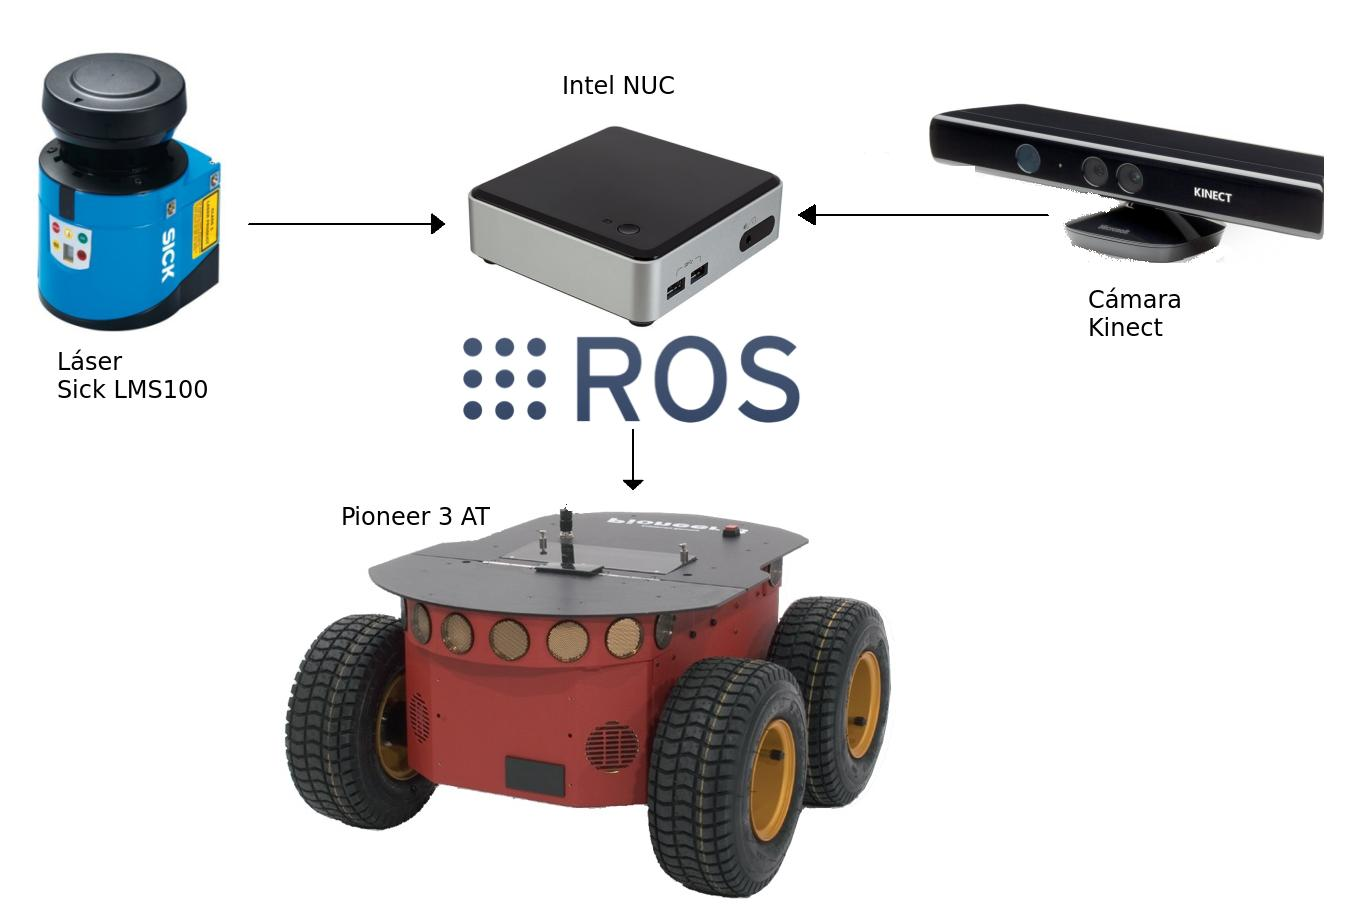
\includegraphics[width=0.8\textwidth]{figuras/esquema_robot.jpg}
\caption{Esquema del sistema rob�tico utilizado en el proyecto} \label{fig:esquema_robot1}
\end{figure}

Las consignas de navegaci�n se realizan mediante un ordenador externo cualquiera conectado a una red inal�mbrica o mediante consignas de voz, en las que se indica al robot las tareas de navegaci�n a realizar (avanzar, girar, seguir a una persona...) o un punto del entorno al que dirigirse.\\

Todas estas implementaciones est�n desarrolladas bajo el entorno ROS, lo cual permite a�adir funcionalidades de manera m�s r�pida y menos laboriosa, como es el caso del control mediante comandos de voz o la interacci�n mediante sonidos. Es el caso tambi�n del simulador de rob�tica Gazebo, que se integra como funcionalidad en ROS y que ha servido para testear el sistema y aportar las pruebas te�ricas pertinentes para luego aplicarlas en el robot real.\\

Para concluir, podemos decir que este proyecto se encarga de integrar ROS como sistema en un ordenador de abordo incorporado en el robot que permita conectarse con los sensores y realizar la construcci�n de mapas y navegaci�n aut�noma mediante el c�culo de mapas y trayectorias globales y locales, realizar los movimientos del robot, as� como reconocer consignas de voz o de teleoperaci�n.

\paragraph{Palabras clave:} palabraclave1, palabraclave2, palabraclave3.

\selectlanguage{USenglish}
\chapter{Abstract}

Achieving navigation and guidance of mobile robot comes up as a tool for rescue purposes in places where humans can't access or that involve a high risk for life. Many of those repetitive and fatigating tasks could be done with a robust and capable mobile robot.\\

An autonomous robot is, by the way, an essential part in rescue, inspection and exploration tasks developed in dangerous or non-reacheable places, such as the surface of other planets. Moreover, social tasks are taking more and more interest in our nowadays, such as assitance for humans in pubic places, interaction with the environment or a safer navigation in the cities. Autonomous car navigtion is a good example of this.\\

This final degree project is about guidance and control of a four-wheel mobile robot with a skid-steer configuration. It is equipped with a sort of sensors, allowing it to make positioning and orientation in the environment. There is also a main sensor capturing the enviaronment en three dimension and an additional one doing it in two dimensions.\\

Sensor data is used to build two dimensional maps of the exploration place as well as to take care of dynamical obstacles. The robot can build maps formed by cells where to incorpore or raytrace static and dynamic obstacles, calculate the proper trajectory plan and head for a destination point avoiding obstacles in its way.\\

All this information, data processing, trajectory calculation and movement execution is done in an onboard computer inside the robot. It uses the Robot Operating System software (known as ROS), which offers a commmon interface to communicate the robot with sensors and navigation algorithms.\\

The navigation process is divided in two parts. Firstly, a global obstacle map is done and static objects are addded, then the most suitable trajectory is planned. This is called global navigation. Secondly, a dynamic map is done and sensor data incorpores obstacles near the robot. Immediatly, a possible trajectory is planned following the original trajectory of the global navigation but avoiding the obstacles. This is called reactive or local navigation.\\

Finally, a movement algorithm does the control over the robot. It calculates movements to make the robot go forward, backward, turn around or make recovery tasks to recover if the robot has lost the trajectory path or it is stucked at any point.\\

Apart from autonomous navigation, the robot also has a telecontrol system from an outside computer and an algorithm to detect frontal objects in three dimensions (pointclouds) that can guide the robot. This is how it can navigate following a person when it is walking or another robot in front of it.\\

Pioneer 3 AT robot is the one used in this project (Figure \ref{fig:esquema_robot2}). It is the specific platform and all real tests have been made with it. This robots is equipped with a two dimension laser scanner (Sick LMS100 sensor) and a three dimensional sensor (Kinect sensor). The navigation computation is done in an onboard compact computer (Intel NUC *** computer).\\

\begin{figure}[htp]
\centering
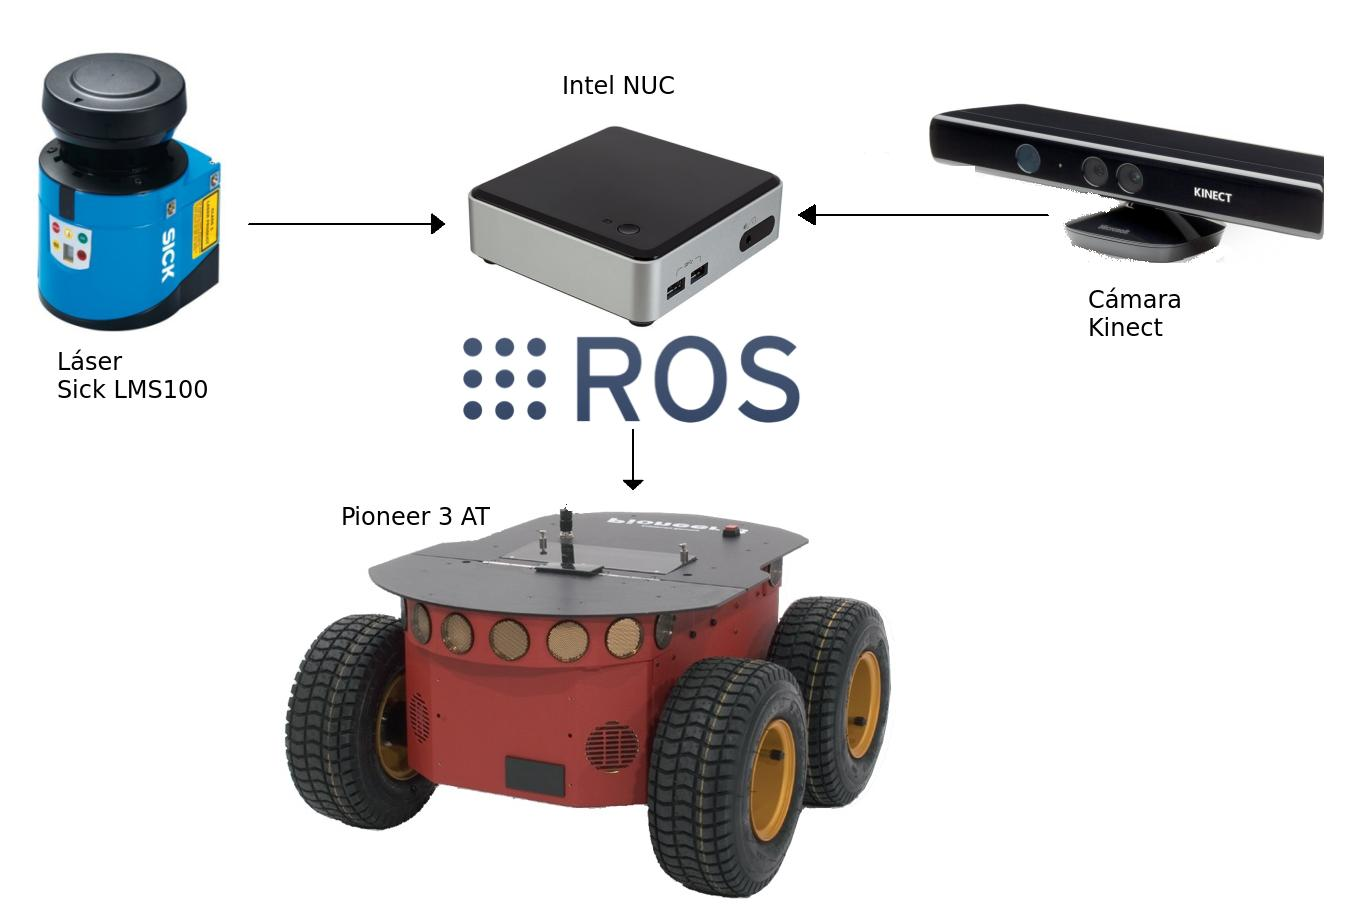
\includegraphics[width=0.8\textwidth]{figuras/esquema_robot.jpg}
\caption{Diagram of the robotic system used for this project} \label{fig:esquema_robot2}
\end{figure}

The navigation commands are sent from an outside computer connected to the same wireless network or from voice navigatin commands speaking directly to the robot (go forward, backward, turn right...) or a point in the map to move forward.\\

All those implementations are developed under ROS framework. This is why additional features can be added in a faster and effortless way. Tha is the case of the robot simlator Gazebo, which integrates as an add-on in ROS. Gazebo has been used to perform tests in navigation and to check theorical concepts to lately incorporate them in the real robotic system.\\

To conclude, it can be said that this project integrates ROS as a robotic system in an onboard computer and connects to sensors to perform tasks such as building maps or navigation from one point to other. The system calculates local and global maps and trajectories, makes movements according to them, as well as recognises voice or teleoperation commands.\\

\paragraph{Palabras clave:} PalabraClave1, keyword2, keyword3.

\selectlanguage{spanish}

%genera �ndice
\tableofcontents

%�ndice de figuras.
\listoffigures

%�ndice de tablas.
\listoftables

\listofcodes

%empieza la parte descriptiva del trabajo
\mainmatter

\chapter{Introducci�n}

Esta primera secci�n ser� un apartado previo para poner en contexto al lector sobre la rob�tica m�vil en general y a todo el desarrollo del proyecto ''Guiado de un robot m�vil basado en ROS y Kinect'' en particular.

En esta secci�n explicaremos qu� consiste y cu�les son los principales problemas de la rob�tica m�vil as� como las motivaciones para el desarrollo del proyecto.

\section{Rob�tica}

a historia de la rob�tica tiene su precursor en la mec�nica y los mecanismos desarrollados para imitar el movimiento y funciones de los seres vivos. Los antiguos egipcios ya empleaban mecanismos para mover los brazos de las estatuas y los griegos utilizaban sistemas hidr�ulicos para adornar sus templos.

Podemos decir que en torno al siglo XVII es cuando se inicia la historia de la rob�tica actual. En concreto, cuando Jacques de Vaucanson en 1745 invent� el primer telar autom�tico de la historia. Tambi�n construy� lo que se denomin� como aut�matas en la �poca, con obras como El flautista, El tamborilero o El pato, obra conocida como una de las pioneras en la historia de la rob�tica \cite{rojas2007historia}.

M�s tarde, Joseph Jacquard inventa en 1801 una m�quina textil programable mediante tarjetas perforadas refinando la tecnolog�a empleada por Vaucason \cite{martinez2000breve}. A�os m�s tarde, la Revoluci�n Industrial impuls� el desarrollo de m�quinas que automatizaban tareas que antes realizaban las personas dando paso a la hisotiria de la automatizaci�n industrial.

Antes ya se hab�an desarrollado algunos mecanismos autom�ticos como el Le�n mec�nico creado por Leonardo Da Vinci en el siglo XVI \cite{duliep2012leonardo}, que abr�a su pecho mostrando el escudo del rey Luis XII, o el Hombre de palo, un aut�mata de madera construido por Juanelo Turriano que andaba y mov�a la cabeza, ojos, boca y brazos.

La palabra ``robot'' comenz� a utilizarse en el mundo del teatro y de la ciencia ficci�n. Una obra checoslovaca publicada en 1917 por Karel Kapek, denominada Rossum's Universal Robots, dio lugar al t�rmino robot. La palabra checa ``Robota'' significa servidumbre o trabajador forzado, y cuando se tradujo al ingles se convirti� en el t�rmino robot. Como ejemplo de ciencia ficci�n se podr�a mencionar al escritor Isaac Asimov por la publicaci�n sobre las tres leyes de la rob�tica \cite{asimov1987robots}.

Los primeros robots llamados como tal fueron creados en 1958 y eran de tipo teleoperados, con el objetivo de manipular elementos sin riesgo para el operario. Este tipo de robots consisten en un sistema maestro-esclavo en el que los movimientos realizados por el maestro son transmitidos mec�nicamente a cierta distancia y reproducidos por el robot esclavo.

A�os m�s tarde, se comenz� a utilizar la tecnolog�a electr�nica y el uso del servocontrol, sustituyendo la transmisi�n mec�nica por otra el�ctrica. Ejemplos de estos manipuladores fue el realizado por Ralph Mosher, Handy-Man, consistente en dos brazos mec�nicos teleoperados mediante un maestro del tipo denominado exoesqueleto.

La sustituci�n del operador en este tipo de sistemas por un programa de ordenador que controlase los movimientos del manipulador dio paso al concepto de robot \cite{barrientos2007}.

\section{Rob�tica M�vil}

Pr�cticalmente cualquier robot consta de alguna parte m�vil que le permite realizar alg�n tipo de tarea, sin embargo nos referimos a la <<rob�tica m�vil>> como el �rea de la rob�tica que estudia los robots con capacidad para trasladarse en un ambiente dado.

Los robots m�viles son aquellos que tienen la capacidad de desplazarse utilizando alg�n sistema locomoci�n como pueden ser ruedas, patas, girar sobre s� mismos... Estos robots se diferencian respecto a los robots fijos que permanecen anclados a una superficie, como un brazo rob�tico industrial. Tampoco debe confundirse con los robots destinados a desplazarse por otros medios como agua o aire, ya que estar�amos entrando en el �rea de la rob�tica acu�tica/submarina o rob�tica a�rea respectivamente. Podemos decir por tanto que la rob�tica m�vil se refiere a robots que se mueven en el entorno terrestre.

Las aplicaciones dentro de la rob�tica m�vil pueden ser m�ltiples: exploraci�n de entornos peligrosos, exploraci�n espacial o minera, misiones e b�squeda y rescate de personas, telepresencia, automatizaci�n de procesos, transporte aut�nomo, vigilancia, inspecci�n y reconocimiento del terreno o utilizados como plataformas m�viles que incorporan otros sistemas rob�ticos como podr�an ser un brazo manipulador.

La rob�tica m�vil surgi� como manera extender el campo de la rob�tica hacia robots que anclados a un punto fijo. La capacidad de estos robots para desenvolverse en entornos diferentes ofrec�a la posibilidad de abrir nuevas lineas de investigaci�n y automatizar tareas que estaban asociadas con la navegaci�n y localizaci�n.

Los primeros pasos dentro de la rob�tica m�vil eran motivados por la idea de introducir la mayor autonom�a posible a los robots, tanto en terminos de suministro de energ�a como en computaci�n para realizar las tareas de planificaci�n, percepci�n y control.

Ampliar **REFERENCIAS A LIBROS**



\section{Motivaci�n del proyecto}
Dotar a un robot de la capacidad de navegar aut�nomamente puede ser una alternativa imprescindible en el caso de que se necesite explorar un entorno que no sea f�cilmente accesible para el ser humano o que conlleve cierto riesgo.

Cualquier proyecto que desarrolle la automatizaci�n de un proceso es ya una motivaci�n, puesto que se va a dise�ar una m�quina que sea capaz de realizar una tarea que antes solo pod�a realizarse por un ser humano. Adem�s, dichas tareas realizadas por un robot pueden realizase, en principio, con una mayor precisi�n y con mayor repetibilidad debido a que se elimina el factor del cansancio.

Este proyecto tambi�n viene motivado por la integraci�n de ROS dentro de una plataforma m�vil. Con esta plataforma de desarrollo software podemos explorar un concepto diferente de programaci�n en rob�tica, que ofrece caracter�sticas como:
\begin{itemize}
    \item Abstraerse de la programaci�n a bajo nivel.
    \item Reutilizar software ya desarrollado (nodos).
    \item Interfaz de comunicaci�n com�n.
    \item Escalabilidad del sistema.
    \item Simulaci�n mediante Gazebo.
    \item Visualizaci�n gr�fica de la informaci�n aportada por sensores.
    \item Transformaci�n entre los diferentes sistemas de coordenadas.
\end{itemize}

Utilizar sensor de bajo coste Kinect es otra de las motivaciones de este proyecto debido a que este sensor de bajo coste permite obtener informaci�n en tres dimensiones del entorno, pudi�ndose realizar una navegaci�n basada solamente en este sensor adem�s de reconocer objetos por su forma y realizar el guiado del robot detectando objetos.

De las aplicaciones que m�s han servido como motivaci�n para el desarrollo de este proyecto ha sido la automatizaci�n de las tareas de conducci�n de autom�viles \cite{cocheautonomo}, un sector que se encuentra en auge y que comienza a dar sus primeros pasos en el mundo real \cite{nevadagoogle}.

Tambi�n los robots de exploraci�n espacial de la NASA, en especial a su �ltimo rover en Marte, Curiosity \cite{marsNASA}, que permite explorar el entorno �rido de la superficie marciana con un alto grado de autonom�a en las labores de inspecci�n y an�lisis de elementos.

\section{Alcance y objetivos del proyecto}

En esta secci�n se define el alcance y los objetivos de este proyecto, es decir, lo que se pretende conseguir con este proyecto y hasta donde puede llegar.

\subsection{Prop�sito y alcance}

El prop�sito de este proyecto es el control autom�tico de un robot m�vil utilizando ROS. Lo que se pretende es implementar la navegaci�n aut�noma del robot bas�ndose en un control reactivo a partir de la informaci�n obtenida a trav�s del sensor Kinect.

El alcance del proyecto requiere m�ltiples elementos de trabajo:

En primer lugar, requiere un conocimiento previo del sistema hardware, como es el robot Pioneer 3 AT as� como el sensor Kinect. C�mo integrar estos elementos y acceder a la informaci�n que aportan sus sensores y comandar al robot para que realice movimientos.

En segundo lugar, requiere un conocimiento del entorno de desarrollo ROS. Las herramientas software de las que dispone, el funcionamiento interno y la manera de programar e interaccionar con los diferentes elementos, el aprendizaje y comprensi�n.

En tercer lugar, incorporar los sensores pertinentes para obtener la informaci�n que permita al robot posicionarse en el entorno.

En cuarto lugar, implementar los ajustes necesarios para que el robot pueda operar utilizando el entorno de navegaci�n ofrecido por ROS. Realizar una configuraci�n �ptima de los sensores y realizar las pruebas reales para el c�culo de trayectorias y el control reactivo del robot.

Por �ltimo, realizar la integraci�n del sistema dentro de la plataforma rob�tica. Disponer de todo lo necesario para que el robot quede totalmente adaptado al sistema ROS e integrado con el sensor Kinect y los sensores pertinentes.

\subsection{Objetivos}

El objetivo de este proyecto es realizar el control de un robot m�vil para que sea un robot aut�nomo, bas�ndose en la informaci�n que da la odometr�a y la nube de puntos que proporciona un sensor que captura el entorno en 3 dimensiones como el sensor Kinect. Este control debe realizarse con la ayuda del software ROS, integr�ndolo como parte del sistema rob�tico para que sirva de soporte al desarrollo del proyecto.

El robot debe ser capaz de localizarse y situarse en el entorno, el sensor Kinect ofrecer� informaci�n sobre los objetos alrededor del robot, y el software desarrollado para ROS deber� ser capaz de hacer un control reactivo sobre los movimientos para permitir al robot moverse por interiores y guiarlo hacia un punto indicado.

Los objetivos principales de este proyecto ser�n los siguientes:
\newcounter{enum2} % creamos un contador par la enumeraci�n. 
\begin{enumerate}[a)]
\item El primer objetivo es familiarizarse con el control de los robots m�viles y m�s concretamente en el control del robot Pioneer 3 AT. Familiarizarse con el sensor Kinect y con el software necesario para su uso. Y familiarizarse con el framework ROS y sus herramientas para el desarrollo de sistemas rob�ticos.
\setcounter{enum2}{\value{enumi}}
\end{enumerate}

\begin{enumerate}[a)]
\setcounter{enumi}{\value{enum2}}
\item Detecci�n de obst�culos simples con el sensor Kinect para su inclusi�n posterior en el sistema de navegaci�n del robot.
\setcounter{enum2}{\value{enumi}}
\end{enumerate}

\begin{enumerate}[a)]
\setcounter{enumi}{\value{enum2}}
\item Telecontrol del robot Pioneer 3 AT a partir del software ROS para realizar un controlador manual desde un ordenador externo.
\setcounter{enum2}{\value{enumi}}
\end{enumerate}

\begin{enumerate}[a)]
\setcounter{enumi}{\value{enum2}}
\item Realizar un sistema de navegaci�n aut�nomo que sea capaz de dirigir el robot bas�ndose en la informaci�n aportada por el sensor Kinect y otro tipo de sensores embebidos.
\setcounter{enum2}{\value{enumi}}
\end{enumerate}

De los objetivos anteriores podemos desgranar algunos objetivos intermedios:

\newcounter{enum3}
\begin{enumerate}[a)]
\item Comprender el funcionamiento de ROS y la integraci�n e interacci�n del software desarrollado bajo este entorno.
\setcounter{enum3}{\value{enumi}}
\end{enumerate}

\begin{enumerate}[a)]
\setcounter{enumi}{\value{enum3}}
\item Control del movimiento del robot Pioneer 3 AT a trav�s de ROS, as� como la obtenci�n de la informaci�n de la odometr�a, estado de la bater�a, encendido de motores...
\setcounter{enum3}{\value{enumi}}
\end{enumerate}

\begin{enumerate}[a)]
\setcounter{enumi}{\value{enum3}}
\item Puesta en marcha el sistema de navegaci�n para robots de ROS conocido como ''Navigation Stack'' y exploraci�n de las capacidades del sistema.
\setcounter{enum3}{\value{enumi}}
\end{enumerate}

\begin{enumerate}[a)]
\setcounter{enumi}{\value{enum3}}
\item Valorar el uso de sensores adicionales y buscar una disposici�n �ptima de los mismos para integrarlos en el sistema de navegaci�n y en la arquitectura hardware del propio robot.
\setcounter{enum3}{\value{enumi}}
\end{enumerate}

  
  %partes fin\label{ale}s del trabajo: conclusiones, bibliografia y anexos
  
\chapter{Estado del arte}

La rob�tica m�vil vive actualmente un momento de gran desarrollo para multitud de aplicaciones en entornos diversos, desde espacios abiertos con orograf�a accidentada y condiciones clim�ticas adversas **proyecto robot catastrofes** **proyecto DARPA big dog**, entornos controlados y espacios interiores conocidos como la automatizaci�n de tareas de almacenaje de productos **referencia robots amazon**, hasta orientaci�n y exploraci�n de espacios interiores desconocidos **robot creacion de mapas de edificios**.\\

De la misma forma, el inter�s en robots que sea capaces de reproducir las capacidades de un ser humano e incluso que pueda dar asistencia ya sea en entornos conocidos o no abre un �rea de posibilidades en las que los robots m�viles cobran importancia.\\

Los avances tanto el las caracter�sticas hardaware como software son notables aunque estas suelen variar dependiendo de la aplicaci�n a la que un robot est� destinado. En este cap�tulo trata de hacer un resumen del estadoactual de la rob�tica m�vil.\\


\section{Hardware en rob�tica m�vil}

Como hemos indicado previamente, la configuraci�n hardware de un robot m�vil var�a dependiendo de la aplicaci�n a la que vaya destinado. Es cierto que lo ideal para un robot ser�a disponer de una configuraci�n hardware com�n que fuera polivalente en los diferentes terrenos y situaciones, sin embargo, debido a la variedad de aplicaciones y dado que un robot suele destinarse a tareas espec�ficas, la elecci�n del hardware que mejor se adapta es una tendencia com�n en rob�tica.\\

Para seleccionar el hardaware debemos valorar el tipo de actuador que se requiere, entendi�ndose por actuador al dispositivo que genera el movimiento de los elementos que hacen que el robot m�vil se desplace. En rob�tica m�vil suelen utilizarse los actuadores de tipo ele�ctrico, ya que ofrecen unas prestaciones de potencia, controlabilidad y coste adecuados. Adem�s, ofrecen la posibilidad de que la alimentaci�n est� integrada en el robot, haci�ndolo independiente de una fuente de energ�a accesoria.\\

Los actuadores el�ctricos son, por tanto, los m�s utilizados. En concreto, los motores de corriente continua (Figura \ref{fig:motor_encoder}) ofrecen un f�cil control y f�cil acoplamiento a un encoder. Los encoder son sensores de posici�n que perminten conocer el giro de un eje de rotaci�n. Estos sensores son muy importantes en rob�tica m�vil, ya que a partir de la informaci�n que arrojan el robot tiene consciencia de su posici�n relativa, en el caso de los encoders incrementales, o su posici�n absoluta, en el caso de los encoders absolutos. **referencia a la secci�n de sesnsores**.\\

\begin{figure}[htp]
\centering
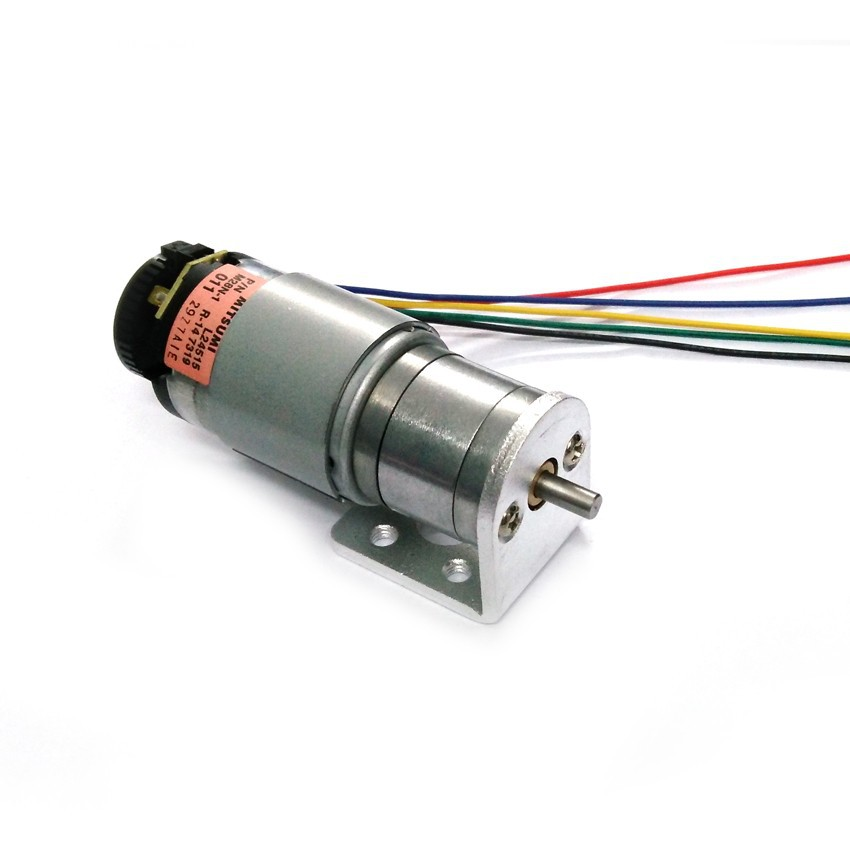
\includegraphics[width=0.4\textwidth]{figuras/motor_encoder.jpg}
\caption{Motor de corriente continua con encoder} \label{fig:motor_encoder}
\end{figure}

Existen otros tipos de actuadores el�ctricos que se utilizan en rob�tica, como puede ser el caso de los motores paso a paso, sin embargo su baja velocidad de giro no los hacen adecuados para robots m�viles.\\

La disposici�n de los actuadores determina la configuraci�n del robot. Centr�ndonos en robots que se desplazan mediante ruedas y descartando a los robots con patas, podemos distinguir las siguientes configuraciones: Ackerman, triciclo cl�sico, tracci�n diferencial, skid-steer, s�ncrona y omnidireccional.\\

**IMAGEN de las configuraciones LIBRO**

\newcounter{enum1} % creamos un contador par la enumeraci�n. 
\begin{enumerate}[a.]
  \item Configuraci�n Ackerman
\setcounter{enum1}{\value{enumi}} % le damos al contador el valor de la enumeraci�n.
\end{enumerate}

Consta de cuatro ruedas. Las ruedas motrices son las traseras o las delanteras, y �stas �ltimas se encargan adem�s de la direcci�n. Permite un desplazamiento a altas velocidades y la posibilidad de realizar giros con estabilidad. Esta configuraci�n es la que se utiliza en la industria del autom�vil.\\

\begin{enumerate}[a.]
\setcounter{enumi}{\value{enum1}} % reiniciamos enumeraci�n con el valor del contador.
  \item Triciclo cl�sico
\setcounter{enum1}{\value{enumi}}
\end{enumerate}

Consta de tres ruedas. Las ruedas motrices pueden ser las dos ruedas traseras o solo la delantera, que se encarga de la direcci�n. Este es el caso de los triciclos y de algunas bicicletas. Esta configuraci�n ofrece alto grado de maniobrabilidad penalizando la estabilidad del conjunto y realizar giros den 90�.\\

\begin{enumerate}[a.]
\setcounter{enumi}{\value{enum1}}
  \item Configuraci�n diferencial
\setcounter{enum1}{\value{enumi}}
\end{enumerate}

Consta de dos ruedas colocadas en el eje perpendicular a la direcci�n de desplazamiento del robot. Cada rueda es controlada por un motor, de tal forma que la diferencia de velocidad giro de una rueda respecto a otra determina el giro, avance o retroceso del robot. Los robots que presentan esta configuraci�n suelen utilizar una tercera rueda que gira libremente que sirver como apoyo (rueda loca). Es la configuraci�n t�pica de las sillas de ruedas y su caracter�stica principal es que permite realizar giros completos sobre s� mismo.\\

\begin{figure}[htp]
\centering
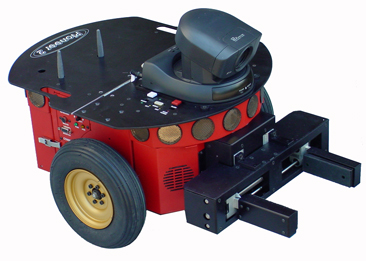
\includegraphics[width=0.3\textwidth]{figuras/pioneer3dx.jpg}
\caption{Robot de configuraci�n diferencial Pioneer 3 DX} \label{fig:pioneer_3dx}
\end{figure}

\begin{enumerate}[a.]
\setcounter{enumi}{\value{enum1}}
  \item Skid steer
\setcounter{enum1}{\value{enumi}}
\end{enumerate}

Consta de cuatro ruedas, todas ellas motrices, y su principio de funcionamiento es el mismo que el utilizado en la configuraci�n diferencial. Esta configuraci�n presenta las ventajas de la configuraci�n diferencial, pudiendo realizar giros sobre el eje del robot, pero presenta la desventaja de que las ruedas deben deslizarse lateralmente, por tanto existe un rozamiento que var�a en funci�n de la inclinaci�n el tipo de terreno que dificulta realizar un modelo cinem�tico.\\

Proporciona mucha tracci�n y estabilidad y suele encontrarse en aplicaciones relacionadas con la exploraci�n, veh�culos obra o veh�culos todo terreno (Figura \ref{fig:ejemplos_skid-steer}).\\

\begin{figure}[htp]
\centering
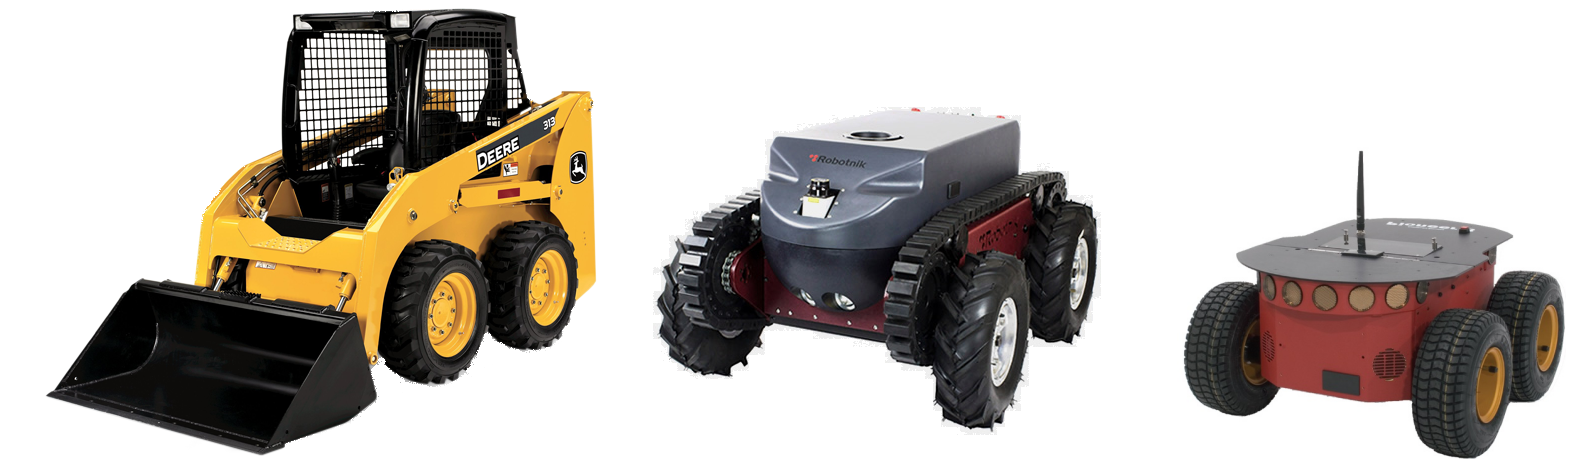
\includegraphics[width=0.7\textwidth]{figuras/skid-steer_examples.png}
\caption{Ejemplos de configuraci�n diferencial: Cargador frontal, Robotnik Guardian, Pioneer 3 AT} \label{fig:ejemplos_skid-steer}
\end{figure}

Este sistema es el que se utiliza tambi�n en los tanques de guerra, aunque en vez de neum�ticos se utilizan orugas, denominado configuraci�n por deslizamiento de cintas **Referencia**.\\

\begin{enumerate}[a.]
\setcounter{enumi}{\value{enum1}}
  \item Configuraci�n s�ncrona
\setcounter{enum1}{\value{enumi}}
\end{enumerate}

Conformado por tres o m�s ruedas acopladas mec�nicamente y dotadas de tracci�n, este sistema permite que todas las ruedas roten en la misma direcci�n y giren a la misma velocidad (Figura \ref{fig:configuracion_sincrona}). Es utilizada ampliamente en rob�tica para robots m�viles de interior, aunque est� siendo desplazada por la configuraci�n omnidireccional. \\

\begin{figure}[htp]
\centering
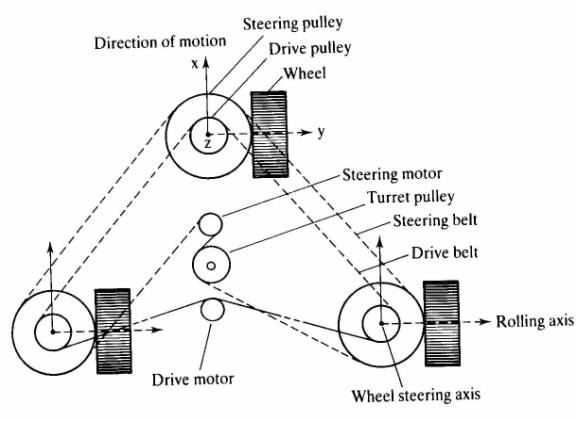
\includegraphics[width=0.4\textwidth]{figuras/configuracion_sincrona.png}
\caption{Configuraci�n s�ncrona} \label{fig:configuracion_sincrona}
\end{figure}

\begin{enumerate}[a.]
\setcounter{enumi}{\value{enum1}}
  \item Configuraci�n omnidireccional
\setcounter{enum1}{\value{enumi}}
\end{enumerate}

Consta de 3 ruedas cada una con un motor independiente, que permiten el desplazamiento en cualquier direci�n (Figura \ref{fig:configuracion_omnidireccional}). Las ruedas omnidireccionaes constan de una serie de rodillos con el eje de rotaci�n perpendicular a la direccio�n de avance.\\

\begin{figure}[htp]
\centering
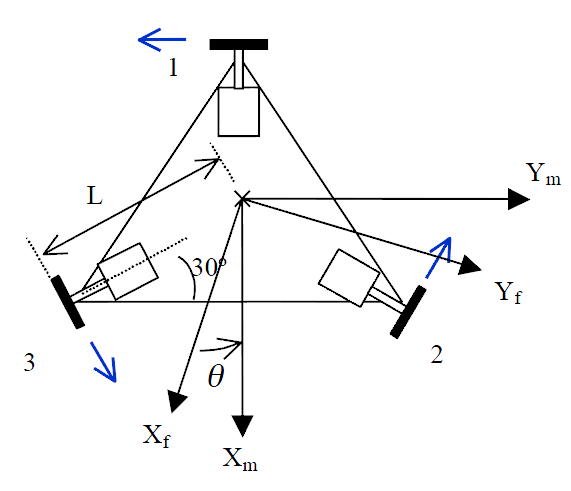
\includegraphics[width=0.4\textwidth]{figuras/configuracion_omnidireccional.png}\hspace{2cm}
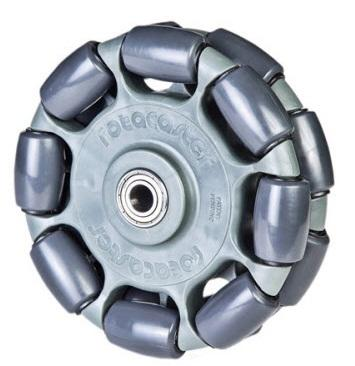
\includegraphics[width=0.3\textwidth]{figuras/rueda_omnidireccional.png}
\caption{Configuraci�n s�ncrona y rueda omnidireccional} \label{fig:configuracion_omnidireccional}
\end{figure}

Esta configuraci�n diferencial empieza a utilizarse en sistemas de 4 ruedas con las demonminadas ''Mecanum Wheels'' **REFERENCIAAA**, que son ruedas similares a las omnidireccionales pero con los rodillos colocados en cierto �ngulo (Figura \ref{fig:ruedas_mecanum}). La combinaci�n de los giros de cada una permiten al robot moverse en cualquier direcci�n.\\

\begin{figure}[htp]
\centering
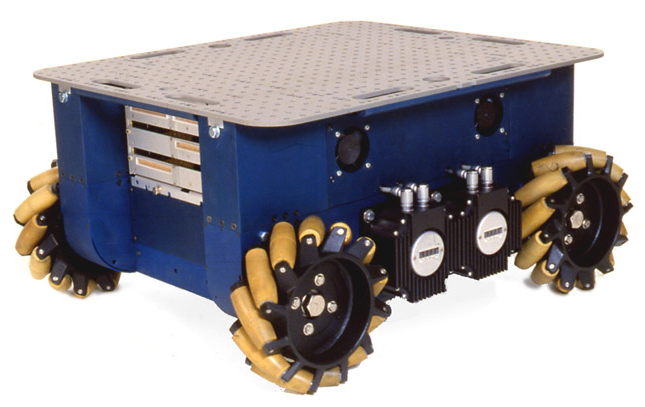
\includegraphics[width=0.4\textwidth]{figuras/mecanum-wheels_uranus.png}
\caption{Robot Uranus con ruedas tipo Mecanum} \label{fig:ruedas_mecanum}
\end{figure}

\section{Sensores en rob�tica m�vil}

Para que un robot pueda realizar tareas con una determinada precisi�n y velocidad debe conocer el entorno del sistema en el que se quiera actuar as� como el estado del robot en ese sistema.\\

Existen dos tipos de sensores, los sensores internos, que aportan informaci�n sobre la posici�n orientaci�n del robot, y los externos, que aportan informaci�n del entorno alrededor del robot.

\subsection{Sensores internos}

Dentro de los sensores internos, los sensores de posci�n primordiales son los encoders, tanto los de tipo incremental como los de tipo absoluto (Figura \ref{fig:esquema_encoder}). Su funcionamiento se basa en un foto-emisor y un foto-receptor que detectanel paso o no de luz a trav�s de un disco con ciertas marcas acoplado al eje de giro del actuador.

\begin{figure}[htp]
\centering
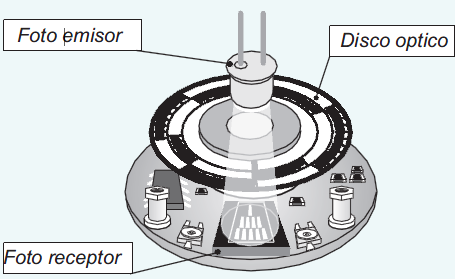
\includegraphics[width=0.4\textwidth]{figuras/encoder_absoluto.png}
\caption{Esquema de un encoder absoluto} \label{fig:esquema_encoder}
\end{figure}

Los sensores de velocidad son similares a los encoders pero miden la velocidad de giro del eje del actuador. La tacogeneratriz proporciona una tensi�n proporcional a la velocidd de giro.\\

Los sensores aceler�metros o inclin�metros, permiten conocer la inclinaci�n del robot en cada uno de sus ejes, as� como las aceleraciones producidas por su propio desplazamiento.\\

Existen otros sensores m�s sofisticados como las Unidades de medida inercial (IMU) (Figura \ref{fig:sensor_imu}). Son disposiivos que combinan las medidas de un gir�scopo y varios aceler�metros para determinar la posici�n relativa (x, y, z) y la orientaci�n (roll, pitch, yaw), velocidad y aceleraci�n respecto a un sistema de referencia.\\

\begin{figure}[htp]
\centering
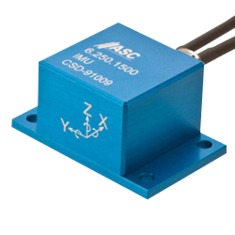
\includegraphics[width=0.4\textwidth]{figuras/sensor_imu.png}
\caption{Unidad de medida inercial, IMU} \label{fig:sensor_imu}
\end{figure}

Debido  a  que  la  aceleraci�n  se  ha  de  integrar  dos  veces  para  obtener  la 
posici�n,  el  error  crece  de  forma  cuadr�tica.  Luego  para  largos  periodos  de operaci�n las unidades IMU se deben de resetear con otros sensores tipo GPS.\\

\subsection{Sensores externos}

Los sensores externos son aquellos que nos aportan informaci�n sobre el estado del robot respecto al entorno o que nos da informaci�n sobre lo que ocurre alrededor de este.\\

Los sensores de presencia, como son los sensores de tipo inductivo, capacitivo, �ptico o mec�nico. Sea cual sea la naturaleza del sensor, su funci�n es la de detectar presencia. Un ejemplo de aplicaci�n a un robot m�vil ser�a una serie de sensores de presencia mec�nicos, denominados "fin de carrera", colocados en la parte delantera, de modo que al tocar alg�n obst�culo se tuviera conciencia de la presencia de un obst�culo.\\

Sensores de posicionamiento global GPS (Global Positioning System) que permiten determinar la posici�n de un objeto en todo el mundo, normalmente con una precisi�n de metros. El GPS funciona con una red de sat�lites con trayectorias sincronizadas que cobren toda la superficie de la tierra. El GPS lanza se�ales a los sat�lites y calculando el tiempoq ue tarda �stos en responder, se obtiene la posici�n por trianguaci�n.\\

Los sensores GPS se utilizan en robots m�viles que operan en el exterior y suen combinarse con otros sensores que ofrezcan una mayor precisi�n.\\

Los sensores de distancia son aquellos que nos dan una referencia de la longitud que existe a los objetos cercanos. Es el caso de los sensores e ultrasonidos, donde un emisor emite una onda ultras�nica y cuando es reflejada por un objeto se puede determinar la distancia a la que se encuentra midiendo el tiempo que tarda el sonido en ir y volver. Los sensores de distancia tambi�n pueden ser infrarrojos, funcionando de la misma manera.\\

Existen sensores de distancia que utilizan tecnolog�a l�ser para determinar la longitud de un punto a otro, se denominan Scanners l�ser. Estos sensores emiten rayos l�ser en un plano de 2 dimensiones y en un rango determinado, y midiendo el tiempo de vuelo del haz l�ser son capaces de obtener una medida muy precisa de la distancia.\\

Existen otro tipo de sensores de distancia que permiten obtener distancias a puntos de manera tridimensional. Algunos utilizan un sistema de doble c�mara conocidos como c�mara estereosc�pica (Figura \ref{fig:camara_estereoscopica}). Estos sesnores son capaces de obtener im�genes 3D con la informaci�n de dos im�genes tomadas a cierta distancia una de otra. Es el sensor m�s parecido a la visi�n humana.\\

\begin{figure}[htp]
\centering
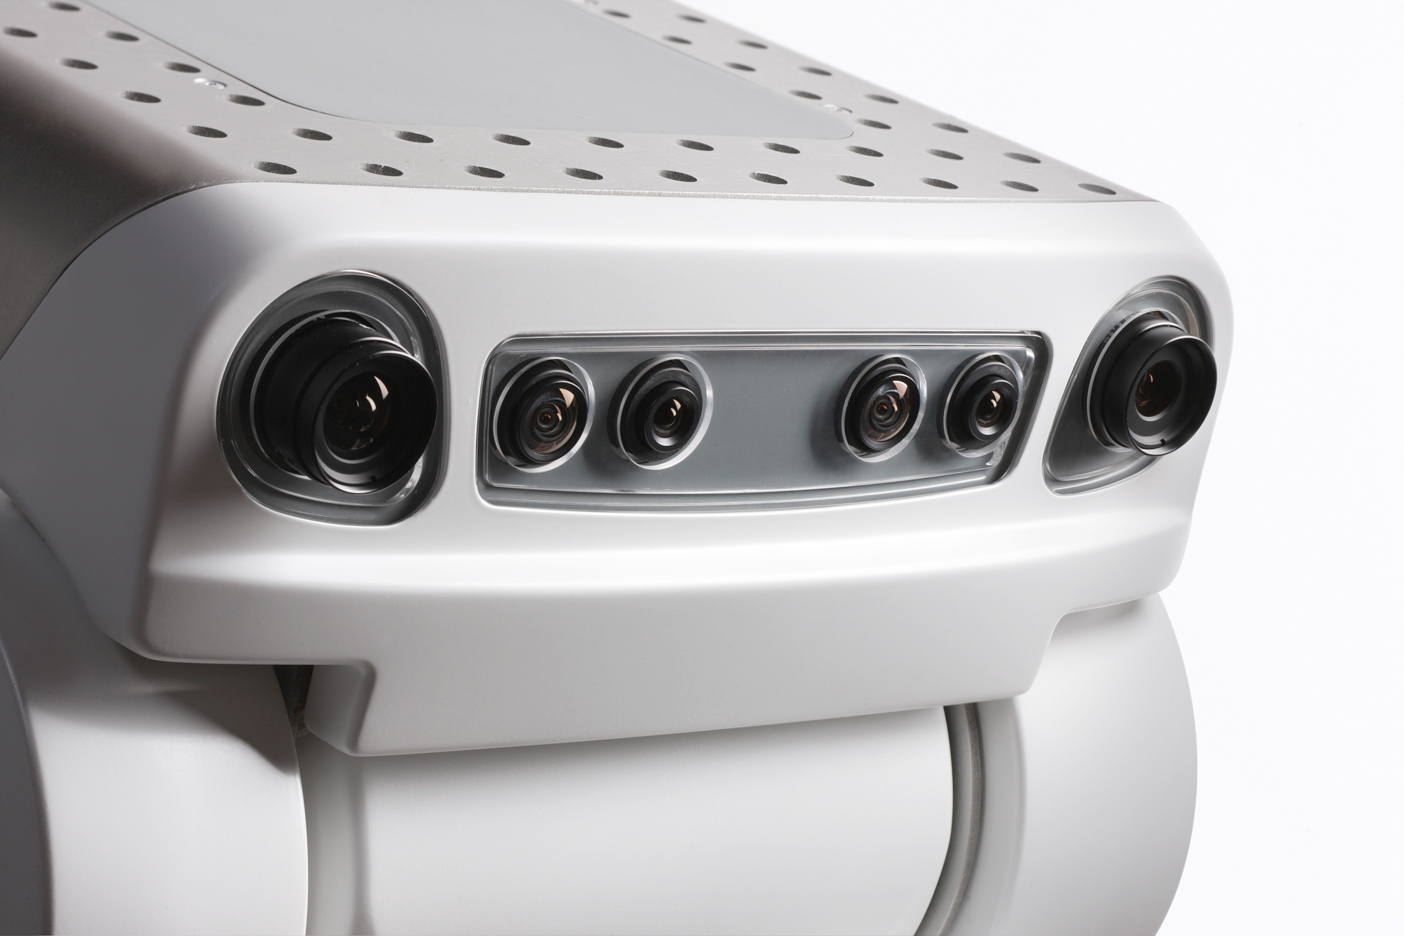
\includegraphics[width=0.4\textwidth]{figuras/pr2_stereocam.jpg}
\caption{C�mara estereosc�pica del robot PR2} \label{fig:camara_estereoscopica}
\end{figure}

Otros sensores de distancia en 3 dimensiones, son los sensores de tipo Infrarrojo **BUSCAR NOMBRE CORRECTO SENSORES 3D BOSCH**, como es el sensor Kinect, que ha se ha vuelto muy popular debido a su bajo coste y su buena respuesta.\\

Kinect es un dispositivo derrollado por PrimeSense**refenrecia** y distribuido por Microsoft para la vieoconsola Xbox 360 (Figura \ref{fig:sensor_kinect}).\\

Inicialmente permit�a controlar e interactuar con la consola XBOX sin necesidad de tener contacto f�sico con un controlador. Este sensor permite reconocer gestos, comandos de voz, objetos e im�genes; esto hace que tenga mucho inter�s en el mundo de la rob�tica.

\begin{figure}[htp]
\centering
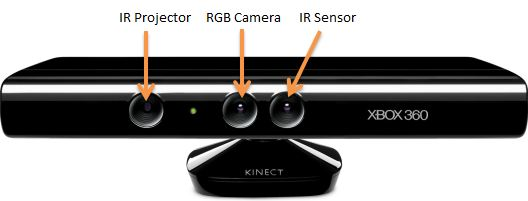
\includegraphics[width=0.4\textwidth]{figuras/kinect.jpg}
\caption{Sensor de 3 dimensiones Kinect para Xbox 360} \label{fig:sensor_kinect}
\end{figure}

Para captar el entorno en 3 dimensiones, Kinect incluye una c�mara de v�deo RGB, un emisor de haz infrarrojo y una c�mara infrarroja.

\section{Control en la rob�tica m�vil actual}

El control del movimento en los robots m�viles con ruedas puede describirse, de manera general, en cuatro tareas fundamentales: localizaci�n y orientaci�n, planificaci�n de trayectoria, seguimiento de la misma y evasi�n de los obst�culos.\\

\subsection{Localizaci�n y orientaci�n en un entorno}
Normalmente, uno de los mayores problemas que conciernen a la navegaci�n de robots m�viles consiste en la determinaci�n de su localizaci�n respecto a un mapa en funci�n de la informaci�n captada por los sensores.. No basta con situar una referencia global, si no que es imprescindible conocer la posici�n relativa respecto a los posibles obst�culos, tanto m�viles como est�ticos, de su entorno. Para esta tarea existen diferentes opciiones, como utilizar mapas introducidos en el robot, o bien elaborar un mapa de manera simult�nea al movimiento del robot por un lugar, como si se tratase de un robot de exploraci�n. Es lo que se conocde como SLAM (Simultaneous Localization and Mapping)**refenrecia**.

Uno de las motivaciones para el uso de esta t�cnica es la construcci�n de mapas desde el punto de vista del robot, as� como el ruido que se genera en los sensores de posici�n internos del robot que miden la odometr�a. Sin embargo, esta t�cnica en ocasiones puede producir efectos no deseados, como incorrecciones en el mapa debido a su alto coste computacional o variaciones debidas a objetos que se mueven en torno al robot.

\section{Aplicaciones actuales de la rob�tica m�vil}

vhbjklm�vhjbknlm�knjbhvgcvbjnklm�kjnb.\\

\chapter{Alcance y objetivos del proyecto}

En este cap�tulo se define el alcance y los objetivos de este proyecto, es decir, lo que se pretende conseguir con este proyecto y hasta donde puede llegar.\\

\section{Prop�sito y alcance}

El prop�sito de este proyecto es el control autom�tico de un robot m�vil utilizando ROS. Lo que se pretende es implementar la navegaci�n aut�noma del robot bas�ndose en un control reactivo a partir de la informaci�n obtenida a trav�s del sensor Kinect.\\

El alcance del proyecto requiere m�ltiples elementos de trabajo:\\

En primer lugar, requiere un conocimiento previo del sistema hardware, como es el robot Pioneer 3 AT as� como la sensor Kinect. C�mo integrar estos elementos y acceder a la informaci�n que aportan sus sensores y comandar al robot para que realice movimientos.\\

En segundo lugar, requiere un conocimiento del entorno de desarrollo ROS. Las herramientas software de las que dispone, el funcionamiento interno y la manera de programar e interaccionar con los diferentes elementos, el aprendizaje y comprensi�n.\\

En tercer lugar, incorporar los sensores pertienentes para obtener la informaci�n que permita al robot posicionarse en el entorno.\\

En cuarto lugar, implementar los ajustes necesarios para que el robot pueda operar utilizando el entorno de navegaci�n ofrecido por ROS. Realizar una configuraci�n �ptima de los sensores y realizar las pruebas reales para el c�culo de trayectorias y el control reactivo del robot.\\

Por �ltimo, realizar la integraci�n del sistema dentro de la plataforma rob�tica. Disponer de todo lo necesario para que el robot quede totalmente adaptado al sistema ROS e integrado con el sensor Kinect y los sensores pertinentes.

\section{Objetivos}

El objetivo de este proyecto es realizar el control de un robot m�vil para que sea un robot aut�nomo, bas�ndose en la informaci�n que da la odometr�a y la nube de puntos que proporciona un sensor que captura el entorno en 3 dimensiones como el sensor Kinect. Este control debe realizarse con la ayuda del software ROS, integrandolo como parte del sistema rob�tico para que sirva de soporte al desarrollo del proyecto.\\

El robot debe ser capaz de localiarse y situarse en el entorno, el sensor kinect ofrecer� informaci�n sobre los objetos alrededor del robot, y el software desarrollado para ROS deber� ser capaz de hacer un control reactivo sobre los movimientos para permitir al robot moverse por interiores y guiarlo hacia un punto indicado.\\

Los objetivos principales de este proyecto ser�n los siguientes:\\

\newcounter{enum1} % creamos un contador par la enumeraci�n. 
\begin{enumerate}[a.]
  \item Configuraci�n Ackerman
\setcounter{enum1}{\value{enumi}} % le damos al contador el valor de la enumeraci�n.
\end{enumerate}

texto.\\

\begin{enumerate}[a.]
\setcounter{enumi}{\value{enum1}} % reiniciamos enumeraci�n con el valor del contador.
  \item Triciclo cl�sico
\setcounter{enum1}{\value{enumi}}
\end{enumerate}

texto.\\

\begin{enumerate}[a.]
\setcounter{enumi}{\value{enum1}}
  \item Configuraci�n diferencial
\setcounter{enum1}{\value{enumi}}
\end{enumerate}


\chapter{Desarrollo del proyecto}

\section{Planteamiento}

\section{Planificaci�n del proyecto}

\section{Tecnolog�as empleadas en el proyecto}

\section{Herramientas utilizadas en el proyecto}

\section{Hardware}
En esta parte se explica detalladamente el hardware empleado en el desarrollo del proyecto.

\subsection{Pioneer 3 AT}

El robot Pioneer 3 AT (Figura \ref{fig:pioneer3at}), perteneciente a la empresa Adept MobileRobots, es un robot de cuatro ruedas en configuraci�n skid-steer y todo terreno (AT, All Terrain) de operaci�n e investigaci�n en laboratorio.\\

\begin{figure}[htp]
\centering
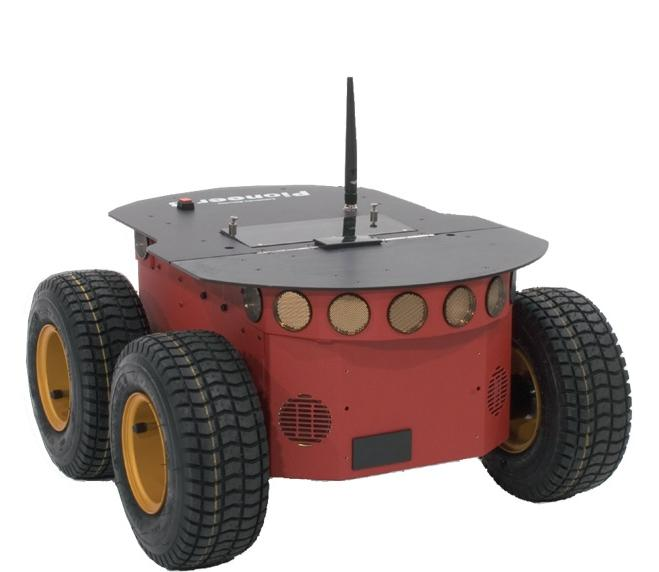
\includegraphics[width=0.4\textwidth]{figuras/pioneer_3_at.jpg}
\caption{Robot Pioneer 3-AT} \label{fig:pioneer3at}
\end{figure}

Su configuraci�n en skid-steer permite un control relativamente simple utilizando el modo diferencial para poder realizar giros con gran maniobrabilidad, sin embargo, esta configuraci�n depende mucho del tipo de suelo, con lo que se pierde precisi�n.\\

Este robot dispone de bater�as, interruptor con parada de emergencia, dos motores de corriente continua para cada par de ruedas con transmisi�n mediante correa, encoders para leer la odometr�a y un microcontrolador con firmware ARCOS.\\

Ademas cuenta con un peque�o computador interno conectado al microcontrolador que puede utilizarse para realizar operaciones de manera aut�noma.\\

El cuerpo del robot es de aluminio y su parte delantera as� como superior es f�cilmente desmontable para realizar las conexiones pertinentes y acceder al ordenador de a bordo y la placa microcontroladora. En la plataforma superior se sit�a el panel de control (Figura \ref{fig:panel_control})para acceder al ordenador de abordo conectando un monitor, teclado y rat�n, puerto serial RS-232, botones de encendido y reset varios leds indicadores de estado y de env�o y recepci�n de datos.\\

\begin{figure}[htp]
\centering
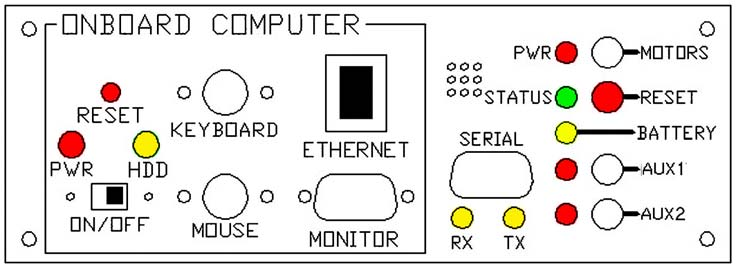
\includegraphics[width=0.6\textwidth]{figuras/panel_control.png}
\caption{Panel de control del robot Pioneer 3-AT} \label{fig:panel_control}
\end{figure}

En la siguiente tabla (Tabla \ref{tabla_pioneer3at}) se describen las principales caracter�sticas del robot.\\

% Please add the following required packages to your document preamble:
% \usepackage{graphicx}
\begin{table}[!h]
\centering
\resizebox{\textwidth}{!}{%
\begin{tabular}{c c}
\hline
{\bf Especificaciones} & {\bf Pioneer 3 AT} \\ \hline
Largo & 508 mm \\
Ancho & 497 mm \\
Alto & 277 mm \\
Distancia al suelo & 80 mm \\
Peso & 12 kg \\
Carga �til & 32 kg \\
Cuerpo & Aluminio de 1.6 mm \\
Bater�as & 3 de 12 V ~Ah, estancas, plomo-�cido \\
Autonom�a & 4-8 horas \\
Sistema motriz & 4 ruedas motrices \\
Ruedas & Neum�ticos de Nylon \\
Di�metro de rueda & 222 mm \\
Ancho de rueda & 88 mm \\
Sistema de giro & Diferencial \\
radio m�xima curvatura & 40 cm \\
Radio de giro & 0 cm \\
M�xima velocidad de avance & 1.2 m/s \\
M�ximo escal�n & 10 cm \\
M�ximo hueco & 15.2 cm \\
Terreno & Asfalto, Tierra, C�sped, etc. \\
Encoders & 500 pulsos \\
Procesador & Hitachi H8S \\ \hline
\end{tabular}
}
\caption{Especificaciones del robot Pioneer 3 AT}
\label{tabla_pioneer3at}
\end{table}


\subsection{Sensor Kinect}

Kinect es un conjunto de sensores de bajo coste que lo convierte en una
herramienta excepcional (Figura \ref{fig:sensor_kinect}). Este dispositivo incluye una c�mara de v�deo RGB, una c�mara infrarroja de profundidad, un array de micr�fonos y altavoces, un aceler�metro y un peque�o motor que le permite hacer movimientos de inclinaci�n.\\

\begin{figure}[htp]
\centering
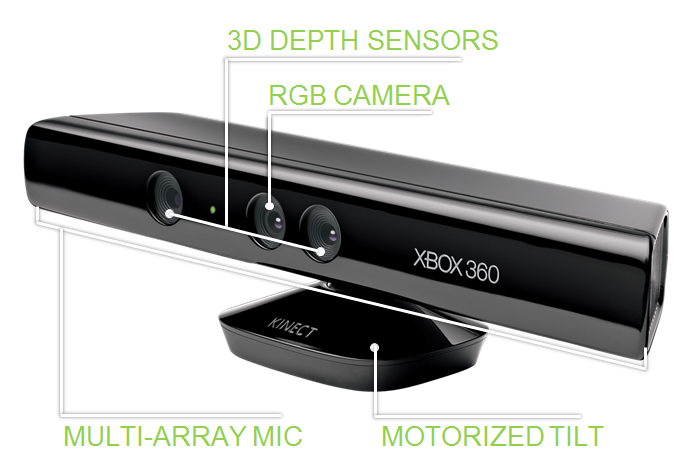
\includegraphics[width=0.6\textwidth]{figuras/sensor_kinect.png}
\caption{Sensor Kinect}
\label{fig:sensor_kinect}
\end{figure}

Su funci�n principal es la de percibir el entorno captando una serie de puntos que se ubican en las tres dimensiones. Su funcionamiento a grandes rasgos se basa en un emisor de infrarrojos a 830 nm que interact�ua con los objetos y una c�mara infrarroja que etecta la diferencia entre la proyecci�n anterior y la actual, obteniendo la distancia a cada objeto.\\

En primer lugar, el laser infrarrojo es emitido por Kinect con un patr�n
determinado, el cual no es sim�trico sino que tiene puntos aleatorios que se dispersa gracias a unas lentes de proyecci�n. Estos puntos aleatorios se reflejan en los objetos, los cuales ser�a posible verlos con una c�mara externa.\\

A continuaci�n, al sensor de Kinect MT9M001C12STM, que no es m�s que el
sensor CMOS de una c�mara en la que se le trata para que observe solo el
infrarrojo, obteniendo los puntos infrarrojos en el plano 2D. El motivo por el que podemos medir la profundidad de los objetos (su distancia) es porque sabemos el patr�n de c�mo emite el laser emisor, por tanto sabremos que si un punto no est� en el sitio que corresponde, se ha trasladado respecto al punto inicial y se le aplica la correspondiente transformaci�n, obteniendo finalmente los puntos de toda la nube en coordenadas cartesianas XYZ.\\

\begin{figure}[htp]
\centering
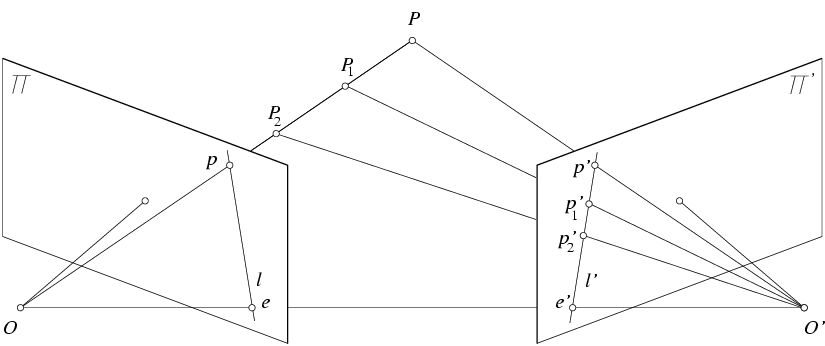
\includegraphics[width=0.8\textwidth]{figuras/proyecciones_kinect.png}
\caption{Proyecci�n de infrarrojos y obtenci�n de la nube de puntos}
\label{fig:sensor_kinect}
\end{figure}

La siguiente tabla muestra las especificaciones del sensor Kinect.

\begin{table}[!h]
\centering
\resizebox{\textwidth}{!}{
\begin{tabular}{c c}
\hline
{\bf Especificaciones} & {\bf Sensor Kinect} \\ \hline
Dimensiones del conjunto & 270mm x 50mm x 70mm \\
Fuente infrarroja & 830nm \\
Potencia & 60 mW \\
C�mara Infrarroja & MT9M001C12STM \\
Resoluci�n & 1200x960 pixeles \\
Frecuencia & 30 Hz \\
Tama�o pixel & 5.2um x 5.2um  \\
Pixeles activos & 1280H x 1024V \\
Campo de visi�n & 58o H, 45o V, 70o D \\
Interfaz de datos & Ethernet \\
Tensi�n de operaci�n & 10.8V - 20V DC \\
Consumo & 20 W \\
Peso & 1.1 Kg \\
Dimensiones & 105mm x 102mm x 152mm\\ \hline
\end{tabular}
}
\caption{Caracter�sticas del sensor l�ser Sick LMS100}
\label{tabla_sicklms100}
\end{table}

\subsection{L�ser SICK LMS100}

Aunque el planteamiento incial del proyecto planteaba la navegaci�n basada �nicamente en el sensor kinect, debemos mencionar el uso del sensor l�ser Sick LMS100 (Figura \ref{fig:sensor_sicklms100}).\\

\begin{figure}[htp]
\centering
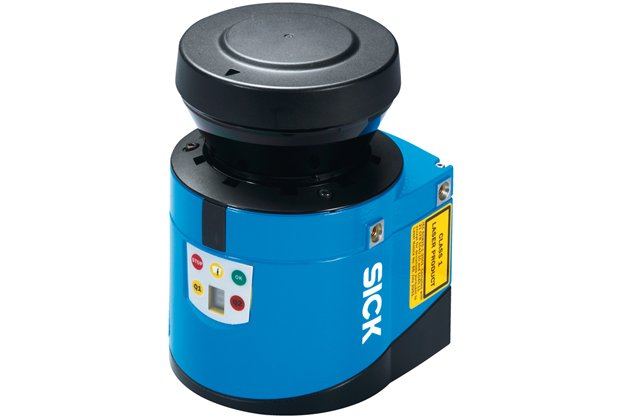
\includegraphics[width=0.6\textwidth]{figuras/SICK_LMS100.jpg}
\caption{Sensor escaner l�ser Sick LMS100}
\label{fig:sensor_sicklms100}
\end{figure}

Este es un sensor l�ser por infrarrojos de clase I (Inofensivo para el ojo humano), que obtiene la medida de distancias con gran preci�n y rapidez en un solo plano y realizando un barrido de 270� (Figura \ref{fig:sicklms100_rango}).\\

\begin{figure}[htp]
\centering
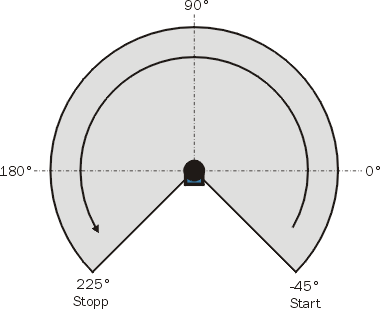
\includegraphics[width=0.6\textwidth]{figuras/sicklms100_rango.png}
\caption{Campo de visi�n del sensor l�ser Sick LMS100} \label{fig:sicklms100_rango}
\end{figure}

Este sensor est� colocado en la parte trasera del robot, enfocando hacia atr�s para cubrir un mayor rango y conocer todo el entorno alrededor del robot.\\

En la siguiente tabla (Tabla \ref{tabla_sicklms100}) se recogen sus caracter�sticas principales.\\

\begin{table}[!h]
\centering
\resizebox{\textwidth}{!}{
\begin{tabular}{c c}
\hline
{\bf Especificaciones} & {\bf Sick LMS100} \\ \hline
Campo de aplicaci�n & Interno \\
Fuente infrarroja & 905 nm \\
Clase L�ser & 1 (IEC 60825-1) \\
Campo de visi�n & 270� \\
Frecuencia de escaneo & 25Hz/50Hz \\
Resoluci�n angular & 0.25�/0.5� \\
Distancia de operaci�n & 0.05 - 20 m  \\
Tiempo de respuesta & 20 ms \\
Error & 30 mm \\
Interfaz de datos & Ethernet \\
Tensi�n de operaci�n & 10.8V - 20V DC \\
Consumo & 20 W \\
Peso & 1.1 Kg \\
Dimensiones & 105mm x 102mm x 152mm\\ \hline
\end{tabular}
}
\caption{Caracter�sticas del sensor l�ser Sick LMS100}
\label{tabla_sicklms100}
\end{table}

\chapter{Arquitectura}
Esta secci�n tiene como objetivo plantear la arquitectura general utilizada en el robot, las comunicaciones con el resto del hardware y con los nodos que proporcionan la informaci�n necesaria para que el robot sea totalmente aut�nomo.

\section{Arquitectura general}

A nivel de hardware utilizado en el proyecto, como es el propio robot, los sensores el ordenador de abordo el sistema se estructura de a siguiente manera:

\begin{enumerate}[i)]
\item  Robot Pioneer 3 AT: Este es el robot mencionado anteriormente, el cual debe ser configurado para acceder al puerto serie RS-232 de su placa controladora. Esto nos permite conectarnos con el firmware ARCOS **referencia** y comunicarnos a trav�s de la librer�a ARIA. De esta forma controlamos los motroes y podemos leer el valor de los encoders de la odometr�a.

\item Sensores: Tanto el sensor Kinect como el sensor l�ser ir�n alimentados a trav�s de las bater�as del robot y se comunicar�n con el ordenador de abordo a trav�s de puerto USB y ethernet respectivamente.

\item Ordenador Intel NUC: Ser� el ordenador de abordo encargado de ejecutar ROS y realizar todo el procesamiento necesario. Ir� equipado con el sistema operativo Ubuntu 14.04 por ser la �ltima versi�n estable disponible a fecha de la entrega del proyecto. Ir� conectado al robot mediante un convertidor RS-232 a USB, el sensor l�ser se comunica v�a ethernet y el sensor Kinect a trav�s de puerto USB igualmente. Tambi�n se conectar� el audio al altavoz integrado del robot.

\item Ordenador externo: Como se ha mencionado anteriormente, un ordenador externo opcional equipado con ROS podr� utilizarse para realizar tareas de a supervisi�n inal�mrica a trav�s de RViz y para realizar la teleoperaci�n del robot v�a TCP/IP integrado en ROS.
\end{enumerate}

\section{Arquitectura del proyecto}

El proyecto est� estructurado siguiendo la filosof�a de "paquetes" desarrollados en ROS. En el directorio ra�z del proyecto por tanto, encontraremos los paquetes necesarios para que el sistema funcione as� como los paquetes propios desarrollados:




\chapter{Entorno ROS}

La versi�n del software ROS utilizada para el desarrollo del proyecto ha tratado de ser siempre la m�s actual posible, ya que eso nos asegura mantener la compatibilidad en futuros trabajos y que el software est� actualizado.

La versi�n utilizada fue ROS Indigo Igloo desde el comienzo del proyecto, bajo el sistema operativo Ubuntu 14.04. A fecha de entrega del proyecto existe una versi�n m�s actualizada del software ROS, sin embargo se desestim� su uso debido a que a�n no era una versi�n estable y algunos paquetes no se encontraban disponibles para tal versi�n.

Dentro de ROS exixten diferentes conceptos como los nodos, los rostopics, rosservices...

- Nodos.
- Servicios.
- Rostopics.

\subsection{Funcionamiento de ROS}

\section{Configuraci�n de ROS}
Para la instalaci�n de ROS es necesario seguir ciertos pasos bien explicados en la wiki de su p�gina.

Para el ordenador de abordo del robot utilizamos la versi�n completa del software.

A�adimos nuestra variable de entorno para buscar en los directorios de ros cuando ejecutemos los nodos.

Para el desarrollo dentro de ROS se utiliza el entorno de desarrollo Catkin, que facilita el enlazado y compilaci�n de los paquetes. para ello es necesario tenerlo instalado:

**instalacion catkin**

Y a continuaci�n es necesario incluir nuestro directorio de desarrollo para que sea reconocido:

**source**

A partir de este punto podr�amos realizar nodos utilizando las funcionalidades de ROS.

Para el desarrollo de este proyecto es necesario instalar las siguientes funcionalidades adicionales de ROS:

- Navegacion
- Rosaria
- pocketsphinx
- rosdeps
- mirar cuaderno

\section{Configuraci�n de los paquetes ROS}

Los paquetes ROS son funcionalidades desarrolladas por terceros que se integran en el sistema ROS y que son transferibles de un robot a otro.

Los paquetes ROS incorporan un archivo CMakeLists.txt para la compilaci�n de los nodos que se hayan desarrollado as� como sus mensajes. Y un archivo Package Manifest package.xml, donde se indican los requisitos del paquete, el autor, el contacto, y las dependencias del mismo.


\chapter{Control a bajo nivel}

En este cap�tulo se realiza una primera aproximaci�n al control del robot y a los nodos b�sicos que deben ejecutarse para controlarlo y acceder a la informaci�n de los sensores.

\section{Nodos Hardware}

Los nodos necesarios para el control del robot requieren el acceso a los motores y a la lectura de la odometr�a. Tambi�n es necesario disponer de controladores para los dos sensores exteroceptivos utilizados y que su informaci�n se publique en tipos de datos reconocibles por ROS. Los nodos utilizados para estos dispositivos hardware se describen a continuaci�n.

\subsection{Control del robot: Rosaria y p2os} \label{subsection:rosaria}

Como hemos indicado anteriormente, la librer�a que nos permite el acceso a la placa controladora de nuestro robot Pioneer es Aria. Esta librer�a, proporcionada por Adept Mobile Robots, permite realizar el control completo del robot y acceder a sus par�metros configurables.

Los paquetes disponibles en ROS para el control de los robots de la familia Pioneer son dos, por un lado tenemos \textit{rosaria} y por otro \textit{p2os}.

\begin{itemize}
\item \textbf{p2os} \cite{p2os} es un paquete que agrupa un conjunto de utilidades y nodos desarrollados para controlar el robot. Su caracter�stica principal es que accede de manera nativa a la placa controladora del robot por lo que no depende de la librer�a Aria. Adem�s incorpora funcionalidades adicionales como modelos 3D de robot, simulaci�n con Gazebo o la configuraci�n de la navegaci�n.

Sin embargo, \textit{p2os} no integra todas las funcionalidades a las que tiene acceso Aria como es la reconfiguraci�n de los par�metros de la odometr�a.

\item \textbf{rosaria} \cite{rosaria} es un nodo de interfaz entre ROS y Aria, por tanto incluye todas pr�cticamente todas las funcionalidades de esta. Podemos acceder a la calibraci�n de los encoders de la odometr�a as� como conectar con el simulador \textit{MobileSim} (ver secci�n \ref{MobileSim}).

A continuaci�n se muestra el \textit{launchfile} para ejecutar el nodo \textit{RosAria}:

\begin{code}[htp]
\begin{lstlisting}[style=launch]
<launch>
<!-- Starting rosaria driver for motors and encoders -->
  <node name="rosaria" pkg="rosaria" type="RosAria" args="_port:=/dev/ttyUSB0">
  <rosparam>
      TicksMM: 166
      RevCount: 37350
      DriftFactor: 0
  </rosparam>
  <remap from="~cmd_vel" to="cmd_vel"/>
  </node>
</launch>
\end{lstlisting}
\hypersetup{urlcolor=black}
Fuente: \href{https://github.com/danimtb/pioneer3at_ETSIDI/blob/master/pioneer_utils/sensors/rosaria.launch}{\textit{ pioneer\_utils/sensors/rosaria.launch}}
\hypersetup{urlcolor=blue}
\caption{Launchfile para RosAria.}
\end{code}

Como puede verse, podemos modificar los valores usados por Aria para realizar el c�mputo de la odometr�a (m�s informaci�n la subsecci�n \ref{subsection:odometria} del ap�ndice).

Como cualquier nodo en ROS, el nodo \textit{RosAria} publicar� una serie de Topics y se suscribir� a otros para poder intercambiar informaci�n entre otros nodos. En la tabla \ref{tabla_rosaria} se muestra parte de la API utilizada de rosaria.

\begin{table}[!h]
\centering
\resizebox{\textwidth}{!}{
\begin{tabular}{c c c}
& {\bf RosAria API} & \\
{\bf Topics suscritos} & {\bf Mensaje} & {\bf Descripci�n}\\ \hline
cmd\_vel & geometry\_msgs/Twist & Recibe los comandos de velocidad\\
{\bf Topics publicados} & {\bf Mensaje} & {\bf Descripci�n}\\
\hline
pose & nav\_msgs/Odometry & Publica la odometr�a\\
{\bf Par�metros} & {\bf Tipo} & {\bf Descripci�n}\\
\hline
port & string & Puerto serie del robot\\
TicksMM & float & Calibraci�n de la odometr�a\\
DriftFactor & float & Rozamiento de la odometr�a\\
RevCount & float & Calibraci�n de los encoders\\
{\bf Frames publicados} &  & {\bf Descripci�n}\\
\hline
base\_link & & Referencia base del robot\\
odom & & Referencia odom�trica
\end{tabular}
}
\caption{API de \textit{rosaria} utilizada. Basado en \cite{rosaria}.}
\label{tabla_rosaria}
\end{table}

\end{itemize}

\subsection{Sensor Kinect}\label{subsection:kinect}

Para la puesta en marcha del sensor Kinect existen en ROS diferentes paquetes que utilizan una u otra librer�a de c�digo en funci�n de qui�n lo hayade sarrollado.

Existen dos paquetes destinados al control del sensor Kinect:

Por un lado tenemos \textit{openni\_kinect} **referencia**, que utiliza los drivers de la librer�a OpenNI **REFERENCIA**. Este paquete y en concreto los drivers del dispositivo han sido utilizados ampliamente tanto en desarrollos realizados con ROS como fuera de este entorno. Sus caracter�sticas principales son la total funcionalidad, aprovechamiento de toda la tecnolog�a de este sensor y capacidad para monitorear la posici�n del esqueleto de una persona. Sin embargo, el soporte del paquete \textit{openni\_kinect} solo se mantuvo activo hasta a versi�n ROS Fuerte **referencia** debido a la compra de PrimeSense, empresa creadora del sensor y miembro fundador del proyecto OpenNI, por la conocida marca de inform�tica Apple \cite{appleprimesense}.

Por otro lado, gracias al gran desarrollo software llevado a cabo por la comunidad OpenSource, disponemos de los divers \textit{libfreenect} desarrollados por el proyecto OpenKinect \url{http://openkinect.org/wiki/Main_Page} que trata de ofrecer una v�a alternativa para controlar el sensor de Microsoft. Estos drivers se encapsulan y adaptan su interfaz a ROS a trav�s del paquete \textit{freenect\_stack} **referencia** el cual nos ofrece acceso tan solo a la imagen y la nube de puntos del sensor. Su integraci�n no es completa, no dispone de caracter�sticas adicionales como el monitoreo de la posici�n de una persona, sin embargo su funcionamiento es correcto y est� adaptado a ROS en su versi�n Indigo y esto nos ofrece la posibilidad de integrarlo en nuestro sistema. Por estas razones ha sido el software utilizado para acceder al sensor Kinect en este proyecto. \textit{freenect\_stack}, al ser un paquete de terceros, debe clonarse desde su repositorio de c�digo fuente e incorporarlo a nuestro entorno Catkin.

Su puesta en marcha es bastante inmediata y podemos hacer uso de los \textit{launchfiles} que ofrece \textit{freenect\_launch} desde consola de la siguiente forma:

\begin{code}[htp]
\begin{lstlisting}[style=consola]
roslaunch freenect_launch freenect.launch
\end{lstlisting}
\hypersetup{urlcolor=black}
Fuente: \href{https://github.com/ros-drivers/freenect_stack/blob/master/freenect_launch/launch/freenect.launch}{\textit{freenect\_stack/freenect\_launch/launch/freenect.launch}}
\hypersetup{urlcolor=blue}
\caption{Launchfile para Kinect en el paquete freenect\_launch.}
\end{code}

En la tabla \ref{tabla_freenect} se muestra parte de la API utilizada.

\begin{table}[!h]
\centering
\resizebox{\textwidth}{!}{
\begin{tabular}{c c c}
& {\bf libfreenect\_stack API} & \\
{\bf Topics publicados} & {\bf Mensaje} & {\bf Descripci�n}\\
\hline
camera/depth/points & sensor\_msgs/PointCloud2 & Publica la nube de puntos\\
camera/depth/image\_raw & sensor\_msgs/Image & Imagen captada\\
camera/depth/camera\_info & sensor\_msgs/CameraInfo & Informaci�n de la c�mara\\
{\bf Frames} &  & {\bf Descripci�n}\\
\hline
camera\_link & & Referencia base de Kinect\\
camera\_rgb\_frame & & Referencia c�mara RGB\\
camera\_depth\_frame & & Referencia c�mara IR\\
\end{tabular}
}
\caption{API de freenect\_stack utilizada.}
\label{tabla_freenect}
\end{table}

\subsection{Sensor L�ser Sick LMS100}\label{subsection:sicklms100}

Existe un amplio soporte para sensores l�ser de la marca Sick, entre ellos el m�s popular es la familia Sick LMS200 ya que se utiliza en muchos desarrollos relacionados con la rob�tica m�vil **referencia**. Esa familia de sensores utiliza una interfaz de comunicaci�n en serie a trav�s de puerto RS-232, sin embargo, la familia de dispositivos Sick LMS100 utiliza interfaz ethernet y requiere un tratamiento de datos diferente.

El l�ser Sick LMS100 ha sido integrado en ROS y utilizado en este proyecto ya que se hab�a dado uso en proyectos anteriores **referencia alejandro** y se consider� conveniente incorporarlo y utilizarlo para obtener una navegaci�n m�s precisa del robot.

Para acceder al sensor Sick LMS100 utilizamos el paquekte \textit{LMS1xx} desarrollado por Clearpath Robotics **referencia** que se basa en el trabajo de otros dos desarrolladores de la comunidad ROS, y en concreto en los drivers desarrollados por **referencia** https://github.com/konradb3/libLMS1xx

El paquete \textit{LMS1xx} consta de un solo nodo que se conecta a trav�s de una IP indicada como par�metro. Para conectarnos al sensor l�ser es necesario configurar el puerto del ordeandor con una IP fija dentro del mismo rango que la IP del sensor, la puerta de enlace queda vac�a y utilizamos la m�scara de subred por defecto.

Seguidamente basta con indicar en el archivo \textit{launchfile} la IP del sensor.

\begin{code}[htp]
\begin{lstlisting}[style=launch]
<launch>
  <arg name="host" default="192.168.1.14" />
  <node pkg="lms1xx" name="lms1xx" type="LMS1xx_node">
    <param name="host" value="$(arg host)" />
  </node>
</launch>
\end{lstlisting}
\hypersetup{urlcolor=black}
Fuente: \href{https://github.com/clearpathrobotics/LMS1xx/blob/master/launch/LMS1xx.launch}{\textit{LMS1xx/launch/LMS1xx.launch}}
\hypersetup{urlcolor=blue}
\caption{Launchfile para el sensor L�ser Sick LMS100.}
\end{code}

Pueden precisarse algunos ajustes previos con la herramienta que ofrece el fabricante "SOPAS Engineering tool", los cuales pueden encontrarse en el ap�ndice de este trabajo (Secci�n \ref{subsection:sicklms100_apendice}).

\begin{table}[!h]
\centering
\resizebox{\textwidth}{!}{
\begin{tabular}{c c c}
& {\bf LMS1xx API} & \\
{\bf Topics publicados} & {\bf Mensaje} & {\bf Descripci�n}\\
\hline
/scan & sensor\_msgs/LaserScan & Puntos l�ser\\
{\bf Par�metros} & {\bf Tipo} & {\bf Descripci�n}\\
\hline
host & string & Direcci�n IP del l�ser\\
{\bf Frames} &  & {\bf Descripci�n}\\
\hline
laser & & Centro del haz l�ser\\
\end{tabular}
}
\caption{API de LMS1xx utilizada.}
\label{tabla_lms1xx}
\end{table}

\url{http://wiki.ros.org/LMS1xx}

\subsection{Integraci�n del hardware}\label{subsection:integracion_hardware}

Una vez disponemos de todos los paquetes necesarios para poner en funcionamiento todo el hardware en el robot, necesitamos integrar todos los nodos bajo una misma configuraci�n y definir mediante transformadas la posici�n de los sensores en el robot.

Es necesario por tanto crear un nuevo archivo launchfile (C�digo \ref{code:pioneer3at-rosaria})desde el cual lanzar cada nodo con las configuraciones del hardware y definir transformadas est�ticas entre cada uno de los \textit{frames}.

\begin{code}[htp]
\begin{lstlisting}[style=launch]
<launch>

<!-- Launching p2os RobotModel --> OJO!!!!!!!!!!!!!!!!!!!!!!!!!!!!!!!!!!!!!!!!!!!!
  <include file="$(find p2os_urdf)/launch/pioneer3at_urdf.launch"/>

<!-- Launching LMS1xx_node for laser Sick LMS100 via ethernet -->
  <include file="$(find pioneer_utils)/sensors/LMS1xx.launch"/>

<!-- start sensor-->
<include file="$(find freenect_launch)/launch/freenect.launch"/>

<!-- Launch kinect and depthimage_to_laser node -->
  <include file="$(find pioneer_utils)/sensors/kinect_to_laser_low.launch"/>

<!-- Launch kinect and depthimage_to_laser node -->
  <include file="$(find pioneer_utils)/sensors/kinect_to_laser.launch"/>

<!-- Starting rosaria driver for motors and encoders -->
  <include file="$(find pioneer_utils)/sensors/rosaria.launch"/>

  <node pkg="tf" type="static_transform_publisher" name="base_to_laser_broadcaster" args="-0.2 0 0.390 3.141592 0 0 base_link laser 1" />
  <node pkg="tf" type="static_transform_publisher" name="base_to_camera_broadcaster" args="0.020 0 0.375 0 0 0 base_link camera_link 1" />

</launch>
\end{lstlisting}
\hypersetup{urlcolor=black}
Fuente: \href{https://github.com/danimtb/pioneer3at_ETSIDI/blob/master/pioneer_utils/sensors/pioneer3at-rosaria.launch}{\textit{pioneer\_utils/sensors/pioneer3at-rosaria.launch}}
\hypersetup{urlcolor=blue}
\caption{Launchfile creado para robot Pioneer 3 AT.}
\label{code:pioneer3at-rosaria}
\end{code}

Como resultado, obtenemos una relaci�n entre cada sistema de coordenadas (\textit{frame}) y podemos realizar c�lculos entre cada uno de ellos. Esto tambi�n sirve para que el robot "sea consciente" de su configuraci�n.

\begin{figure}[htp]
\centering
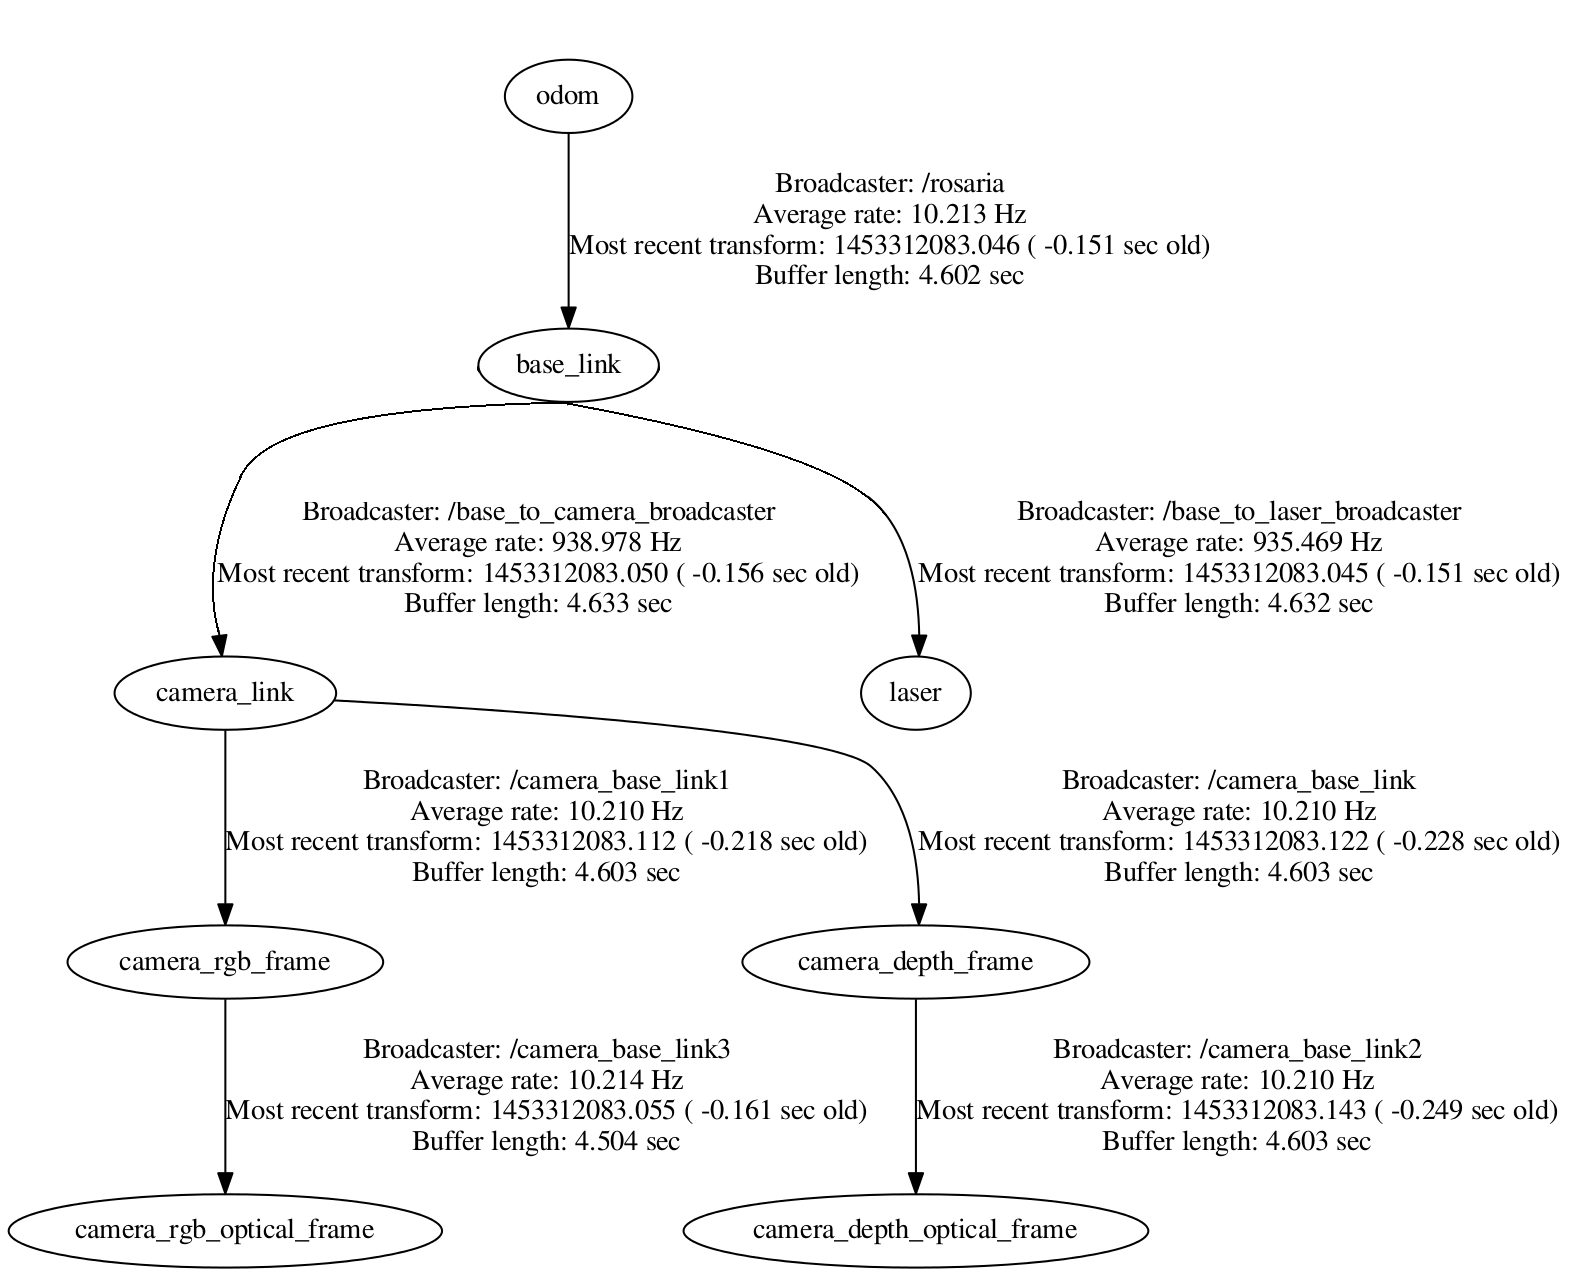
\includegraphics[width=0.8\textwidth]{figuras/frames-odom_base.png}
\caption{Referencias \textit{frames} de la configuraci�n del robot.}
\label{fig:frames-odom_base}
\end{figure}

\section{Nodo de teleoperaci�n}

Uno de los primeros objetivos de este proyecto es realizar el control teleoperado del robot. Utilizando ROS y sus caracter�sticas para operar de manera distribuida en diferentes m�quinas, esta tarea se vuelve inmediata para el usuario.

ROS trabaja en forma de procesos que se ejecutan de manera independiente y se comunican a trav�s del nodo principal o M�ster con el paso de mensajes. Ya que el m�ster dispone de una direcci�n IP en la m�quina que lo ejecuta, basta con indicar en el entorno ROS de cada m�quina la direcci�n de este para que los nodos abran una comunicaci�n con esa direcci�n IP.

Los pasos para configurar las m�quinas bajo la misma red se describen con detalle en la gu�a ROS NETWORKING y consisten b�sicamente en indicar en el sript \textit{.bashrc} el par�metro ROS	\_IP y ROS\_MASTER\_URI.

ROS\_IP debe contener la IP que tenga nuestra m�quina en la red que est� operando y ROS\_MASTER\_URI la direcci�n \textit{http} correspondiente de la m�quina donde se ejecute el nodo principal.

\begin{code}[htp]
\begin{lstlisting}[style=launch]
export ROS_IP=10.42.0.1
export ROS_MASTER_URI=http://10.42.0.1:11311
\end{lstlisting}
Fuente: \textit{$\sim$/.bashrc}
\caption{L�neas del archivo \textit{.bashrc} en el ordenador de abordo.}
\end{code}

\begin{code}[!htp]
\begin{lstlisting}[style=launch]
export ROS_IP=10.42.0.77
export ROS_MASTER_URI=http://10.42.0.1:11311
\end{lstlisting}
Fuente: $\sim$\textit{/.bashrc}
\caption{Ejemplo \textit{.bashrc} en un ordenador externo para realizar comunicaci�n con el m�ster.}
\end{code}

De esta manera podemos desarrollar un nodo ROS que se conecte al topic de RosAria que comanda los motores \textit{cmd\_vel} y publicar diferentes valores de velocidad en funci�n de las teclas que se pulsen.

\begin{code}[htp]
\begin{lstlisting}[style=C++]	
}
\end{lstlisting}
Fuente: $\sim$\textit{/.bashrc}
\caption{Ejemplo \textit{.bashrc} en un ordenador externo para realizar comunicaci�n con el m�ster.}
\end{code}

\begin{table}[!h]
\centering
\resizebox{\textwidth}{!}{
\begin{tabular}{c c c}
& {\bf teleop\_p3at API} & \\
{\bf Topics publicados} & {\bf Mensaje} & {\bf Descripci�n}\\ \hline
cmd\_vel & geometry\_msgs/Twist & Publica comandos de velocidad\\
\end{tabular}
}
\caption{API de teleop\_p3at}
\label{tabla:teleop_p3at}
\end{table}

\section{Nodo de navegaci�n estimada}

La navegaci�n estimada, m�s conocida en ingl�s como Dead Reckoning \cite{deadreckoning}, es la capacidad para realizar navegaci�n en un entorno bas�ndonos solamente en la informaci�n que aportan los sensores de la odometr�a.

Es un m�todo estimado de localizaci�n que se basa en la informaci�n de los encoders y no tiene en cuenta aspectos como el tipo de superficie, la inclinaci�n, el rozamiento o incluso obst�culos que puedan frenar o modificar el desplazamiento del robot (a pesar de que sus ruedas giren).

Este nodo de navegaci�n puede utilizarse para indicar al robot que avance cierta cantidad de metros y que realice giros a derecha o izquierda en un determinado �ngulo.

**Fragmento de c�digo**

\begin{table}[!h]
\centering
\resizebox{\textwidth}{!}{
\begin{tabular}{c c c}
& {\bf moving\_alone API} & \\
{\bf Topics suscritos} & {\bf Mensaje} & {\bf Descripci�n}\\ \hline
pose & nav\_msgs/Odometry & Recibe la odmetr�a\\
{\bf Topics publicados} & {\bf Mensaje} & {\bf Descripci�n}\\ \hline
cmd\_vel & geometry\_msgs/Twist & Publica comandos de velocidad\\
{\bf Frames suscritos} &  & {\bf Descripci�n}\\
\hline
base\_link & & Referencia base del robot\\
odom & & Referencia odom�trica
\end{tabular}
}
\caption{API de moving\_alone}
\label{tabla:moving_alone}
\end{table}

\chapter{Navegaci�n}\label{chapter:navegacion}

En este cap�tulo se expone el desarrollo referente a la navegaci�n dentro del ecosistema ROS. En �l se describen las caracter�sticas de navegaci�n del paquete de navegaci�n y sus posibilidades.

Este cap�tulo trata de abordar el aspecto de la navegaci�n desde el punto de vista de la utilidad, pasando por su fundamento te�rico y sin dejar de lado su aplicaci�n en el robot Pioneer 3 AT.

Por tanto, se exponen algunos ejemplos de configuraciones para la navegaci�n, sin embargo, la configuraci�n final del robot y la discusi�n sobre la misma se abordar� en el cap�tulo \ref{chapter:implementacion}, donde hablaremos de su implementaci�n m�s en detalle.

\section{Navigation Stack}
Dentro de las funcionalidades de ROS ya hemos comentado que existen los metapaquetes o "Stacks", que son grupos de paquetes de software que todos juntos ofrece una funcionalidad.

El paquete de navegaci�n de ROS \cite{navigation-ros} se define como un paquete de navegaci�n en dos dimensiones que toma informaci�n dela odometr�a, de los sensores y de un punto de meta y dirige el robot mediante comandos de velocidad seguros.

La navegaci�n se basa en el uso de "Mapas de coste'' y planificaci�n global y local de trayectorias.

Por un lado, el sistema hace un mapa de coste global que tiene encuentra informaci�n de los sensores y la posibilidad de cargar un mapa previo. A este mapa se incorporan los obst�culos que permanecen est�ticos durante m�s tiempo y en base a este se realizan los c�lculos de trayectoria global.

Por otro lado, el sistema realiza un mapa de coste local, que analiza los obst�culos m�s cercanos al robot en cada momento. A este mapa se incorpora la informaci�n de los sensores sobre cualquier tipo de obst�culo detectado. En base a este mapa se realizan los c�lculos de trayectoria local que llevar� el control de la navegaci�n reactiva del robot.

RELLENAR ALGO MAS

\subsection{Funcionamiento}

El paquete de navegaci�n se basa en diferentes nodos que interact�an para dirigir el robot hasta un punto en el mapa indicado como meta.

Este sistema utiliza un mapa de obst�culos est�ticos (global\_costmap), un mapa de obst�culo locales (local\_costmap), un nodo de c�lculo de trayectoria global (globa\_planner), un nodo de c�lculo de trayectoria local (local\_planner) y mecanismos de recuperaci�n de trayectoria (recovery\_behaviors).

\begin{figure}[!htp]
\centering
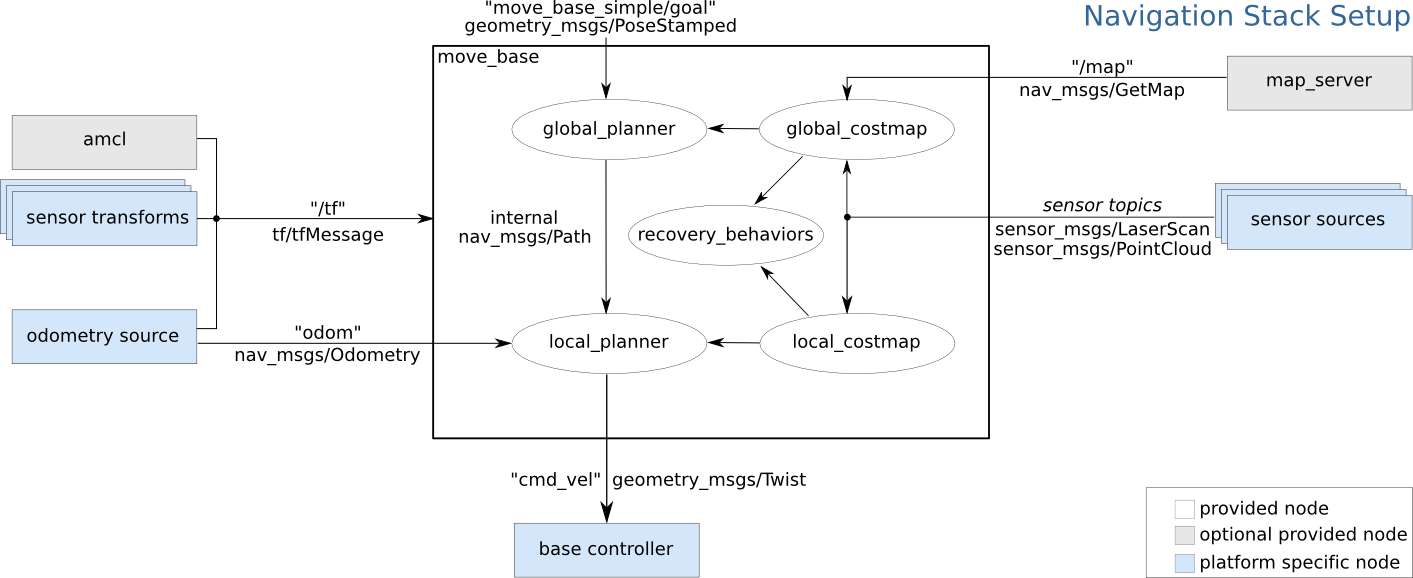
\includegraphics[width=\textwidth]{figuras/navigation-ros.png}
\caption{Diagrama de funcionamiento del Navigation Stack \cite{navigationsetup}}
\label{fig:navigation-ros}
\end{figure}

En el diagrama mostrado en la figura \ref{fig:navigation-ros} podemos ver una representaci�n de los nodos y mensajes utilizados por el paquete de navegaci�n as� como la informaci�n externa y opcional que se precisa.

Como puede apreciarse, los sensores, la odometr�a y el ajuste de las transfromadas entre cada uno de los sistemas de coordenadas son espec�ficos de cada plataforma rob�tica. La ejecuci�n principal se centra en el nodo \textit{move\_base} **referencia**, que es el ecargado de realizar los movimientos acorde a la informaci�n que aportan los mapas y los planificadores de trayectoria.

Por �ltimo indicar que el paquete de navegaci�n no precisa de un mapa pregrabado para funcionar. Puede utilizarse un mapa si se precisa y cargarlo mediante un nodo externo como \textit{map\_server} o generarlo simult�neamente a la navegaci�n mediante \textit{slam\_gmappig} (Subsecci�n \ref{subsection:slam_gmapping}).

El uso de un nodo de localizaci�n del robot en el mapa, como AMCL (Adaptive Monte Carlo Localization), ser� preciso cuando se utilice un mapa pregrabado para conocer la posici�n inicial del robot y posicionarlo correctamente dentro del mismo (Secci�n \ref{section:amcl}).

\subsection{Requisitos para la navegaci�n}
El sistema de navegaci�n de ROS est� dise�ado para ser flexible, altamente configurable y adaptable a muchos tipos de robots. Sin embargo requiere de ciertos requisitos para poder se integrado. A continuaci�n se describe cada uno de los requisitos aplicados al robot Pioneer 3 AT utilizado en este trabajo.

\textbf{Odometr�a}\\
El sistema de navegaci�n requiere de un robot que publique informaci�n sobre la odometr�a del robot en mensajes de tipo \textit{nav\_msgs/Odometry}.

En el robot Pioneer 3 AT y gracias al paquete RosAria (Subsecci�n \ref{subsection:rosaria}) obtenemos la informaci�n de los enconders del robot convertida en datos de odometr�a a trav�s del topic \textit{pose}.

\textbf{Movimientos}\\
El sistema de navegaci�n requiere que el robot sea controlable a trav�s de comandos de velocidad de tipo \textit{geometry\_msgs/Twist}.

En el robot Pioneer 3 AT y gracias al paquete RosAria (Subsecci�n \ref{subsection:rosaria}) podemos mover nuestro robot con comandos de velocidad publicandolos al topic \textit{cmd\_vel}.

\textbf{Sensores}\\
Los tipos de sensores que pueden utilizarse en la navegaci�n son variados, el requisito que deben cumplir para poder integrarse en el sistema de navegaci�n es que publiquen informaci�n de tipo \textit{sensor\_msgs/LaserScan} o \textit{sensor\_msgs/PointCloud2}.

Con los nodos descritos anteiormente, podemos obtener informaci�n de este tipo para el sensor Kinect (Subsecci�n \ref{subsection:kinect})y para el sensor L�ser (Subsecci�n \ref{subsection:sicklms100}). El nodo \textit{freenect\_stack} publica infomaci�n de la nube de puntos a trav�s del topic \textit{camera/depth/points} y el nodo \textit{LMS1xx} lo hace a trav�s del topic \textit{scan}.

\textbf{Transformadas}\\
Es necesario que toda la informaci�n est� estructurada geom�tricamente para que el sistema de navegaci�n pueda realizar los c�lculos pertinentes. Se requiere informaci�n de los sistemas de coordenadas de cada sensor, de la base del robot y de la odometr�a.

Cada uno de los nodos descritos con anterioridad publican diferentes \textit{frames} que sirven para este prop�sito. Estos \textit{frames} (\textit{odom, base\_link, laser, camera\_link}) relacionados mediante transformadas est�ticas como se describi� en la subsecci�n \ref{subsection:integracion_hardware}, proporcionan la informaci�n necesaria.

\subsection{Configuraci�n de la navegaci�n}
Hablar sobre los archivos necesarios .yaml y los launchfiles. de momento navegaci�n con mapa y explicaci�n.

Aunque se explicar� m�s adelante, una vez explicados los requisitos para utilizar el paquete de navegaci�n es necesario explicar cual es la configuraci�n necesaria para hacer que el sistema funcione.

En primer lugar, para facilitar la comprensi�n, suponemos que disponemos de un mapa del entorno en el que se va a desplazar nuestro robot y que disponemos de tan solo un sensor l�ser para realizar la navegaci�n.

Comenzamos por la configuraci�n de los llamados Costmaps, esto es, mapas que van almacenar los obst�culos del entorno del robot. Disponemos de global\_costmap y local\_costmap como dijimos antes y parte de la configuraci�n de estos ser� compartida, por tanto debemos crear un archivo de par�metros comunes \textit{costmap\_common\_params.yaml}.

\begin{code}[!htp]
\begin{lstlisting}[style=launch]
obstacle_range: 6.0
raytrace_range: 6.5
footprint: [ [0.254, -0.230], [-0.254, -0.230], [-0.254, 0.230], [0.254, 0.230] ]
inflation_radius: 0.5

observation_sources: laser_scan_sensor

laser_scan_sensor: {sensor_frame: laser, data_type: LaserScan, topic: /scan, marking: true, clearing: true}
\end{lstlisting}
\caption{Ejemplo de \textit{costmap\_common\_params.yaml}}
\end{code}

Como vemos, configuramos par�metros como la forma de nuestro robot, el radio de seguridad de los obst�culos, el rango de incorporaci�n de obst�culos y los sensores.

A continuaci�n creamos el archivo e configuraci�n de nuestro mapa global \textit{global\_costmap.yaml}.

\begin{code}[!htp]
\begin{lstlisting}[style=launch]
global_costmap:
  global_frame: /map
  robot_base_frame: base_link
  update_frequency: 5.0
  static_map: true
\end{lstlisting}
\caption{Ejemplo de \textit{global\_costmap.yaml}}
\end{code}

En este archivo vemos como este "mapa de coste" permanece est�tico y anclado al eje de coordenadas del mapa.

El mapa de navegaci�n local o reactiva es similar, aunque ne este caso el mapa tendr� unas dimensiones preestablecidas y se mover� con el robot.

\begin{code}[!htp]
\begin{lstlisting}[style=launch]
local_costmap:
  global_frame: odom
  robot_base_frame: base_link
  update_frequency: 5.0
  publish_frequency: 2.0
  static_map: false
  rolling_window: true
  width: 6.0
  height: 6.0
  resolution: 0.05
\end{lstlisting}
\caption{Ejemplo de \textit{local\_costmap.yaml}}
\end{code}

La configuraci�n b�sica del planificador local se guardar� en un archivo  \textit{base\_local\_planner\_params.yaml}.

\begin{code}[!htp]
\begin{lstlisting}[style=launch]
TrajectoryPlannerROS:
  max_vel_x: 0.45
  min_vel_x: 0.1
  max_vel_theta: 1.0
  min_in_place_vel_theta: 0.4

  acc_lim_theta: 3.2
  acc_lim_x: 2.5
  acc_lim_y: 2.5

  holonomic_robot: true
\end{lstlisting}
\caption{Ejemplo de \textit{local\_costmap.yaml}}
\end{code}

Tambi�n debemos indicar la configuraci�n del planificador global en \textit{global\_planner\_params.yaml}

\begin{code}[!htp]
\begin{lstlisting}[style=launch]
GlobalPlanner:
  old_navfn_behavior: false
  use_quadratic: true
  use_dijkstra: flase
  use_grid_path: false
\end{lstlisting}
\caption{Ejemplo de \textit{global\_planner\_params.yaml}}
\end{code}

Aqu� podemos definir el c�lculo de trayectorias siguiendo aproximaciones cuadr�ticas, basadas en ocupaci�n de celdas, tipo A* o Dijkstra (Se hablar� de cada una en la secci�n \ref{section:global_planner}).

Para finalizar, debemos ejecutar el nodo \textit{move\_base} con las configuraciones descritas anteriormente, as� como el mapa y el nodo de localizaci�n AMCL.

\begin{code}[!htp]
\begin{lstlisting}[style=launch]
<launch>
    <!-- Run the map server -->
    <node name="map_server" pkg="map_server" type="map_server" args="$(find pioneer_utils)/maps/floor_zero-map.yaml"/>

    <!--- Run AMCL -->
    <include file="$(find pioneer_utils)/navigation/common/amcl.launch"/>
	
	<node pkg="move_base" type="move_base" respawn="false" name="move_base" output="screen">
        <rosparam file="$(find pioneer_utils)/navigation/common/costmap_common_params_p3at.yaml" command="load" ns="global_costmap" />
        <rosparam file="$(find pioneer_utils)/navigation/common/costmap_common_params_p3at.yaml" command="load" ns="local_costmap" />
        <rosparam file="$(find pioneer_utils)/navigation/common/local_costmap_params.yaml" command="load" />
        <rosparam file="$(find pioneer_utils)/navigation/global_navigation/global_costmap_params.yaml" command="load" />
        <rosparam file="$(find pioneer_utils)/navigation/common/base_local_planner_params.yaml" command="load"/>
        <rosparam file="$(find pioneer_utils)/navigation/common/global_planner_params.yaml" command="load" />
    </node>
</launch>false
\end{lstlisting}
\caption{Ejemplo de \textit{robot\_navigation.launch}}
\end{code}

La representaci�n visual de ambos costmaps, el �rea del robot (footprint), el haz l�ser y el modelo de robot pueden observarse mediante RViz, tal y como muestra la figura \ref{fig:rviz_navigation}.

\begin{figure}[!htp]
\centering
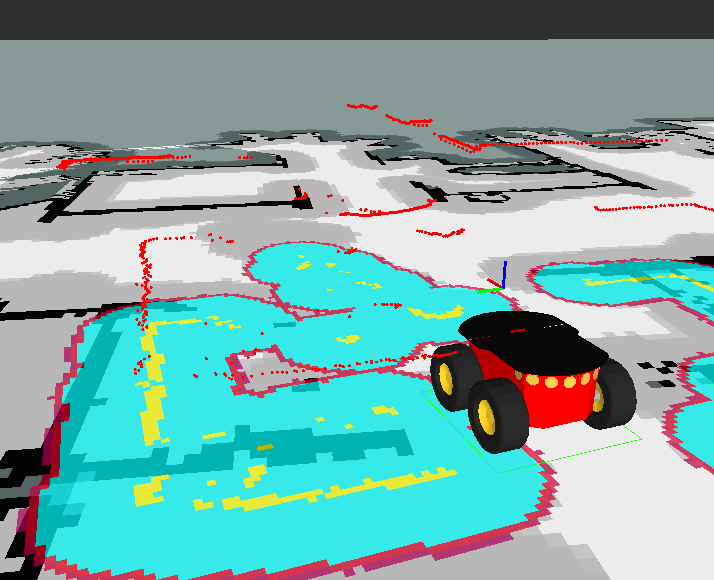
\includegraphics[width=0.8\textwidth]{figuras/rviz_navigation.png}
\caption{Visualizaci�n de costmaps, sensor l�ser y modelo del robot en RViz.}
\label{fig:rviz_navigation}
\end{figure}

Este primer ajuste no tiene en cuenta muchos factores concretos de la navegaci�n en el robot Pioneer 3 AT, como pueda ser la disposici�n correcta de los sensores, los ajustes de actualizaci�n de los mapas, el rango de los sensores o las interferencias de informaci�n que se incorporan o borran en los costmaps. Estos detalles se presentar�n en la implementaci�n del sistema (Cap�tulo \ref{chapter:implementacion}).

\section{SLAM}
La t�cnica de SLAM (Simultaneous Localization And Mapping) es una t�cnica muy utilizada en rob�tica para construir un mapa de un etorno que es desconocido al mismo tiempo que se estima la posici�n del robot en el mismo.

Esta t�cnica presenta dificultades como la imperfecci�n de los sensores, la imperfecci�n del sistema de locomoci�n el robot, la repetitividad de las medidas... Es por ello que se utilizan modos probabil�sticos como la relga de Bayes.

\begin{equation}
   p(x|d)=\frac{p(d|x)p(x)}{p(d)}
\end{equation}

\textbf{Principales algoritmos}\\
Los principales algoritmos para realizar los c�lculos pababil�sticos en t�cnicas de SLAM son los sigientes:

\begin{itemize}
\item Filtro extendido de Kalman: Es uno de los m�todos m�s extendidos en la t�cnica del SLAM por ofrecer resultados satisfactorios a pesar de sus problemas de estimaci�n \cite{rodriguez2006consistency}. Esta ha sido la t�cnica utilizada de facto hasta a aparici�n del FastSLAM \cite{montemerlo2002fastslam}.

\item Mapas de ocupaci�n de celdillas: Se basa en discretizar el espacio dividi�ndolo en unidades de tama�o predefinido que se clasifican como ocupadas o vac�as con un determinado nivel de confianza o probabilidad. La precisi�n (mayor cuanto m�s fina es la divisi�n del espacio), permite que el algoritmo de localizaci�n empleado acumule errores reducidos a lo largo de intervalos prolongados de tiempo. Su mayor desventaja de estos m�todos es la p�rdida de potencia que se deriva de no tener en cuenta la incertidumbre asociada a la posici�n del robot, lo cual origina que su capacidad para cerrar bucles correctamente se vea mermada \cite{collins2007occupancy}.
\end{itemize}

\subsubsection{slam\_gmapping en ROS}\label{subsection:slam_gmapping}
GMapping es una librer�a perteneciente al proyecto OpenSLAM \cite{openslam} que utiliza la t�cnica SLAM Grid Mapping, basada en la generaci�n de mapas mediante la ocupaci�n de celdillas utilizando un filtro de part�culas \cite{grisetti2007improved}.

En ROS se integra bajo el paquete gmapping \url{http://wiki.ros.org/gmapping} que no es m�s que un wrapper de OpenSLAM adaptando su interfaz.

Para crear mapas utilizando slam\_gampping precisamos de nuestro robot configurado para leer su odmetr�a un sensor capaz de ofrecernos informaci�n de tipo \textit{sensor\_msgs/LaserScan}.

En este caso nos servimos e la configuraci�n utilizada por el paquete \textit{p2os}:

\begin{code}[!htp]
\begin{lstlisting}[style=launch]
<launch>
	<node pkg="gmapping" type="slam_gmapping" name="slam_gmapping" args="/scan">
		<param name="delta" type="double" value="0.05" />
		<param name="temporalUpdate" type="double" value="2.5" />
		<param name="xmin" type="double" value="-2" />
		<param name="xmax" type="double" value="2" />
		<param name="ymin" type="double" value="-2" />
		<param name="ymax" type="double" value="2" />
	</node>
</launch>
\end{lstlisting}
\hypersetup{urlcolor=black}
Fuente: \href{https://github.com/allenh1/p2os/blob/indigo-stable/p2os_launch/launch/gmapping.launch}{\textit{p2os/p2os\_launch/launch/gmapping.launch}}
\hypersetup{urlcolor=blue}
\caption{Launchfile slam\_gmaping}
\end{code}

Para visualizar la creaci�n del mapa en RViz se ha creado un archivo espec�fico:

\begin{code}[!htp]
\begin{lstlisting}[style=consola]
$ roslaunch pioneer_utils rviz-gmapping.launch
\end{lstlisting}
\hypersetup{urlcolor=black}
Fuente: \href{https://github.com/danimtb/pioneer3at_ETSIDI/blob/master/pioneer_utils/rviz/rviz-gmapping.launch}{\textit{pioneer\_utils/rviz/rviz-gmapping.launch}}
\hypersetup{urlcolor=blue}
\caption{Launchfile para visualizar slam\_gmaping en RViz}
\end{code}

\begin{figure}[!htp]
\centering
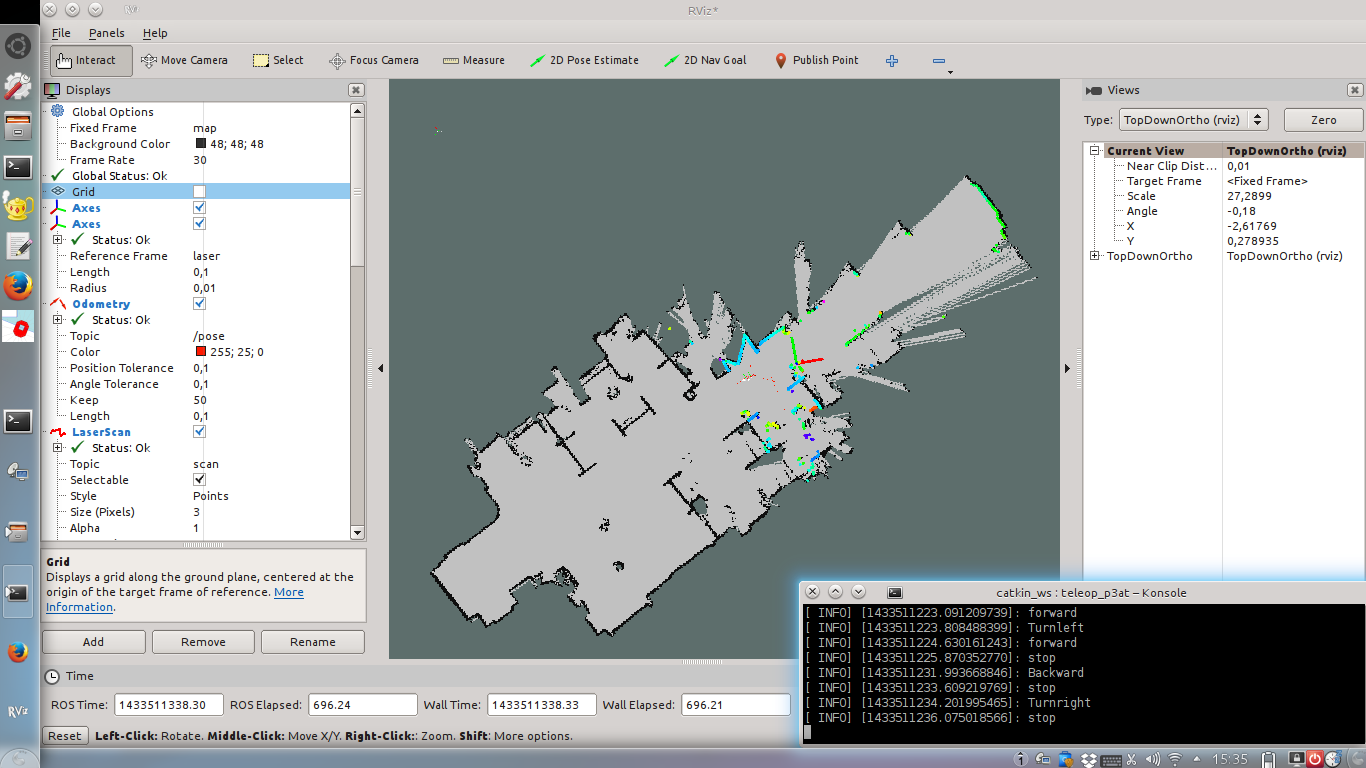
\includegraphics[width=0.8\textwidth]{figuras/pantalla_rviz_gmapping.png}
\caption{slam\_gmapping visualizado en RViz}
\label{fig:slam_gmapping_rviz}
\end{figure}

Finalmente, para guardar los mapas generados nos servimos de la herramienta map\_server que nos ofrece guardar mapas que se est�n publicando en el topic \textit{map} as� como publicar estos mapas para utilizarlos en la navegaci�n.

\begin{code}[!htp]
\begin{lstlisting}[style=consola]
$ rosrun map_server map_saver
\end{lstlisting}
\caption{Ejecuci�n del nodo map\_saver para guardar el mapa}
\end{code}

\section{AMCL}\label{section:amcl}
''Adaptative Monte Carlo Localizaion", tambi�n conocida por localizaci�n mediante filtro de part�culas, es un algoritmo utilizado en rob�tica para determinar la posici�n de un robot en un mapa \cite{fox1999monte}.

El algoritmo emplea un filtro de part�culas para representar una distribuci�n de posibles estados dentro del mapa. A medida que los sensores detectan el entorno y el robot se desplaza dentro de este se van otorgando mayor peso a aquellas part�culas que se encuentran m�s cercanas a la positic�n correcta y se van descartando otras.

La idea de esta t�cnica es conseguir que toas las part�culas converjan en una sola (a efectos pr�cticos, unas pocas part�culas) para determinar la posici�n del robot en el mapa.

Esta t�cnica se encuentra en ROS bajo un paquete llamado \textit{amcl} \cite{amcl-ros} y utiliza las t�cnicas descritas en el libro Probabilistic Robotics \cite{thrun2005probabilistic}.

Transladado a la filosof�a de funcionamiento de ROS, esta t�cnica nos ofrece la posibilidad de situar al robot en un mapa pregrabado, aport�ndonos la transformada entre el sistema de referencia (\textit{frame}) del mapa y el sistema de la odometr�a (Figura \ref{fig:amcl-ros}).

\begin{figure}[!htp]
\centering
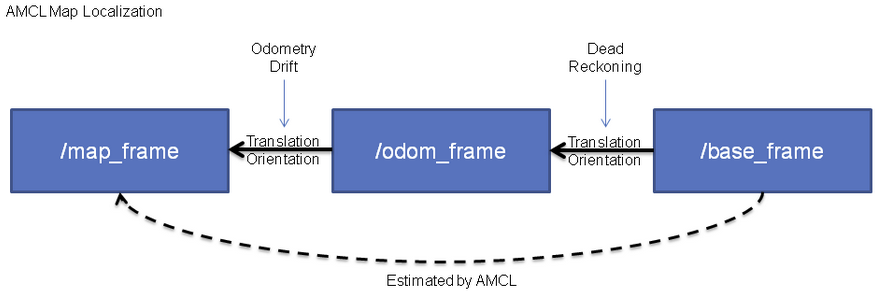
\includegraphics[width=0.9\textwidth]{figuras/amcl-ros.png}
\caption{Esquema de la labor del nodo AMCL entre los \textit{frames} map y base.}
\label{fig:amcl-ros}
\end{figure}

\textbf{Configuraci�n}

Como es habitual en ROS, esta funcionalidad nos aparece empaquetada en forma de nodo configurable a trav�s de par�metros.

Para funcionar requiere el uso de un mapa, el �rbol de transformadas de nuestro robot e informaci�n de tipo \textit{sensor\_msgs/LaserScan}.

La lista de par�metros configurables es amplia ya que debemos encontrar un modelo que se comporte bien con nuestro robot y sensor l�ser. Son especialmente importantes los par�metros del modelo de la odometr�a y los referentes al haz l�ser de nuestro sensor.

\begin{code}[!htp]
\begin{lstlisting}[style=launch]
<launch>
	<node pkg="amcl" type="amcl" name="amcl">
		<param name="odom_model_type" value="diff"/>
		<param name="odom_alpha5" value="0.1"/>
		<param name="transform_tolerance" value="0.2" />
		<param name="gui_publish_rate" value="10.0"/>
		<param name="laser_max_beams" value="30"/>
		<param name="min_particles" value="500"/>
		<param name="max_particles" value="5000"/>
		<param name="kld_err" value="0.05"/>
		<param name="kld_z" value="0.99"/>
		<param name="odom_alpha1" value="0.2"/>
		<param name="odom_alpha2" value="0.2"/>
		<param name="odom_alpha3" value="0.8"/>
		<param name="odom_alpha4" value="0.2"/>
		<param name="laser_z_hit" value="0.5"/>
		<param name="laser_z_short" value="0.05"/>
		<param name="laser_z_max" value="0.05"/>
		<param name="laser_z_rand" value="0.5"/>
		<param name="laser_sigma_hit" value="0.2"/>
		<param name="laser_lambda_short" value="0.1"/>
		<param name="laser_lambda_short" value="0.1"/>
		<param name="laser_model_type" value="likelihood_field"/>
		<param name="laser_likelihood_max_dist" value="2.0"/>
		<param name="update_min_d" value="0.2"/>
		<param name="update_min_a" value="0.5"/>
		<param name="odom_frame_id" value="odom"/>
		<param name="resample_interval" value="1"/>
		<param name="transform_tolerance" value="0.1"/>
		<param name="recovery_alpha_slow" value="0.0"/>
		<param name="recovery_alpha_fast" value="0.0"/>
	</node>
</launch>
\end{lstlisting}
\hypersetup{urlcolor=black}
Fuente: \href{https://github.com/danimtb/pioneer3at_ETSIDI/blob/master/pioneer_utils/navigation/common/amcl.launch}{\textit{pioneer\_utils/navigation/common/amcl.launch}}
\hypersetup{urlcolor=blue}
\caption{Launchfile del nodo amcl utilizado.}
\end{code}

\section{Mapas de coste: Costmaps}
Como ya se ha referido con anterioridad, el modelo de navegaci�n que sigue el Navigation Stack de ROS se basa en el concepto de Costmaps.

Un costmap es un mapa  generado a partir de los obst�culos detectados por sensores que son representados en forma de mapa de celdas y sobre los que se calcula un gradiente de "coste" desde los obst�culos hasta las zonas despejadas. Este tipo de mapas pretenden disponer de la informaci�n necesaria para que el robot pueda navegar.

Generalmente, este enfoque solo tiene en cuenta navegaci�n en un solo plano o navegaci�n en dos dimensiones, ya que todos los objetos son incorporados al mapa sin importar su altura. Existe una variante que pseudo-3D que tiene en cuenta la altura a la que se sit�an los sensores, aunque no es el modelo t�pico de aplicaci�n.

El funcionamiento de este tipo de mapas se basa en la incorporaci�n o el borrado de obst�culos al mapa. Cada sensor puede utilizarse de manera independiente para incorporar o borrar obst�culos en estos mapas. Esto permite a nuestro sistema rob�tico abstraerse de la informaci�n directa de los sensores y obtener informaci�n m�s completa de todos los obst�culos su alrededor.

La principal ventaja de utilizar este tipo de mapas en navegaci�n es la de crear mapas din�micos locales en el que guardar informaci�n de los obst�culos alrededor del robot sin que necesariamente dispongamos de un sensor captando el mismo continuamente. Esto nos permite, por ejemplo, realizar navegaci�n con un sensor con un rango horizontal de pocos grados, como el sensor Kinect, y a�n as� permitir al robot conocer informaci�n de obst�culos que han quedado fuera del rango del sensor.

El nodo encargado de la creaci�n de estos costmaps es \textit{costmap\_2d} y su funcionamiento est� basado en diferentes capas que manejan la infomraci�n de los sensores y generan c�lculos a partir de los mismos.

Las denominadas capas de las que hace uso \textit{costmap\_2d} son las siguientes:

\begin{itemize}
\item Satic Map: Esta capa es la encargada de tener el cuenta los obst�culos que aporta un mapa pregrabado en caso de utilizarse en la navegaci�n. Est� ligado al par�metro \textit{static\_map} y normalmente se utiliza con nodos de localizaci�n en un mapa como \textit{amcl}.

\item Obstacle Map: Esta capa es la encargada de incorporar o borrar obst�culos obteniendo la informaci�n de los sensores declarados en su archivo de configuraci�n. Destaca la facilidad para incorporar varios sensores a la vez.

\item Inflation: En esta capa se realizan los c�lculos de coste de cada celda a partir de la informaci�n que aportan las capas anteriores. Este gradiente de valores clasifica cada celda del mapa en diferentes tipos:

\begin{enumerate}[1.]
\item Letal: Existe un obst�culo real en esa celda del mapa
\item Inscrito: Las celdas con este valor se encuentran a una distancia de un obst�culo que es menor o igual al radio de la circunferencia inscrita en el �rea que ocupa el robot.
\item Posiblemente circunscrito: Celdas que se encuentran a una distancia de un obst�culo que es mayor que el radio de la circunferencia inscrita en el �rea que ocupa el robot pero menor que el radio de la circunferencia circunscrita. Esta informaci�n como "posible" debido que la orientaci�n del robot puede no ser exacta.
\item Espacio libre: El coste de este tipo de celdas es cero e indica que no existe ningun obst�culo cercano que impida o limite el movimiento del robot.
\item Desconocido: No existe informaci�n sobre el estado de esa celda.

\end{enumerate}

\begin{figure}[!htp]
\centering
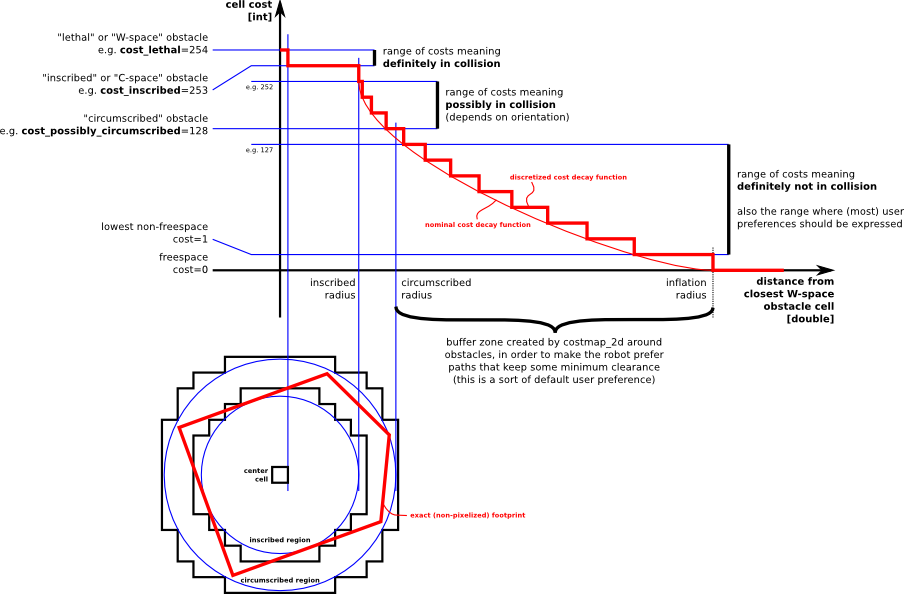
\includegraphics[width=\textwidth]{figuras/inflation_layer.png}
\caption{Esquema sobre el c�lculo del coste de cada celda en el mapa.}
\label{fig:inflation_layer}
\end{figure}

Esta capa indica a los planeadores las zonas optimas por las que trazar su ruta, es la m�s importante y donde reside gran parte de la funcionalidad de los costmaps. Existen par�metros configurables por el usuario como el radio de inflado (\textit{inflation\_radius}) o el valor de escala (\textit{cost\_scaling\_factor}).
\end{itemize}

A parte de estas capas, existe una API que nos permite crear nuestras propias capas para el nodo \textit{costmap\_2d} para darles la funcionalidad que se desee.

Existe una configuraci�n por defecto que de estos costmaps que genera una sola capa de obst�culos, una capa de inflado y adcionalmente una capa de mapa est�tico siempre y cuando pongamos el par�metro \textit{static\_map} a TRUE. Sin embargo, existe la posibilidad de crear costmaps con las capas que consideremos oportunas, siendo de especial inter�s poder incorporar diferentes capas de obst�culos.

Este �ltimo enfoque es el que ha sido adoptado en la implementaci�n final de navegaci�n y ser� descrito en el apartado **APARTADO**.

\section{Planificador de trayectoria global}\label{section:global_planner}
La planificaci�n de trayectoria es una de las �reas que m�s inter�s suscita entre los investigadores relacionados con la rob�tica m�vil o la navegaci�n aut�noma, no en vano, existe una gran variedad de algoritmos que realizan c�lculos apoy�ndose en distintos enfoques matem�ticos.

Los planificadores de trayectoria tratan de construir o planificar la ruta que lleve al robot desde su posici�n a un punto en un mapa o en un entorno que pudiera ser desconocido. Esta planificaci�n es calculada en un �mbito que denominamos "global" ya que se realiza en funci�n al mapa global (\textit{global\_costmap} en nuestro caso) y no se condideran los detalles del entorno local al robot. Es, por tanto, una aproximaci�n al camino final que el robot va a seguir.

**texto de transici�n**

A continuaci�n vamos a describir los planificadores de trayectoria disponibles en ROS, su fundamento te�rico y su comportamiento en el c�culo de la trayectoria.

Standard (Dijstra??)
grid\_path
simple potential
A*
navfn
TEOR�A
ALGORITMOS CON PRUEBAS
PLANIFICADOR FINAL

\section{Planificador de trayectoria local}
Resolver las obstrucciones sobre la ruta global en el
entorno local al robot para determinar la ruta real que ser� seguida. El modelo del entorno local se construye mediante la fusi�n de la informaci�n proporcionada por los sensores externos del robot m�vil.

TEOR�A
FUNCIONAMIENTO
VALORACI�N DE SEGUIMIENTO DE TRAYECTORIA GLOBAL
PLANIFICADOR FINAL

\chapter{Implementaci�n del sistema}\label{chapter:implementacion}

Este cap�tulo describe los cambios, ajustes y modificaciones que, basados en la informaci�n anterior expuesta, las caracter�sticas de ROS y el hardware del que disponemos, se han realizado para alcanzar los objetivos del proyecto.

\section{Configuraciones hardware}
Como ya se ha descrito, la navegaci�n se basa en el sensor Kinect pero tambi�n se ha considerado integrar el sensor l�ser debido a la valiosa informaci�n que aporta y su disponibilidad.

Por ello, el robot deber� llevar incorporados estos sensores proporcion�ndoles alimentaci�n y una interfaz de conexi�n adecuada.

\subsection{Pioneer 3 AT}
El robot Pioneer 3 AT de Adept Mobile Robots es la base de la plataforma rob�tica. El modelo disponible en el laborarotio de la Escuela T�cnica Superior de Ingenier�a y Dise�o Industrial llevaba incorporado un ordenador de tipo **ORDENADOR PIONEER**. Tambi�n, al comienzo de este proyecto ya exist�an algunas adaptaciones como la incorporaci�n de un altavoz frontal, acceso a los puestos USB del ordenador interno y conexi�n para el sensor l�ser.

IMAGEN ROBOT ESTADO INICIAL.

El robot hab�a sido utilizado anteriormente mediante el software MRCore en el proyecto **PROYECTO DE ALEJANDRO** y el sistema operativo del ordenador interno era Ubuntu Server 10.

Para integrar la versi�n Indigo de ROS lo m�s recomendable era partir de la versi�n estable m�s actualizada de Ubuntu, por lo que se sustituy� el sistema operativo por Ubuntu 14.04 LTS en su versi�n de escritorio.

Una vez integrado el sistema operativo, la primera toma de contacto con el robot fue a partir de la librer�a Aria **referencia** para controlar el movimiento de los motores y comprobar que el robot se encontraba en buen estado.

**A�adir el puerto al grupo de dialout**

A continuaci�n, tras instalar ROS Indigo, se procedi� a las pruebas mediante el paquete Rosaria de ROS. La conexi�n con el microcontrolador de la placa de motores fue exitosa y se comprob� que los valores de la odometr�a tambi�n funcionaban.

**cambiar el puerto de conexion*?*


Llegados a este punto, ya dispon�amos del robot preparado para realizar las primeras pruebas.

\subsection{Sensor L�ser}
El sensor l�ser Sick ya hab�a sido integrado en un proyecto anterior y sus conexiones de alimentaci�n y datos v�a Ethernet ya estaban preparadas para utilizarlo.

Para conectarlo a trav�s del puerto Ethernet fue necesario ajustar su direcci�n IP a trav�s del software del fabricante y ajustar la IP del ordenador del robot Pioneer (m�s informaci�n en el ap�ndice **TAL**).

El agarre mec�nico del sensor se dej� tal y como hab�a sido utilizado en ocasiones anteriores, situado en la parte frontal agarrado mediante un par de tornillos al chasis con tuercas de palometa para su f�cil manipulaci�n.

**Imagen del sensor l�ser en el robot**.

El sensor l�ser se conecta a la interfaz ROS mediante el paquete LMS1xx tal y como se describi� en el apartado \ref{subsection:sicklms100}.

\subsection{Sensor Kinect}
La integraci�n del sensor Kinect fue relativamente sencilla debido a que las entradas de los puestos USB del ordenador hab�an sido cableadas previamente. La adaptaci�n a realizar era sobre la parte de alimentaci�n, ya que este sensor trabaja a una tensi�n de 12 voltios.

En el manual del robot se encuentra una descripci�n detallada de la placa de alimentaci�n a la cual pueden conectarse diferentes perif�ricos. Esta placa ofrece tomas de conexi�n de 5 voltios controlados por unos botones auxiliares y tomas de 12 voltios (ver ap�ndice **TAL**).

El sensor Kinect dispone de un adaptador USB, preparado para trabajar con la videoconsola XBOX 360, el cual suministra 12 voltios mediante un transformador conectado a una toma de corriente alterna de 220v e incorpora los cables de datos del propio sensor Kinect.

**Esquema conexion usual**.

Para integrar el sensor Kinect en el robot, se cort� el cable de alimentaci�n del cable adaptador y se soldaron unas clavijas tipo Jack **REVISAR** macho-hembra para conectar el adaptador directamente a los 12 voltios de la placa del robot. Tambi�n se realiza� lo oportuno en el adaptador de corriente, para poder usar el sensor Kinect de la manera habitual.

**Imagen de los componentes**

Para anclar el sensor Kinect al robot se opt� por situarlo en la parte superior del sensor L�ser, para lo cual se dise�� una pieza que encajase en la base de la Kinect y en el sensor l�ser (figura **REF**).

**Imagen del dise�o 3D**

El sensor Kinect se conecta a la interfaz ROS mediante el paquete freenect\_stack tal y como se describi� en el apartado \ref{subsection:kinect}.

\subsection{Primera configuraci�n hardware}
La primera configuraci�n del robot consisti� en ambos sensores situados en la parte frontal del mismo. Ambos sensores de encontraba uno encima del otro, de tal forma que no existieran interferencias entre uno y otro.

**Imagen del robot**

\subsubsection{Primera configuraci�n del sistema}
El ordenador interno corr�a todos los nodos de ROS, de modo que se dispon�a de la informaci�n de los sensores, el control sobre los motores y la lectura de la odometr�a para realizar las primeras pruebas con el paquete de navegaci�n de ROS (Secci�n \label{section:navigation_stack}).

Sin embargo, la primera implementaci�n con los primeros ajustes a nuestro hardware de los sensores no fue posible debido a la sobrecarga de la CPU del ordenador interno del robot Pioneer y a problemas de memoria en la ejecuci�n de nodos como AMCL.

\subsubsection{Segunda configuraci�n del sistema}
La siguiente opci�n fue utilizar un ordenador externo que realizase los c�lculos de navegaci�n y enviase al robot las consignas de movimiento a trav�s de una red WLAN. Esta idea no era la soluci�n m�s ideal, ya que desde el principio la idea era que el robot fuese lo m�s aut�nomo posible sin depender de una infraestructura, sin embargo era una posibilidad directa que no supon�a mucho esfuerzo.

**esquema configuraci�n**

Gracias a la filosof�a de ejecuci�n distribuida de nodos de ROS, ejecutar nodos en m�quinas diferentes y compartir la informaci�n entre procesos es una tarea sencilla. Para configurarlo, tan solo es necesario indicar a las m�quinas la IP del nodo master. De esta forma, los nodos que se ejecuten en cada una de las m�quinas tratar�n de realizar la comunicaci�n a trav�s de IPs dentro de la misma red.

Este ajuste fue puesto en marcha utilizando un ordenador port�til con suficiente capacidad de procesamiento y memoria como para ejecutar la navegaci�n, sin embargo aparecieron algunos inconvenientes.

El primero de ellos fueron las direcciones IP en el ordenador interno del Pioneer.

\textbf{Problemas con el sensor L�ser: LM1xx}\\
Debido a que el sensor l�ser se conecta v�a Ethernet a este ordenador, el nodo LMS1xx debe obtener informaci�n a trav�s de la IP del l�ser y enviarla a trav�s del adaptador Wifi a la IP del nodo m�ster. El problema resid�a en que el nodo se saturaba al tener que lidiar con ambas interfaces de conexi�n y provocaba su detenci�n.

Tras varias consultas a Clearpath Robotics a trav�s de su repositorio de GitHub y preguntas en el foro ROS Answers **Enlaces de referencia**, la soluci�n no estaba implementada en c�digo y lo m�s inmediato era hacer un bridge en el ordenador del Pioneer 3 AT entre la interfaz Ethernet y la Wifi.

Los resultados de esta soluci�n no fueron satisfactorios ya que el comportamiento era el mismo: el nodo LMS1xx se saturaba e interrump�a a los pocos minutos de su ejecuci�n.

Trantando de resolver este problema, se hicieron pruebas generando una red Wifi Ad-hoc desde el ordenador del robot, a la cual se conectaba el ordenador externo. Los resultados fueron buenos siempre y cuando las IPs del nodo master y del sensor L�ser se encontrasen en el mismo subrango **revisar nomenclatura**.

En la implementaci�n final del sistema esta soluci�n se sigue utilizando para conectarse desde un ordenador externo al ordenador que incorpora el robot Pioneer.

**OJOOOO continua seccion**

Una vez se pudo conectar el ordenador externo, la ejecuci�n del nodo de navegaci�n era la correcta y las consignas de movimiento se enviaban correctamente al robot, pudiendo realizar las primeras pruebas de navegaci�n aut�noma.

**Imagen primeras navegaciones**

Sin embargo en ocasiones la recepci�n y env�o de datos era demasiado alta y esto provocaba que existiese mucho retraso en la comunicaci�n, haciendo que el robot reaccionase tarde para esquivar los obst�culos y el control del robot fuera impracticable.

\subsubsection{Tercera configuraci�n del sistema}
Finalmente se opt� por montar un ordenador m�s potente en el robot, para lo cual se utiliz� un port�til externo al que se conectaba tanto e sensor Kinect como el sensor L�ser y se utilizaba un convertidor de puesto USB a puerto serie RS-232 para controlar el movimiento del robot y leer la odometr�a. El ordenador del robot quedaba sustituido y as� se mantuvo hasta la versi�n final.

**imagen del robot con el port�til**

Llegados a este punto, ahora s� dispon�amos de la plataforma rob�tica completa sobre la que trabajar en la navegaci�n del robot. Las primeras pruebas fueron satisfactorias, logrando correr todos los nodos en el port�til, el cual se incorpor� de manera provisional al robot por medio de unos agarres realizados con una impresora 3D.

**imagen de los agarres**

\subsection{Segunda configuraci�n}

La segunda configuraci�n hardware vino dada tras las pruebas satisfactorias con l
\subsubsection{Configuraci�n del sistema final}
\textbf{Intel NUC}

\section{Navegaci�n}
\subsection{Sensores}
\subsection{Navegaci�n con mapa}
\subsection{Navegaci�n reactiva}
\section{Nodo de navegaci�n por puntos}
\section{Nodo de comandos por voz}
\subsection{Reconocimiento de comandos de voz}
\subsection{Feedback mediante text-to-speech}

\section{Nodo de ejecuci�n autom�tica de nodos}


\chapter{Pruebas del sistema}
En este cap�tulo se describen las principales pruebas realizadas con el robot de tal modo que sirva para validar el trabajo realizado y exponer los resultados obtenidos.

Dividimos este cap�tulo en dos partes, pruebas del robot en simulaci�n y pruebas en el entorno real, centr�ndonos exclusivamente en la creaci�n de mapas mediante SLAM y los tests de navegaci�n por ser el objeto principal de este proyecto.

\section{Pruebas simuladas}
En este apartado se describen las pruebas llevadas a cabo en el simulador Gazebo con el modelo del robot descrito anteriormente. Cabe indicar que todas las pruebas se realizan con la misma configuraci�n que en el caso del robot real a excepci�n de los nodos de bajo nivel.

\subsection{SLAM}
Las pruebas de SLAM se realizaron con el ya mencionado nodo \textit{slam\_gmapping}, funcionando de la manera habitual.

Para comprobar su validez, se dispuso al robot en el mundo "Willow Garage" que simula un entorno de oficinas, similar al entorno real del laboratorio. El objetivo principal fue comprobar que el algoritmo de mapeado funcionaba correctamente y que se consegu�a cerrar el mapa realizando un bucle completo.

Para esta prueba se utiliz� el nodo de mapeado y el de teleoperaci�n y se gui� al robot por una parte del entorno realizando diversos bucles (Figura \ref{fig:slam_gazebo}), en los que se observa que no existe distorsi�n en paredes paralelas y que el mapa no se encuentra solapado.

\begin{figure}[!htp]
\centering
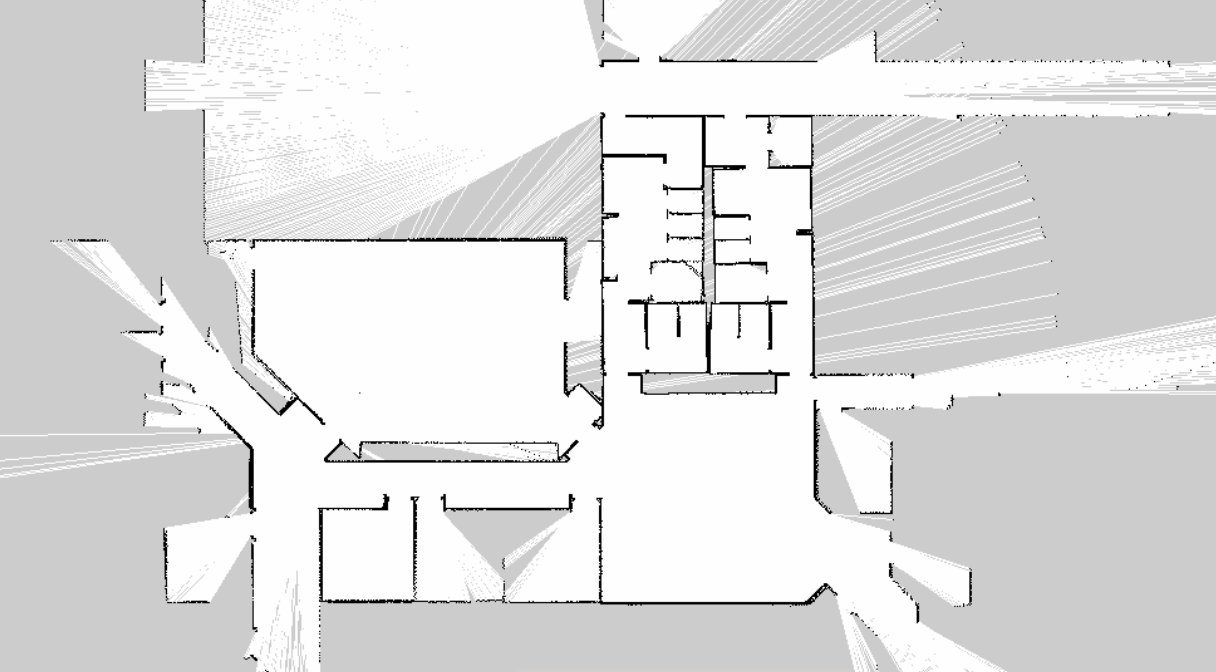
\includegraphics[width=0.8\textwidth]{figuras/slam_gazebo.png}
\caption{Prueba de SLAM en el simulador Gazebo.}
\label{fig:slam_gazebo}
\end{figure}

Indicar que este fue el mapa base utilizado para la navegaci�n de sucesivas pruebas con Gazebo en las cuales el nodo AMCL situ� correctamente al robot en el entorno virtual, por lo que validaci�n del mapa generado es correcta.

\subsection{Navegaci�n con mapa}
Las navegaciones con mapa en el simulador fueron determinantes para realizar una configuraci�n m�s elaborada de ambos costmaps debido a los problemas con el borrado de los obst�culos (ver Subsecci�n \ref{subsection:configuracion_costmaps_sensores}).

En un principio se valor� la posibilidad de utilizar el sensor Kinect tan solo para obst�culos locales y el sensor l�ser para obst�culos globales, sin embargo esta idea se descart� ya que el robot trataba de seguir una trayectoria global incorrecta que no contemplaba los obst�culos bajos (Figura \label{fig:discrepancia_costmaps_gazebo}), con las complicaciones de control que eso supone para el planificador de trayectoria local.

\begin{figure}[!htp]
\centering
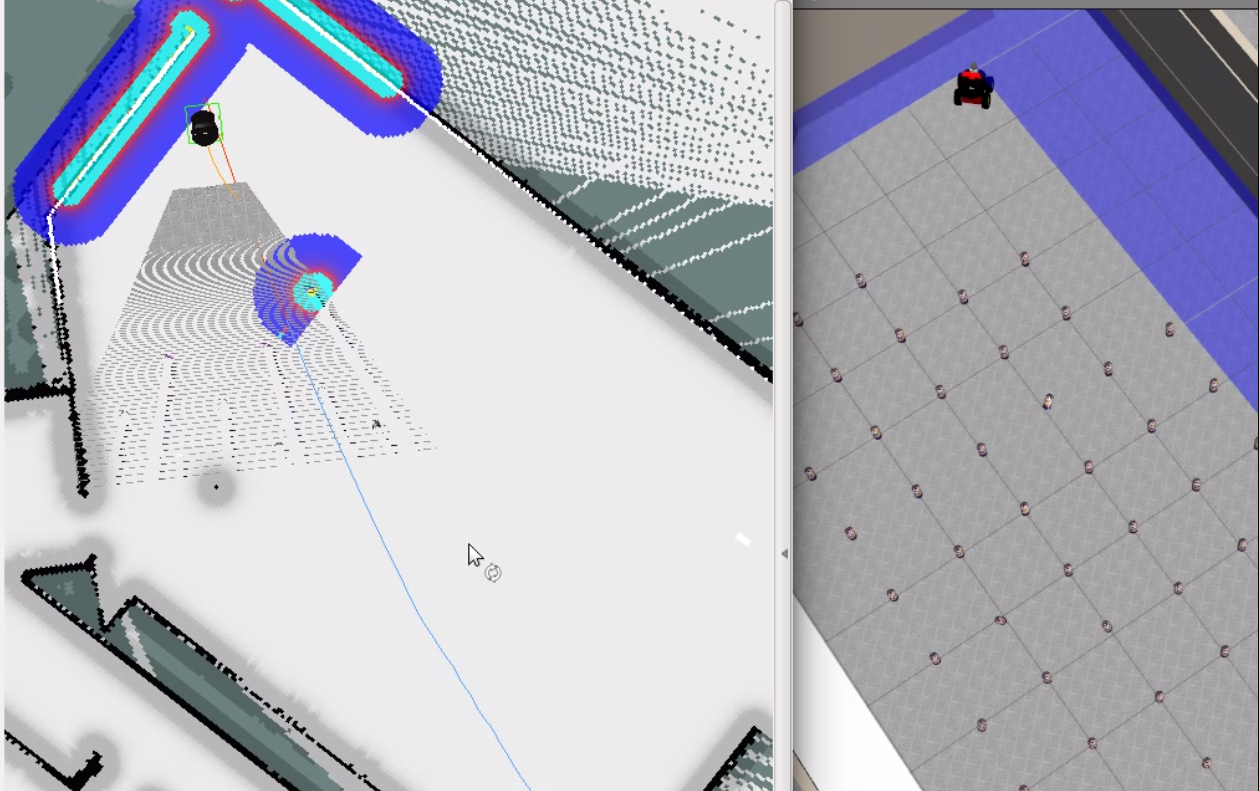
\includegraphics[width=0.65\textwidth]{figuras/discrepancia_costmaps_gazebo.png}
\caption{Trayectoria global erronea.}
\label{fig:discrepancia_costmaps_gazebo}
\end{figure}

Esto determin�, junto con las caracter�sticas especiales del sensor Kinect, que los sensores fueran recolocados para la configuraci�n final del robot y que se a�adiesen capas de obst�culos diferenciadas para cada sensor.

Pruebas posteriores con la nueva configuraci�n y obst�culos bajos determinaron la configuraci�n correcta. Adem�s se configur� un c�lculo de trayectoria global repetitivo (par�metro \textit{planner\_frequency: 1.0}), de tal modo que el planificador global genera trayectorias actualizadas a medida que el robot se desplaya e incorpora nuevos obst�culos al mapa. Esto ayuda al planificador local de trayectoria y en definitiva a que el robot realice menos maniobras.

\begin{figure}[!htp]
\centering
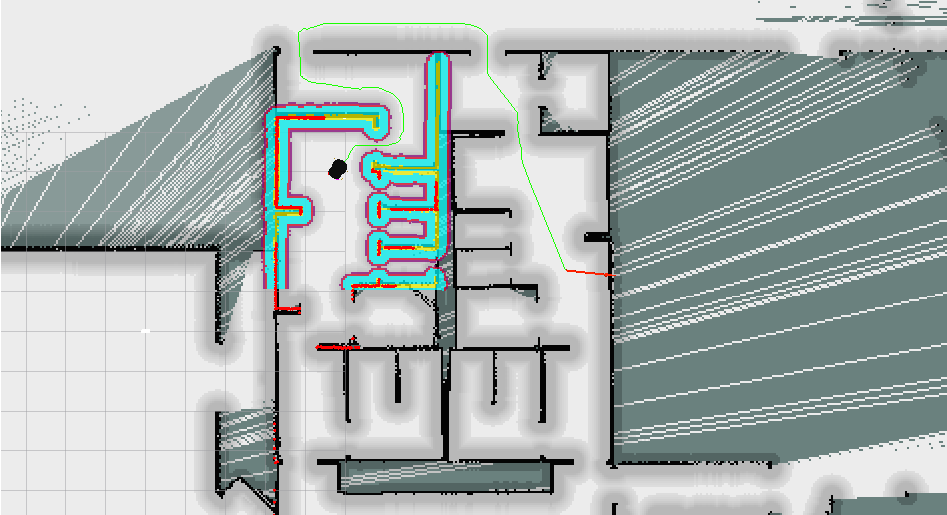
\includegraphics[width=0.7\textwidth]{figuras/navegacion_global_gazebo.png}
\caption{Navegaci�n con mapa final.}
\label{fig:navegacion_global_gazebo}
\end{figure}

\subsection{Navegaci�n reactiva}
La nagaci�n reactiva es una configuraci�n menor de la anterior, por lo que no supuso un desarrollo m�s elaborado en las pruebas realizadas. Las pruebas consistieron en realizar navegaci�n hacia varios puntos de meta y comprobar si el robot se quedaba atascado en alg�n momento.

Los resultados determinaron que el robot mostraba el mismo comportamiento en la navegaci�n pero exist�an limitaciones como la distancia a la que pueden encontrarse los puntos de meta (puntos m�s cercanos al robot debido a la ausencia de mapa) o solapamientos y giros en el mapa global si este era demasiado grande.

Como es normal en una navegaci�n reactiva, el robot se desplaza siguiendo la trayectoria m�s corta en base a la informaci�n que sus sensores captan en ese momento, por lo que suceden casos, como en la figura \label{fig:navegacion_local_gazebo}, en los que la trayectoria global calculada no es la correcta en un principio. A pesar de ello, gracias a la informaci�n de los obst�culos que queda retenida en el mapa global, el planificador recalcula encontrando la trayectoria adecuada.

\begin{figure}[!htp]
\centering
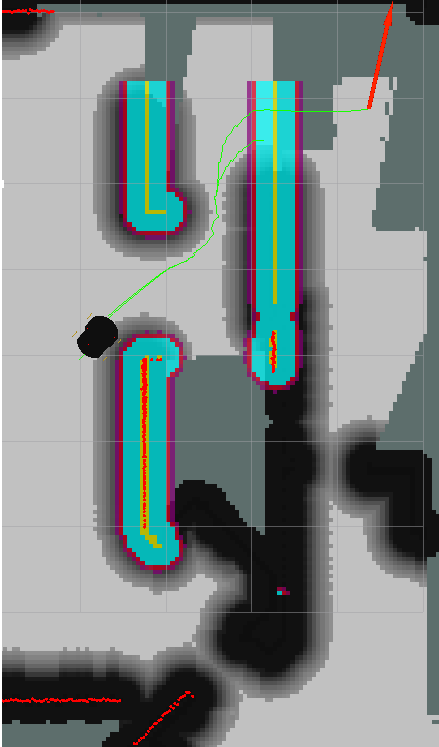
\includegraphics[width=0.30\textwidth]{figuras/navegacion_local1_gazebop.png}
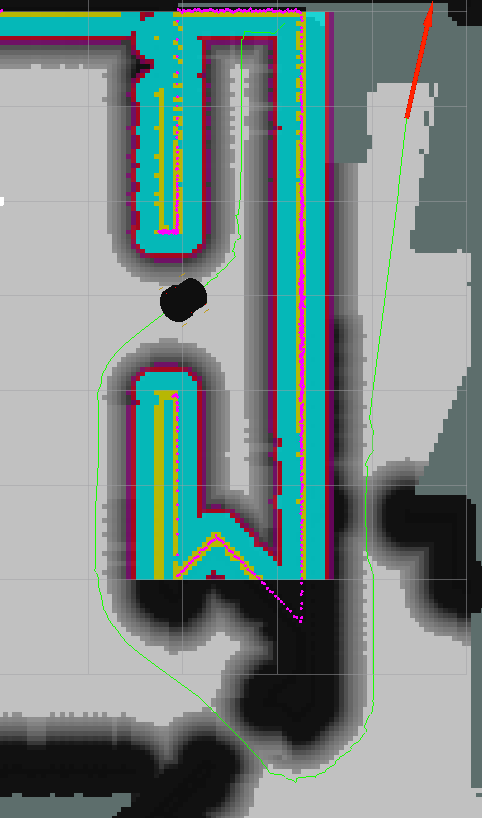
\includegraphics[width=0.30\textwidth]{figuras/navegacion_local2_gazebop.png}
\caption{Navegaci�n con mapa final.}
\label{fig:navegacion_local_gazebo}
\end{figure}

\subsection{Pruebas de resistencia}
Para las pruebas de resistencia utilizamos un nodo \textit{endurance\_test}, espec�ficamente creado para el caso.

En estas pruebas se consideraron las siguientes variables:
\begin{itemize}
\item Puntos de meta: Puntos totales repartidos por el mapa que serviran como puntos objetivo a alcanzar por el robot.
\item Tiempo total: Tiempo total de la prueba.
\item Metas enviadas: N�mero total de puntos de meta que se han enviado como objetivo al robot durante la prueba.
\item Metas alcanzadas: N�mero de metas a las que ha conseguido llegar el robot.
\item Tasa de metas alcanzadas: Tanto por ciento de las metas alcanzadas respecto de las enviadas.
\item Distancia total: Distancia total recorrida, considerando obst�culos intermedios y maniobras o replanificaci�n de trayectorias del robot.
\item N� de choques: N�mero de obst�culos con los que el robot ha chocado (si los hubiera).
\end{itemize}

Las pruebas de resistencia se realizaron en el modo de navegaci�n con mapa, el entorno virtual fue el mundo "Willow Garage" y se utilizaron un total de 9 puntos de meta como objetivo, distribuidos de manera aleatoria (dentro de habitaciones, pasillos, salas grandes...) a distancias largas. Cabe se�alar que no existe ning�n tipo de obst�culo m�vil implicado en estas pruebas.

\textbf{Primera prueba}\\
Prueba inicial sin obst�culos adicionales en el entorno.

\begin{table}[!h]
\centering
\resizebox{0.5\textwidth}{!}{
\begin{tabular}{c c}
\hline
Puntos de meta &  9 \\
Tiempo total & 20 minutos \\
Metas enviadas & 18 \\
Metas alcanzadas & 18 \\
Tasa metas alcanzadas & 100\% \\
Distancia total & 275.2 metros \\
N� de choques & 0 \\
\hline
\end{tabular}
}
\caption{Primera prueba de resistencia simulada.}
\label{tabla:primera_prueba_simulada}
\end{table}
La navegaci�n del robot fue correcta durante toda la prueba.

\pagebreak

\textbf{Segunda prueba}\\
Segunda prueba m�s larga y con obst�culos adicionales en el entorno.

\begin{table}[!h]
\centering
\resizebox{0.5\textwidth}{!}{
\begin{tabular}{c c}
\hline
Puntos de meta &  9 \\
Tiempo total & 56 minutos \\
Metas enviadas & 29 \\
Metas alcanzadas & 22 \\
Tasa metas alcanzadas & 75\% \\
Distancia total & 354.6 metros \\
N� de choques & 0 \\
\hline
\end{tabular}
}
\caption{Segunda prueba de resistencia simulada.}
\label{tabla:segunda_prueba_simulada}
\end{table}
La prueba finaliz� debido a que el robot qued� inmobilizado por encontrarse demasiado cerca de una pared frontal y otra lateral. El incremento de tiempo a pesar de no haber recorrido muchos m�s metros respecto de la prueba anterior se debe a las esperas por reintento en alcanzar las metas fallidas.

A pesar de todo el robot no colisiona con ning�n obst�culo.

\textbf{Tercera prueba}\\
Tercera prueba con las mismas caracter�sticas que la anterior. El objetivo de esta prueba era recorrer una distancia total m�s larga sin colisi�n.

\begin{table}[!h]
\centering
\resizebox{0.5\textwidth}{!}{
\begin{tabular}{c c}
\hline
Puntos de meta &  9 \\
Tiempo total & 23 minutos \\
Metas enviadas & 18 \\
Metas alcanzadas & 15 \\
Tasa metas alcanzadas & 83\% \\
Distancia total & 488.8 metros \\
N� de choques & 0 \\
\hline
\end{tabular}
}
\caption{Tercera prueba de resistencia simulada.}
\label{tabla:tercera_prueba_simulada}
\end{table}
Las metas no alcanzadas se produjeron por un exceso de tiempo en alcanzarlas, saltando el \textit{timeout} y abortando la meta objetivo.

Los resultados de esta prueba indican que los planificadores responden bien en el c�lculo de trayectorias hacia puntos de meta alejados.

\section{Pruebas reales}
Las pruebas reales se llevaron a cabo en el robot con su configuraci�n hardware y configuraci�n del sistema final. Todos los nodos se ejecutan en el ordenador integrado Intel NUC y se utiliza un ordenador cliente para visualizar datos o teleoperar el robot en caso necesario.

Las pruebas de navegaci�n con y sin mapa se han omitido debido a que los resultados fueron correctos y no se observaron grandes diferencias respecto a los resultados obtenidos en el simulador.

\subsection{SLAM}
Las pruebas reales de SLAM se realiazron en la planta baja y el aparcamiento de la universidad, ya que era de los pocos lugares donde pod�a realizar un bucle completo.

Para realizar estas pruebas se utiliz� al robot en modo de guiado y al mismo tiempo se realiz� el mapeado. Indicar que no existen interferencias al realizar SLAM guiando de este modo al robot, ya que la persona que sirve de gu�a se encuentra en frente y solo es detectada por el sensor Kinect, de tal modo que el sensor l�ser se encarga de mapear el entorno sin perturbaciones.

En la figura \ref{fig:slam_real1} se muestra el resultado de la primera prueba.

\begin{figure}[!htp]
\centering
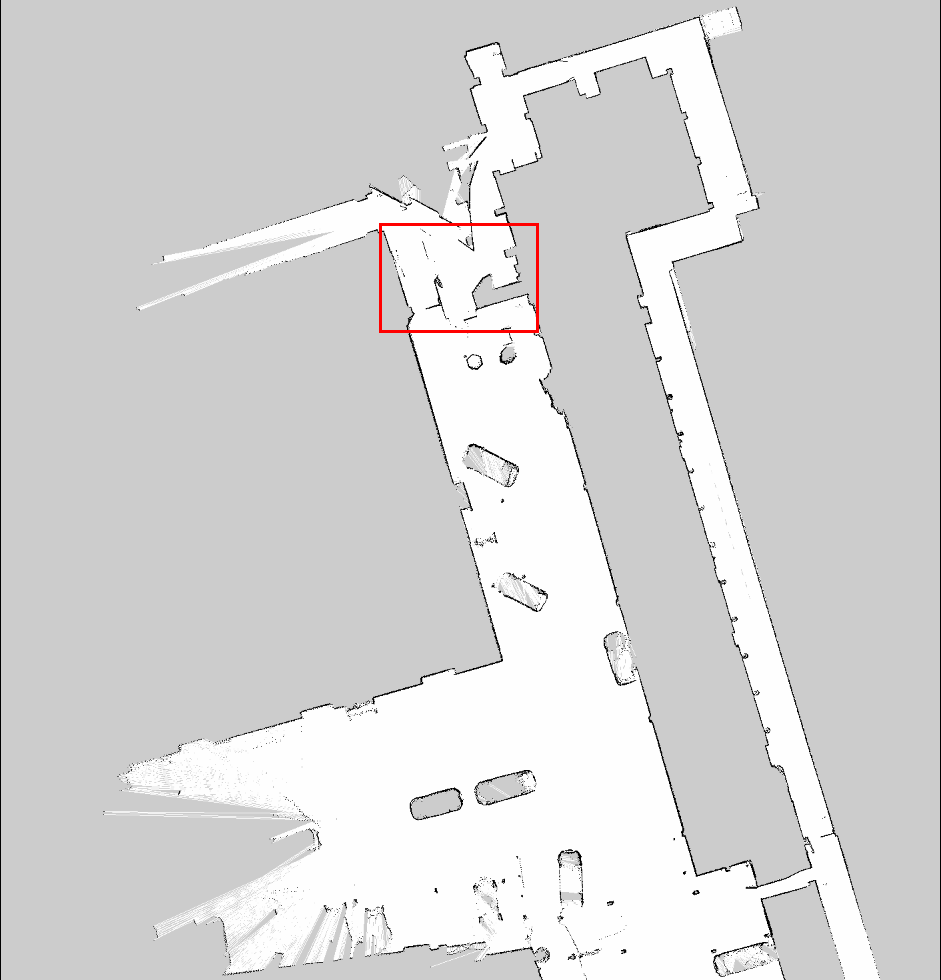
\includegraphics[width=0.9\textwidth]{figuras/slam_real1.png}
\caption{Mapa con la primera prueba de SLAM.}
\label{fig:slam_real1}
\end{figure}
\footnotemark
\footnotetext{\hypersetup{urlcolor=black}
Fuente: \href{https://github.com/danimtb/pioneer3at_ETSIDI/blob/master/pioneer_utils/maps/slam_real1.pgm}{\textit{pioneer\_utils/maps/slam\_real1.pgm}}
\hypersetup{urlcolor=blue}}

El �rea recuadrada en color rojo indica la zona de cierre del bucle, donde se aprecian ciertas discrepancias en las paredes y un ligero desv�o hacia la derecha. Parte de este efecto es debido a que el bucle a cerrar es demasiado grande para esta prueba y a que el robot se desplaz� realizando un recorrido sinuoso por el �rea del parking (se aprecia que se cubri� gran parte del mismo sin ser algo necesario para la prueba), con lo que el error de la odometr�a pudo haberse visto incrementado.

Debido a estos resultados se decidi� realizar una segunda prueba de SLAM en las mismas condiciones pero guiando al robot de una manera m�s directa a lo largo del bucle (sin giros adicionales).

En la figura \ref{fig:slam_real2} puede apreciarse el resultado de la segunda prueba con el cierre del bucle en la zona recuadrada en rojo. Esta vez el resultado es mejor, ya que no existen grandes discrepancias y el robot es capaz de situarse sin problemas. Tan solo se aprecia una pared exterior duplicada en �ngulo, fruto ligero desv�o en el mapa.

\begin{figure}[!htp]
\centering
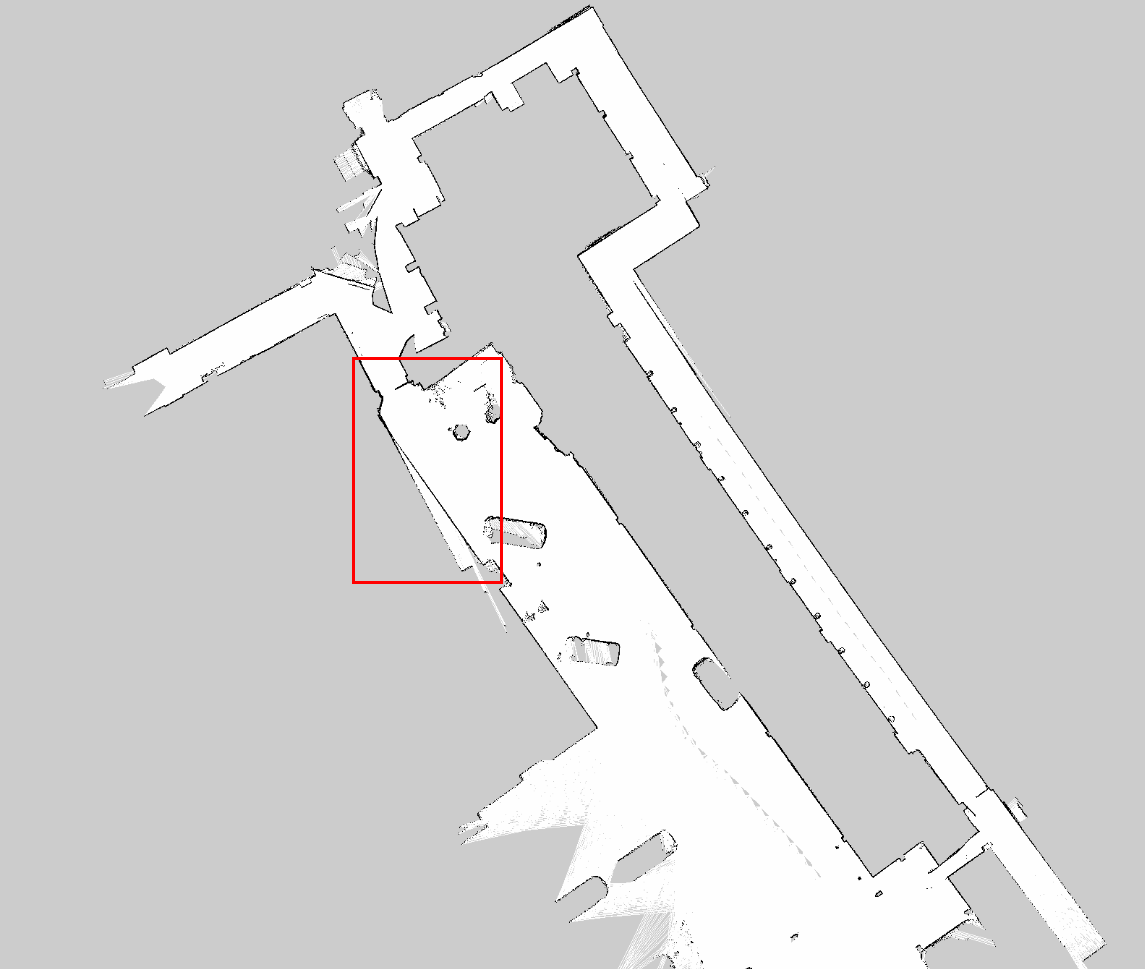
\includegraphics[width=\textwidth]{figuras/slam_real2.png}
\caption{Mapa tras la segunda prueba de SLAM.}
\label{fig:slam_real2}
\end{figure}
\footnotemark
\footnotetext{\hypersetup{urlcolor=black}
Fuente: \href{https://github.com/danimtb/pioneer3at_ETSIDI/blob/master/pioneer_utils/maps/slam_real1.pgm}{\textit{pioneer\_utils/maps/slam\_real1.pgm}}
\hypersetup{urlcolor=blue}}

\subsection{Pruebas de resistencia}
Las pruebas de resistencia se llevaron a cabo en las instalaciones de la planta baja de la universidad mediante el nodo \textit{endurance\_test} creado para el caso y utilizando diversos puntos dentro del mapa "floor\_zero-map"\footnote{\hypersetup{urlcolor=black}Fuente: \href{https://github.com/danimtb/pioneer3at_ETSIDI/blob/master/pioneer_utils/maps/floor_zero-map.pgm}{\textit{pioneer\_utils/maps/floor\_zero-map.pgm}}
\hypersetup{urlcolor=blue}} que abarca las zonas indicadas.

El objetivo primordial de las pruebas es que el robot sea capaz de navegar sin ning�n tipo de intervenci�n humana, ya que invalidar�a el concepto de robot aut�nomo.

\textbf{Primera prueba}\\
Primera prueba real desarrollada en el laboratorio con obst�culos y personas en movimiento.

\begin{table}[!h]
\centering
\resizebox{0.5\textwidth}{!}{
\begin{tabular}{c c}
\hline
Puntos de meta &  7 \\
Tiempo total & 44 minutos \\
Metas enviadas & 91 \\
Metas alcanzadas & 56 \\
Tasa metas alcanzadas & 61\% \\
Distancia total & - \\
N� de choques & 0 \\
\hline
\end{tabular}
}
\caption{Primera prueba de resistencia real\protect\footnotemark.}
\label{tabla:primera_prueba_real}
\end{table}
\footnotetext{La distancia total recorrida no pudo contabilizarse debido a un error en la configuraci�n del nodo.}

Los resultados de la primera prueba no reflejan una navegaci�n buena del robot, sin embargo esto es debido a la existencia de obst�culos prominentes no incluidos en el mapa del laboratorio que generaban distorsi�n en AMCL provocando que el robot quedase mal situado en el mapa. Estos obst�culos generaban a su vez un pasillo estrecho a trav�s del cu�l el planificador en ocasiones no era capaz de trazar una trayectoria correcta hasta la meta.

A pesar de ello el robot no colision� con ning�n tipo de obst�culo.

\textbf{Segunda prueba}\\
Segunda prueba de mayor recorrido, con obst�culos adicionales en el entorno y personas en movimiento. El objetivo de la prueba era medir la total movilidad del robot en el laboratorio.

\begin{table}[!h]
\centering
\resizebox{0.5\textwidth}{!}{
\begin{tabular}{c c}
\hline
Puntos de meta &  7 \\
Tiempo total & 57 minutos \\
Metas enviadas & 141 \\
Metas alcanzadas & 114 \\
Tasa metas alcanzadas & 80\% \\
Distancia total & 1119.5 metros \\
N� de choques & 4 \\
\hline
\end{tabular}
}
\caption{Segunda prueba de resistencia real.}
\label{tabla:segunda_prueba_real}
\end{table}
La prueba finaliz� por falta de bater�a en el robot, sin embargo no puede considerarse que ese tiempo sea la duraci�n de la misma en navegaci�n con el robot ya que no se encontraba al 100\%.

Las metas no alcanzadas se produjeron por obst�culos m�viles (personas en movimiento) bloqueando el paso del robot (imposible llegar a la meta f�sicamente). Tambi�n se produjeron metas abordadas por riesgo de colisi�n (el robot hab�a quedado situado muy cerca de las patas de una mesa).

Los choques fueron roces leves de las ruedas con obst�culos bajos. Esto es debido a que el planificador ajusta mucho la trayectoria para que el robot pueda navegar por lugares estrechos.

Cabe destacar la distancia total recorrida, que asciende a m�s de un kil�metro realizando maniobras con todo tipo de obst�culos.

\textbf{Tercera prueba}\\
La tercera prueba de resistencia se plante� como la prueba absoluta, midiendo par�metros como la autonom�a de las bater�as, con distancias entre puntos m�s largas, navegaci�n por diferentes salas y peque�os desniveles.

Los puntos de meta preestablecidos se distribuyen en el mapa tal y como se muestra en la figura \ref{fig:endurance_real2} y el robot navega aleatoriamente de uno a otro.

\begin{figure}[!htp]
\centering
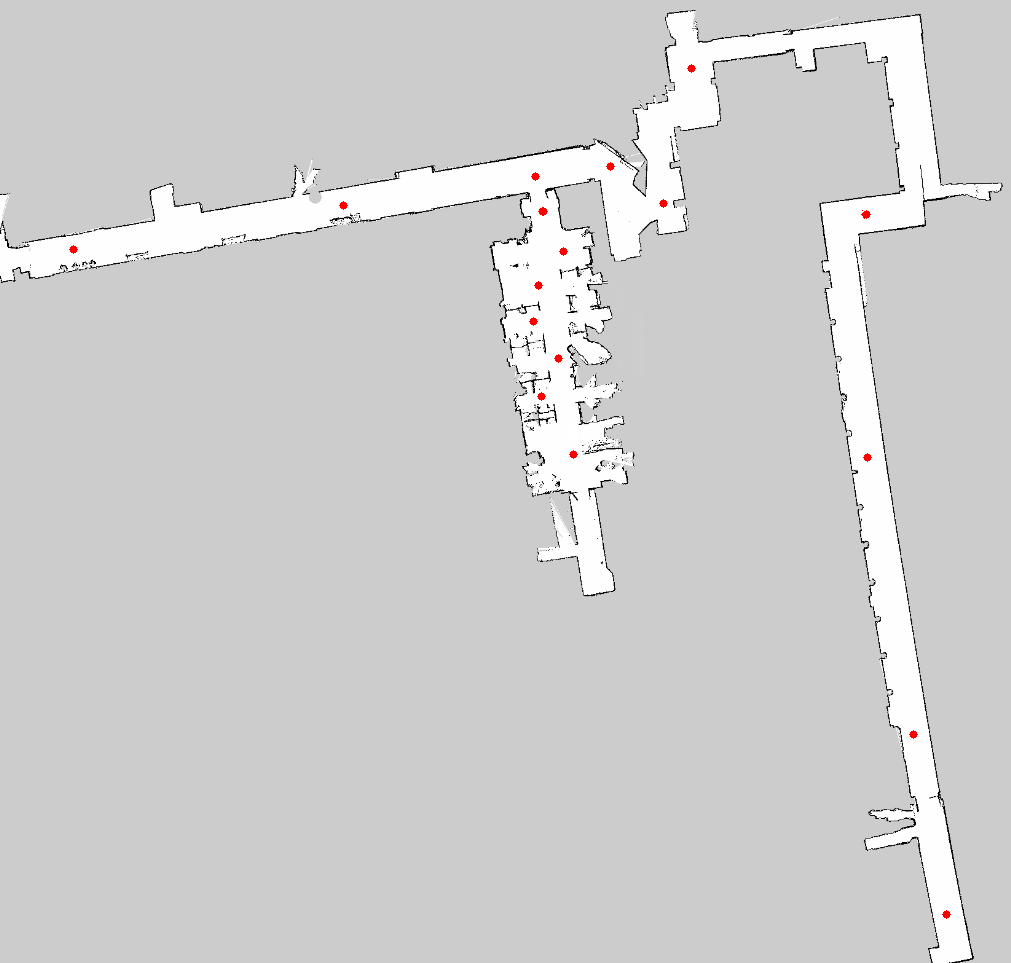
\includegraphics[width=0.8\textwidth]{figuras/mapa_endurance.png}
\caption{Distribuci�n de puntos de meta en la segunda prueba de resistencia.}
\label{fig:endurance_real2}
\end{figure}

El entorno de la prueba present� obst�culos altos y bajos (no detectables por el sensor l�ser), dos peque�as rampas, personas en continuo movimiento e incluso elementos del entorno cambiados de posici�n. A continuaci�n se muestran los resultados de la prueba.

\begin{table}[!h]
\centering
\resizebox{0.5\textwidth}{!}{
\begin{tabular}{c c}
\hline
Puntos de meta &  17 \\
Tiempo total & 2 horas y 38 minutos \\
Metas enviadas & 164 \\
Metas alcanzadas & 106 \\
Tasa metas alcanzadas & 65\% \\
Distancia total & 4000.5 metros \\
N� de choques & 2 \\
\hline
\end{tabular}
}
\caption{Tercera prueba de resistencia real.}
\label{tabla:tercera_prueba_real}
\end{table}

Sobre estos resultados cabe decir que el n�mero de metas alcanzadas se ve reducido debido a que en ocasiones el planificador global precisaba de alg�n reintento para trazar la taryectoria al el punto de meta y a que el robot a veces encontraba dificultades para conducir su trayectoria a trav�s de pasos estrechos.

La duraci�n de la bater�a en navegaci�n continua durante esta prueba super� las dos horas y media. Al finalizar la prueba el voltaje de las bater�as alcanz� un valor 10.5 voltios.

En cuanto al n�mero de choques, estos fueron un roce a un obst�culo bajo al tratar de esquivarlo y un choque con las ruedas de una silla.

Destaca el alto valor de la distancia recorrida, que alcanza los 4 kil�metros sin la intervenci�n humana, sin que se ponga en riesgo la integridad de ninguna persona involucrada en la prueba ni la del propio robot.

\subsection{Ascpectos de la navegaci�n}

Tras las pruebas realizadas, analizando los resultados y observando el comportamiento general de todo el sistema rob�tico podemos decir que existen algunas limitaciones en la navegaci�n y aspectos que no se tienen en cuenta por las caracter�sticas del robot.

\begin{itemize}
\item \textbf{En cuanto a la navegaci�n:}\\
Existen limitaciones en cuanto a rampas, ya que este modo de navegaci�n no tiene en cuenta la inclinaci�n del robot para saber si este se encuentra desplaz�ndose por un plano inclinado. Por otro lado tampoco es posible distinguir cambios por debajo del plano de navegaci�n como agujeros, escalones... Estos dos aspectos se deben principalmente a que la navegaci�n se realiza puramente en dos dimensiones.

No obstante, el sistema s� es capaz de absorber peque�as rampas en las que los sensores no reciban excesivas interferencias con el cambio de plano y siempre que el robot no realice muchos giros para no comprometer la localizaci�n debido al cambio del rozamiento de las ruedas del robot con el suelo.

\item \textbf{En cuanto a las caracter�sticas del robot:}\\
Ciertos obst�culos bajos no son detectados por los sensores debido a que el robot es capaz de superarlos sin problemas, es por ello que no se ha incidido en detectarlos.

Obst�culos de materiales transparentes, como puertas de cristal, no son detectadas por ninguno de los dos sensores debido a su naturaleza infrarroja, por tanto se definen este tipo de obst�culos como caso l�mite para el sistema rob�tico.
\end{itemize}



\chapter{Conclusiones}

En este apartado se presentan las conclusiones del estado actual del proyecto y algunos desarrollos que podr�an implementarse como mejoras del mismo.

\section{Conclusi�n}
Una vez finalizado el proyecto se puede afirmar que los objetivos iniciales han sido cumplidos.
El objetivo de familiarizarse con e entorno rob�tico ROS se ha superado, adquiriendo considerables conocimientos de variedad t�cnicas que conciernen a la puesta a punto del sistema y a su aplicaci�n a los robots m�viles en particular.

Tambi�n ha sido llevada a cabo la integraci�n de los sensores l�ser y Kinect dentro del sistema rob�tico de tal forma que se detectan obst�culos del entorno en dos y tres dimensiones.

Se ha cumplido con el objetivo del desarrollo de un sistema de teleoperaci�n para el robot, as� como otras aplicaciones menores que aportan valor al sistema rob�tico como la navegaci�n basada en la odometr�a o el guiado del robot mediante personas, lo cual supone una caracter�stica a�adida en la interacci�n con el robot.

El sistema de navegaci�n aut�noma y orientaci�n se han realizado de manera satisfactoria, en gran parte debido a la optimizaci�n realizada en la distribuci�n de los sensores, el correcto tratado de la informaci�n sensorial, el adecuado ajuste de los mapas y de sus respectivos planificadores de trayectoria. Si bien es cierto que existen algunos aspectos que la navegaci�n actual no cubre, como la posibilidad de encontrar cambios de plano en la superficie, esto no impide que el robot pueda absorber variaciones del mismo sin comprometer el sistema de navegaci�n utilizado.

Adicionalmente se han desarrollado nuevas funcionalidades como la navegaci�n por puntos, la interacci�n mediante comandos de voz, la reproducci�n de sonidos y sintetizado de voz adem�s de la puesta en marcha del simulador rob�tico Gazebo.

Por �ltimo, todos los objetivos anteriores han servido para que la integraci�n de los elementos implicados en este proyecto formen parte de la plataforma m�vil final, de tal modo que su funcionamiento a bajo nivel quede solventado de cara a futuros desarrollos. Los resultados obtenidos en las pruebas de resistencia reflejan el buen comportamiento del robot en entornos reales y que el sistema es completamente funcional.

\section{Desarrollos futuros}

A continuaci�n se analizar�n algunos desarrollos y aspectos a afrontar en futuros
trabajos que tengan como objeto mejorar el sistema propuesto.

\subsection{Navegaci�n en tres dimensiones}
Durante este proyecto se ha abordado la navegaci�n bas�ndose en un �nico plano de tal modo que el an�lisis del entorno queda reducido a dos dimensiones. El uso de Kinect como sensor en tres dimensiones considera ciertos obst�culos a alturas diferentes por lo que puede considerarse que la navegaci�n implementada es pseudo-3D. En cualquier caso, la reducci�n de los obst�culos a una sola capa restringe el movimiento del robot de manera vertical (al subir una cuesta por ejemplo) por lo que lo m�s adecuado ser�a implementar un sistema de navegaci�n que considerase el entorno en 3 dimensiones.

Este posible desarrollo aportar�a ventajas en cuanto a las capacidades del robot, ya que podr�an considerarse adecuadamente cambios de inclinaci�n en la superficie de navegaci�n as� como detectar huecos o agujeros en el suelo por los que la marcha del robot ser�a impracticable. Esto conlleva en primer lugar a que el sistema rob�tico deba estar dotado de una referencia de posici�n en el eje vertical para que puedan detectarse desplazamientos en una superficie inclinada. Esto podr�a realizarse con el inclin�metro incorporado en el sensor Kinect u otro sensor adicional de mayor precisi�n.

En segundo lugar, la captura del entorno debe realizarse tambi�n tres dimensiones de tal modo que puedan obtenerse mapas que el robot pueda tomar de referencia. La estimaci�n de su posici�n en el mismo tambi�n ser�a uno de los aspectos a considerar.

Por �ltimo habr�a que utilizar planificadores de trayectoria en tres dimensiones teniendo en cuenta la particularidad de que el robot debe permanecer situado siempre en un plano de apoyo.

La capacidad para navegar considerando un entorno tridimensional real aportar�a al robot grandes posibilidades para abordar terrenos irregulares, desniveles o elementos comunes en interiores como peque�os escalones y rampas. Una posible implementacion ser�a utilizar el paquete \textit{3d\_navigation} de ROS.

\subsection{Sens�rica adicional embebida}
En relaci�n con el desarrollo propuesto anteriormente, incorporar nuevos sensores al sistema rob�tico supondr�a una ventaja por varias razones.

En primer lugar, considerar la inclinaci�n del robot mediante aceler�metros para realizar una navegaci�n en tres dimensiones aportar�a m�s libertad de movimientos al robot y lo dotar�a del conocimiento real de su posici�n y orientaci�n.

En segundo lugar, incorporar sensores esteroceptivos de naturaleza distinta al haz infrarrojo permitir�a detectar obst�culos transparentes como puertas de cristal o mamparas, elementos comunes en entornos interiores. Sensores de ultrasonidos colocados en puntos estrat�gicos y a diferente altura har�an que el sistema considerase este tipo de elementos, aumentando las capacidades del mismo.

Otros sensores esteroceptivos podr�an estar orientados a la detecci�n de desniveles inminentes, de tal modo que el robot no pudiese caer en caso de encontrarse pr�ximo al borde. Esto ser�a interesante en un entorno con escaleras por ejemplo.

En tercer lugar, podr�a ser interesante incorporar sensores de posicionamiento absoluto tanto para interiores como para exteriores. En el caso de entornos interiores, esta tarea es m�s compleja debido a que ser�a necesario utilizar un sistema de balizas o similar que formase parte de la infraestructura. Sin embargo, incorporar un sistema GPS aportar�a gran valor al robot en exteriores sin que suponga un alto esfuerzo de desarrollo.

Para la incorporaci�n de futuros sensores tambi�n podr�a considerarse realizar un sistema de adquisici�n de datos a trav�s de puerto USB e implementar su interfaz en ROS. Esto supondr�a dotar al robot de una interfaz de conexi�n gen�rica para toda una variedad de sensores adicionales.

Indicar que este posible desarrollo deber�a tener en cuenta la fusi�n sensorial de los datos para que no existan duplicidades o perturbaciones en la percepci�n del entorno del robot.

\subsection{Interacci�n con el robot}
Los puntos adicionales incluidos en este proyecto como el guiado del robot mediante seguimiento de personas, el reconocimiento de �rdenes por voz o el feedback mediante sonidos y voz han servido para evaluar la interacci�n de las personas con el mismo.

El uso de un robot para navegaci�n en interiores hace de la interacci�n con personas un aspecto fundamental, por lo que implementar nuevas formas de interactuar con el mismo dota de mucho valor en cuanto a facilidad de uso y capacidades como robot social.

El desarrollo futuro en esta �rea puede ser considerable debido a que las posibilidades de interacci�n pueden venir dadas mediante instrucciones de voz, determinados gestos o movimientos captados mediante visi�n artificial, navegaci�n sem�ntica, etc.

En concreto, una de las funcionalidades a mejorar ser�a el seguimiento de personas ya que actualmente el sistema se encuentra restringido a una detecci�n b�sica de un objeto situado frente al robot, por lo que si la distancia al mismo es demasiado grande el robot no es capaz de mantener la distancia. Esto podr�a mejorarse utilizando referencias visuales que permitiesen al robot reproducir la trayectoria realizada por una persona que realice la funci�n de gu�a.


\appendix
\addappheadtotoc
\appendixpage
\chapter{Configuraci�n del sistema} \label{chapter:configuracion_sistema}

En este ap�ndice se resume de manera simplificada y muy enfocada la configuraci�n completa del sistema rob�tico objeto de este trabajo, tanto la parte referente al software de robot como la parte destinada a la configuraci�n hardware de todos los equipos que incorpora.

\section{Configuraci�n del espacio de trabajo}
En ROS el espacio de trabajo es el lugar donde se realiza el desarrollo software de los paquetes ROS. Este en torno de trabajo es capaz de gestionar la correcta compilaci�n de los nodos.

El espacio de trabajo es el determinado por la herramienta Catkin. A partir de la versi�n Indigo de ROS, casi todos los paquetes se encuentran adaptados al entorno Catkin y funcionan de manera casi inmediata.

A continuaci�n se describen los pasos para crear un espacio de trabajo Catkin (extra�dos del tutorial *TAL*) y los pasos para clonar el repositorio de GitHub que aloja el c�digo.

Tras instalar ROS en el equipo deseado, instalamos Catkin:

\begin{code}[htp]
\begin{lstlisting}[style=consola]
$ sudo apt-get install ros-indigo-catkin
$ mkdir -p ~/catkin_ws/src
$ cd ~/catkin_ws/src
$ catkin_init_workspace
\end{lstlisting}
\caption{Instalaci�n y workspace de Catkin}
\end{code}

A continuaci�n inncluimos el directorio de desarrollo para que sea reconocido por ROS a la hora de buscar dependencias:

\begin{code}[!htp]
\begin{lstlisting}[style=consola]
$ cd ~/catkin_ws
$ source devel/setup.bash
\end{lstlisting}
\caption{Source al setup de nuestro entorno Catkin}
\end{code}

\subsection{Instalaci�n de las librer�as}

Para clonar el desarrollo software de este proyecto bastar�a con clonar el repositorio de GitHUb en el que se ha trabajado en este proyecto \url{https://github.com/danimtb/pioneer3at_ETSIDI} en nuestra carpeta \textit{$\sim$/catkin\_ws/src}.

\begin{code}[htp]
\begin{lstlisting}[style=consola]
$ cd ~/catkin_ws/src
$ $ git clone --recursive https://github.com/danimtb/pioneer3at_ETSIDI.git .
\end{lstlisting}
\hypersetup{urlcolor=black}
Fuente: \href{https://github.com/danimtb/pioneer3at_ETSIDI}{\textit{https://github.com/danimtb/pioneer3at\_ETSIDI}}
\hypersetup{urlcolor=blue}
\caption{Clonado del repositorio \textit{pioneer3at\_ETSIDI}}
\end{code}

Sin embargo, es recomendable que si se desea realizar alg�n desarrollo posterior, se realice un fork en GitHub de este proyecto (Figura \ref{fig:pioneer3at_ETDSIDI}) y se clone el repositorio propio.

\begin{figure}[!htp]
\centering
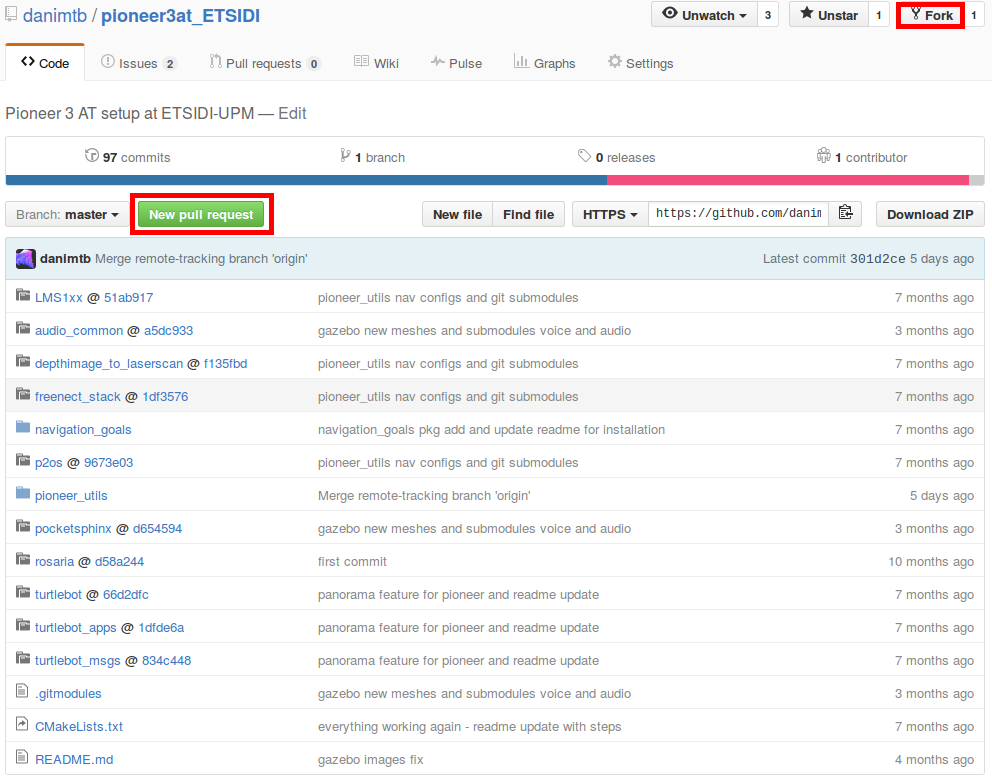
\includegraphics[width=0.8\textwidth]{figuras/pioneer3at_ETSIDI.png}
\caption{Vista del repositorio de GitHub de este proyecto.}
\label{fig:pioneer3at_ETDSIDI}
\end{figure}

De esta forma podemos guardar los cambios realizados en el repositorio de la persona que hace la modificaci�n, con la intenci�n de incorporar los cambios m�s tarde al repositorio de desarrollo principal (\url{https://github.com/danimtb/pioneer3at_ETSIDI.git}) mediante Pull Request.

\subsection{Gesti�n de las dependencias}

 ROS se vale de la informaci�n almacenada en la definici�n de cada uno de sus paquetes en \textit{package.xml} y gestionar algunas dependencias de librer�as, para lo cual se sirve de la herramienta rosdep **referencia** creada por los desarrolladores de ROS para este prop�sito.

Para comenzar a utilizarla inicializamos rosdep y actualizamos las dependencias:

\begin{code}[htp]
\begin{lstlisting}[style=consola]
$ sudo rosdep init
$ rosdep update
\end{lstlisting}
\caption{Inicializando la herramienta \textit{rosdep}.}
\end{code}

A continuaci�n se describen los pasos necesarios para instalar las dependencias de cada secci�n:

\begin{itemize}
\item Navegaci�n: Instalamos los paquetes adicionales para realizar la navegaci�n y mapeo (Cap�tulo \ref{chapter:navegacion}).
\end{itemize}

\begin{code}[!htp]
\begin{lstlisting}[style=consola]
$ sudo apt-get install ros-indigo-navigation
$ sudo apt-get install ros-indigo-gmapping
\end{lstlisting}
\caption{Instalando los paquetes de navegaci�n mapeo.}
\end{code}

\begin{itemize}
\item Rosaria: Instalamos las dependencias de RosAria, principalmente la librer�a Aria.
\end{itemize}

\begin{code}[!htp]
\begin{lstlisting}[style=consola]
$ rosdep install rosaria
\end{lstlisting}
\caption{Instalando las dependencias de rosaria.}
\end{code}


Para el reconocimiento de los comandos de voz utilizamos el paquete \textit{pocketsphinx}:

\begin{itemize}
\item pocketsphinx: Instalamos los paquetes de conversion a texto y buscamos las dependencias del paquete.
\end{itemize}

\begin{code}[!htp]
\begin{lstlisting}[style=consola]
$ sudo apt-get install gstreamer0.10-gconf
$ rosdep install pocketsphinx
\end{lstlisting}
\caption{Instalando las dependencias de \textit{pocketsphinx} y \textit{gstreamer}.}
\end{code}

Es posible que necesitemos las dependencias a�adidar de \textit{audio\_capture}.

\begin{code}[!htp]
\begin{lstlisting}[style=consola]
$ rosdep install audio_capture
\end{lstlisting}
\caption{Instalando las dependencias de \textit{audio\_capture}.}
\end{code}

Para el audio (sintetizado de voz) utilizamos el nodo \textit{sound\_play}, por lo que debemos instalar sus dependencias.

\begin{itemize}
\item sound\_play: Nodo para el sintetizado de voz y reproducir sonidos.
\end{itemize}

\begin{code}[!htp]
\begin{lstlisting}[style=consola]
$ rosdep install sound_play
\end{lstlisting}
\caption{Instalando las dependencias de \textit{sound\_play}.}
\end{code}

Una vez disponemos de todos los paquetes y sus respectivas dependencias no debemos olvidarnos de que es necesario compilarlos:

\begin{code}[!htp]
\begin{lstlisting}[style=consola]
$ cd ~/catkin_ws
$ catkin_make
\end{lstlisting}
\caption{Compilando los paquetes del espacio de trabajo Catkin.}
\end{code}


\section{Configuraci�n del hardware}

En este ap�ndice se describen algunos ajustes �tiles del hardware que se ha utilizado en el proyecto. Esta informaci�n es importante para que el sistema rob�tico desarrollado funcione pero no ha sido incluida dentro del cuerpo de la memoria para no alargar las explicaciones.

En cualquier caso, los procemientos que a continuaci�n se describen es probable que no sea necesarioz volver a realizarlos en futuros usos del robot si se mantiene la configuraci�n descrita en este trabajo.

\subsection{Calibraci�n de la odometr�a}\label{subsection:odometria}
La lectura de la posici�n de los motores del robot se realiza mediante unos encoders situados en el eje de cada motor.

El firmware ARCOS de la placa controladora del robot es actualizable y gestiona os par�metros de calibraci�n de la odometr�a. Este firmware es actualizable aunque para ello es necesario ponerse en contacto con el fabricante Adept.

Estos par�metros referentes a la odometr�a son configurables a trav�s de la librer�a Aria en caso de que no se desee acceder a modificar el firmware del robot.

Los par�metros a considerar son los siguientes:

\begin{itemize}
\item TicksMM
\item DriftFactor
\item RevCount
\end{itemize}

El nodo de ROS RosAria es capaz de pasar estos par�metros a la placa controladora del robot a trav�s de Aria. Es por ello que podemos configurar din�micamente estos par�metros del robot cada vez que ejecutamos el nodo. De esta forma evitamos tener que recurrir a Adept y a software espec�fico para modificar los par�metros de ARCOS.

Podemos ver la descripci�n de estos par�metros en el manual del robot Pioneer 3 AT **referencia**

**IMAGEN DEL MANUAL**

EL procedimiento para calcular cada uno de estos par�metros es el siguiente:



\subsection{Ordenador de abordo Intel NUC}

\subsection{Sensor Kinect}
El sensor Kinect utilizado en el proyecto no dispone de ninguna moficiaci�n espec�fica o modo de funcionamiento especial. Lo referente a su conexionado ha sido descrito anteriormente en la secci�n \label{subsection:implementacion_kinect}.

Tan solo indicar que puede realizarse una primera toma de contacto a trav�s de la librer�a \textit{libfreenect}. Una manera r�pida de hacerlo es utilizando el gestor de depencencias en C++ biicode **LINK A BIICODE**, en un sistema operativo Ubuntu siguiendo esta gu�a **URL DE BIICODE**.

\subsection{L�ser SICK LMS100}\label{subsection:sicklms100_apendice}

El sensor l�ser LMS100 de la marca Sick es un sensor de ampli rango y largo alcance de tipo industrial.

El fabricante Sick ofrece un software propietario llamado SOPAS Ingineering Tool que permite acceder a la configuraci�n interna del sensor. Este software tan solo puede utilizarse bajo el sistema operativo Microsoft Windows, en concreto ha sido utilizado con Windows 7.

Para instalarlo hay que recurrir a la web del fabricante: \url{https://www.mysick.com/eCat.aspx?go=FinderSearch&Cat=Row&At=Fa&Cult=English&FamilyID=235&Category=Software&Selections=54195,54293}

Para configurar el dispositivo debemos enchufarlo a un puerto Ethernet de un ordenador con el software instalado y proporcionarle alimentaci�n.

El puerto ethernet del ordenador debe estar configurado para obtener una IP autom�tica. Una vez aparezca la red como conectada procedemos a abrir el software SOPAS.

\begin{figure}[!htp]
\centering
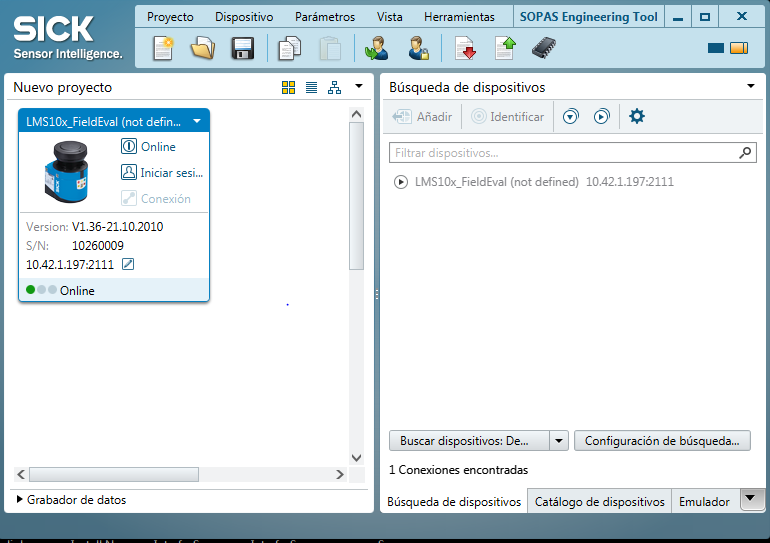
\includegraphics[width=0.8\textwidth]{figuras/sopas1.png}
\caption{Software Sick SOPAS con el sensor detectado.}
\label{fig:sopas1}
\end{figure}

Autom�ticamente detectar� el dispositivo pero seguramente no podamos acceder a �l debido a una direcci�n IP err�nea.

Para ello abriremos el apartado de configuraci�n y selecionamos ''Asignar IP autom�ticamente" para que nos asigne el rango adecuado.

\begin{figure}[!htp]
\centering
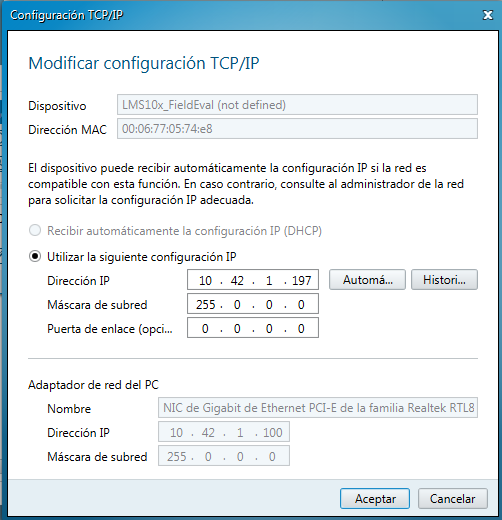
\includegraphics[width=0.8\textwidth]{figuras/sopas2.png}
\caption{Configurando la direcci�n IP del dispositivo.}
\label{fig:sopas2}
\end{figure}

Si queremos una direcci�n IP de determinado rango, la mejor manera de proceder es asignar al adaptador de red del ordenador una IP manual del rango deseado y realizar el procedimiento anterior.

Tambi�n podemos acceder a los par�metros del sensor y visualizar en un gr�fico la informaci�n que est� captando en el momento.

\begin{figure}[!htp]
\centering
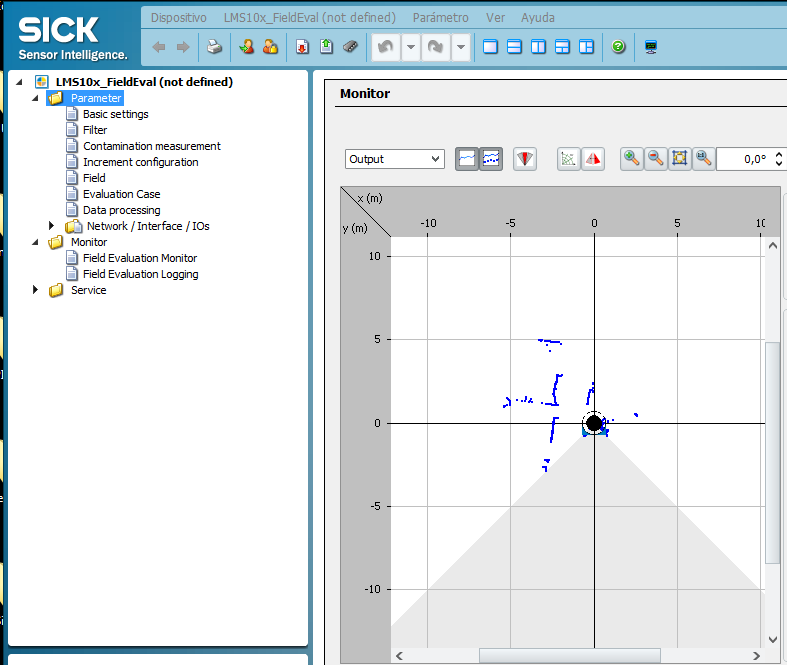
\includegraphics[width=0.8\textwidth]{figuras/sopas3.png}
\caption{Gr�fico de la informaci�n captada por el sensor en el software SOPAS.}
\label{fig:sopas3}
\end{figure}

A partir de aqu� podremos conectarnos al l�ser con el nodo ROS LMS1xx, configurando una IP fija en el adaptador de red ethernet del ordenador al que lo conectemos, en este caso el ordenador Intel NUC del robot.

\begin{itemize}
\item Direcci�n IP del l�ser Sick LMS100:
\item Direcci�n IP del adaptador ethernet del ordenador Intel NUC: 
\end{itemize}

Para m�s informaci�n conviene leer el manual que ofrece Sick \cite{sicklms100}.

\chapter{Manual de uso del robot}
Este ap�ndice es una gu�a de funcionamiento del robot Pioneer 3 AT (Petrois) utilizado e implementado al acabar este proyecto fin de grado.

\section{Encendido del robot}
El robot se enciende mediante un interruptor situado en su parte trasera, el cual proporciona alimentaci�n general a todos los sistemas.

Adicionalmente es necesario encender el ordenador de abordo Intel NUC mediante su correspondiente bot�n y el altavoz frontal del robot, para lo cual ser� necesario tener activada la alimentaci�n auxiliar 2 (AUX 2) en el panel de control.

**DESCRIPCION ENCENDIDO INTEL NUC**

\section{Panel de control y parada de emergencia}
El panel de control del robot se sit�a en su lateral derecho. Aqu� disponemos de una serie de botones, indicadores luminosos, ac�sticos y conexiones.

\begin{figure}[!htp]
\centering
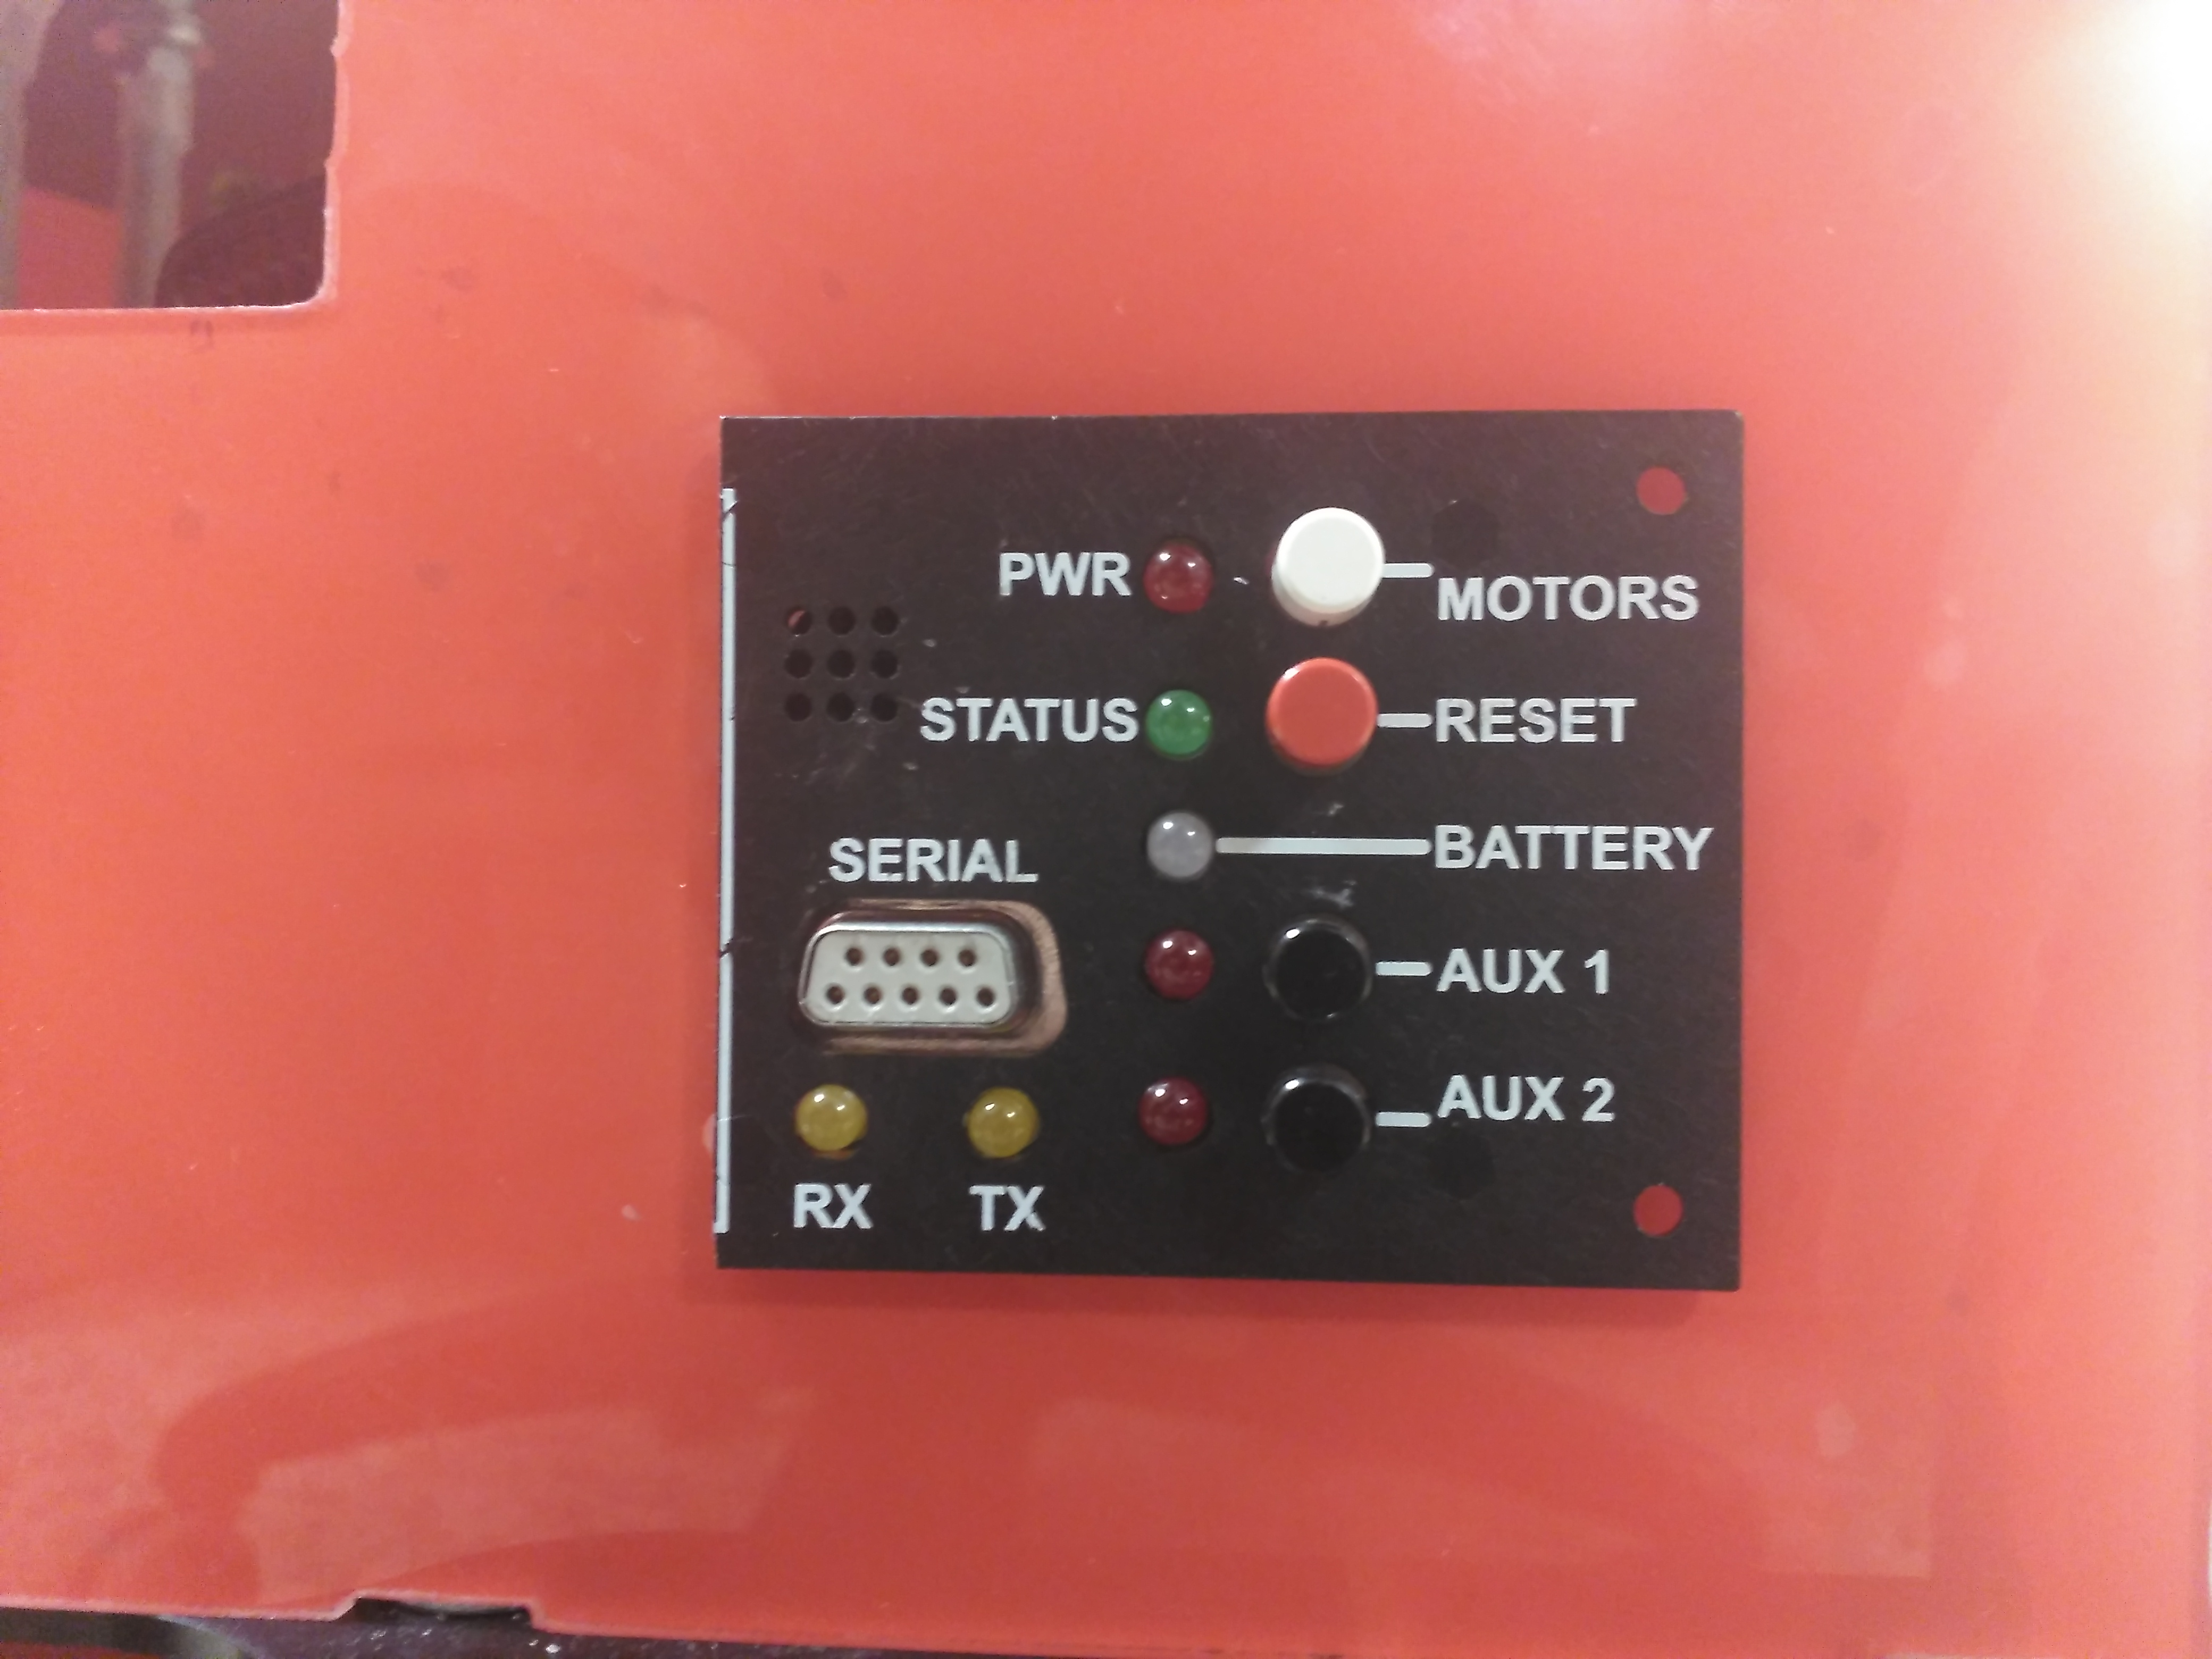
\includegraphics[width=0.6\textwidth]{figuras/panel_derecho.jpg}
\caption{Panel de control del robot Petrois.}
\label{fig:panel_derecho}
\end{figure}

A continuaci�n se describe cada uno de los elementos de la figura \ref{fig:panel_derecho}:
\begin{itemize}
\item Pulsador MOTORS: Encargado de habilitar y deshabilitar los motores del robot. La activaci�n de los mismos puede realizarse a trav�s de software. Es necesario pulsar este bot�n para rearmar el robot cuando se pulsa la seta de emergencia. Si se pulsa una vez m�s el robot realiza una secuencia de movimientos para comprobar que los motores funcionan correctamente.
\item Pulsador RESET: Resetea la placa controladora del robot. El robot queda su estado inicial, tal y como si lo acab�semos de encender. Al pulsar este bot�n se interrumpe cualquier comunicaci�n con la placa de control.
\item Pulsador AUX 1: Habilita la alimentaci�n 1 de la placa de alimentaci�n. No se encuentra en uso.
\item Pulsador AUX 2: Habilita la alimentaci�n 2 de la placa de alimentaci�n. Es necesario tenerlo habilitado para que el altavoz frontal del robot funcione.
\item LED PWR: Indica el estado de los motores.
\item LED STATUS: Indica el estado del robot.
\item LED BATERY: Indica el estado de carga de la bater�a.
\item LEDs AUX 1 y AUX 2: Indica si las alimentaciones auxiliares se encuentran activas.
\item LEDs RX y TX: Muestran el estado de la comunicaci�n con la placa de control.
\item SERIAL: Puerto RS-232 que comunica con la placa de control. Puede ser utilizado para conectar un ordeandor externo directamente la placa de control del robot.
\end{itemize}

Muchos de los estados anteriores se indican mediante una se�al ac�stica. El reseteo de la placa tiene un sonido caracter�stico al igual que cuando se pierde la conexi�n con la placa de control.

El pulsador de emergencia se encuentra en la parte superior del robot y es de vital importancia cuando el robot se mueve de manera descontrolada, choca o est� en peligro la integridad de una persona o del propio robot. Es por ello que se recomienda su uso siempre que se encuentre en una situaci�n de las anteriores.

\begin{figure}[!htp]
\centering
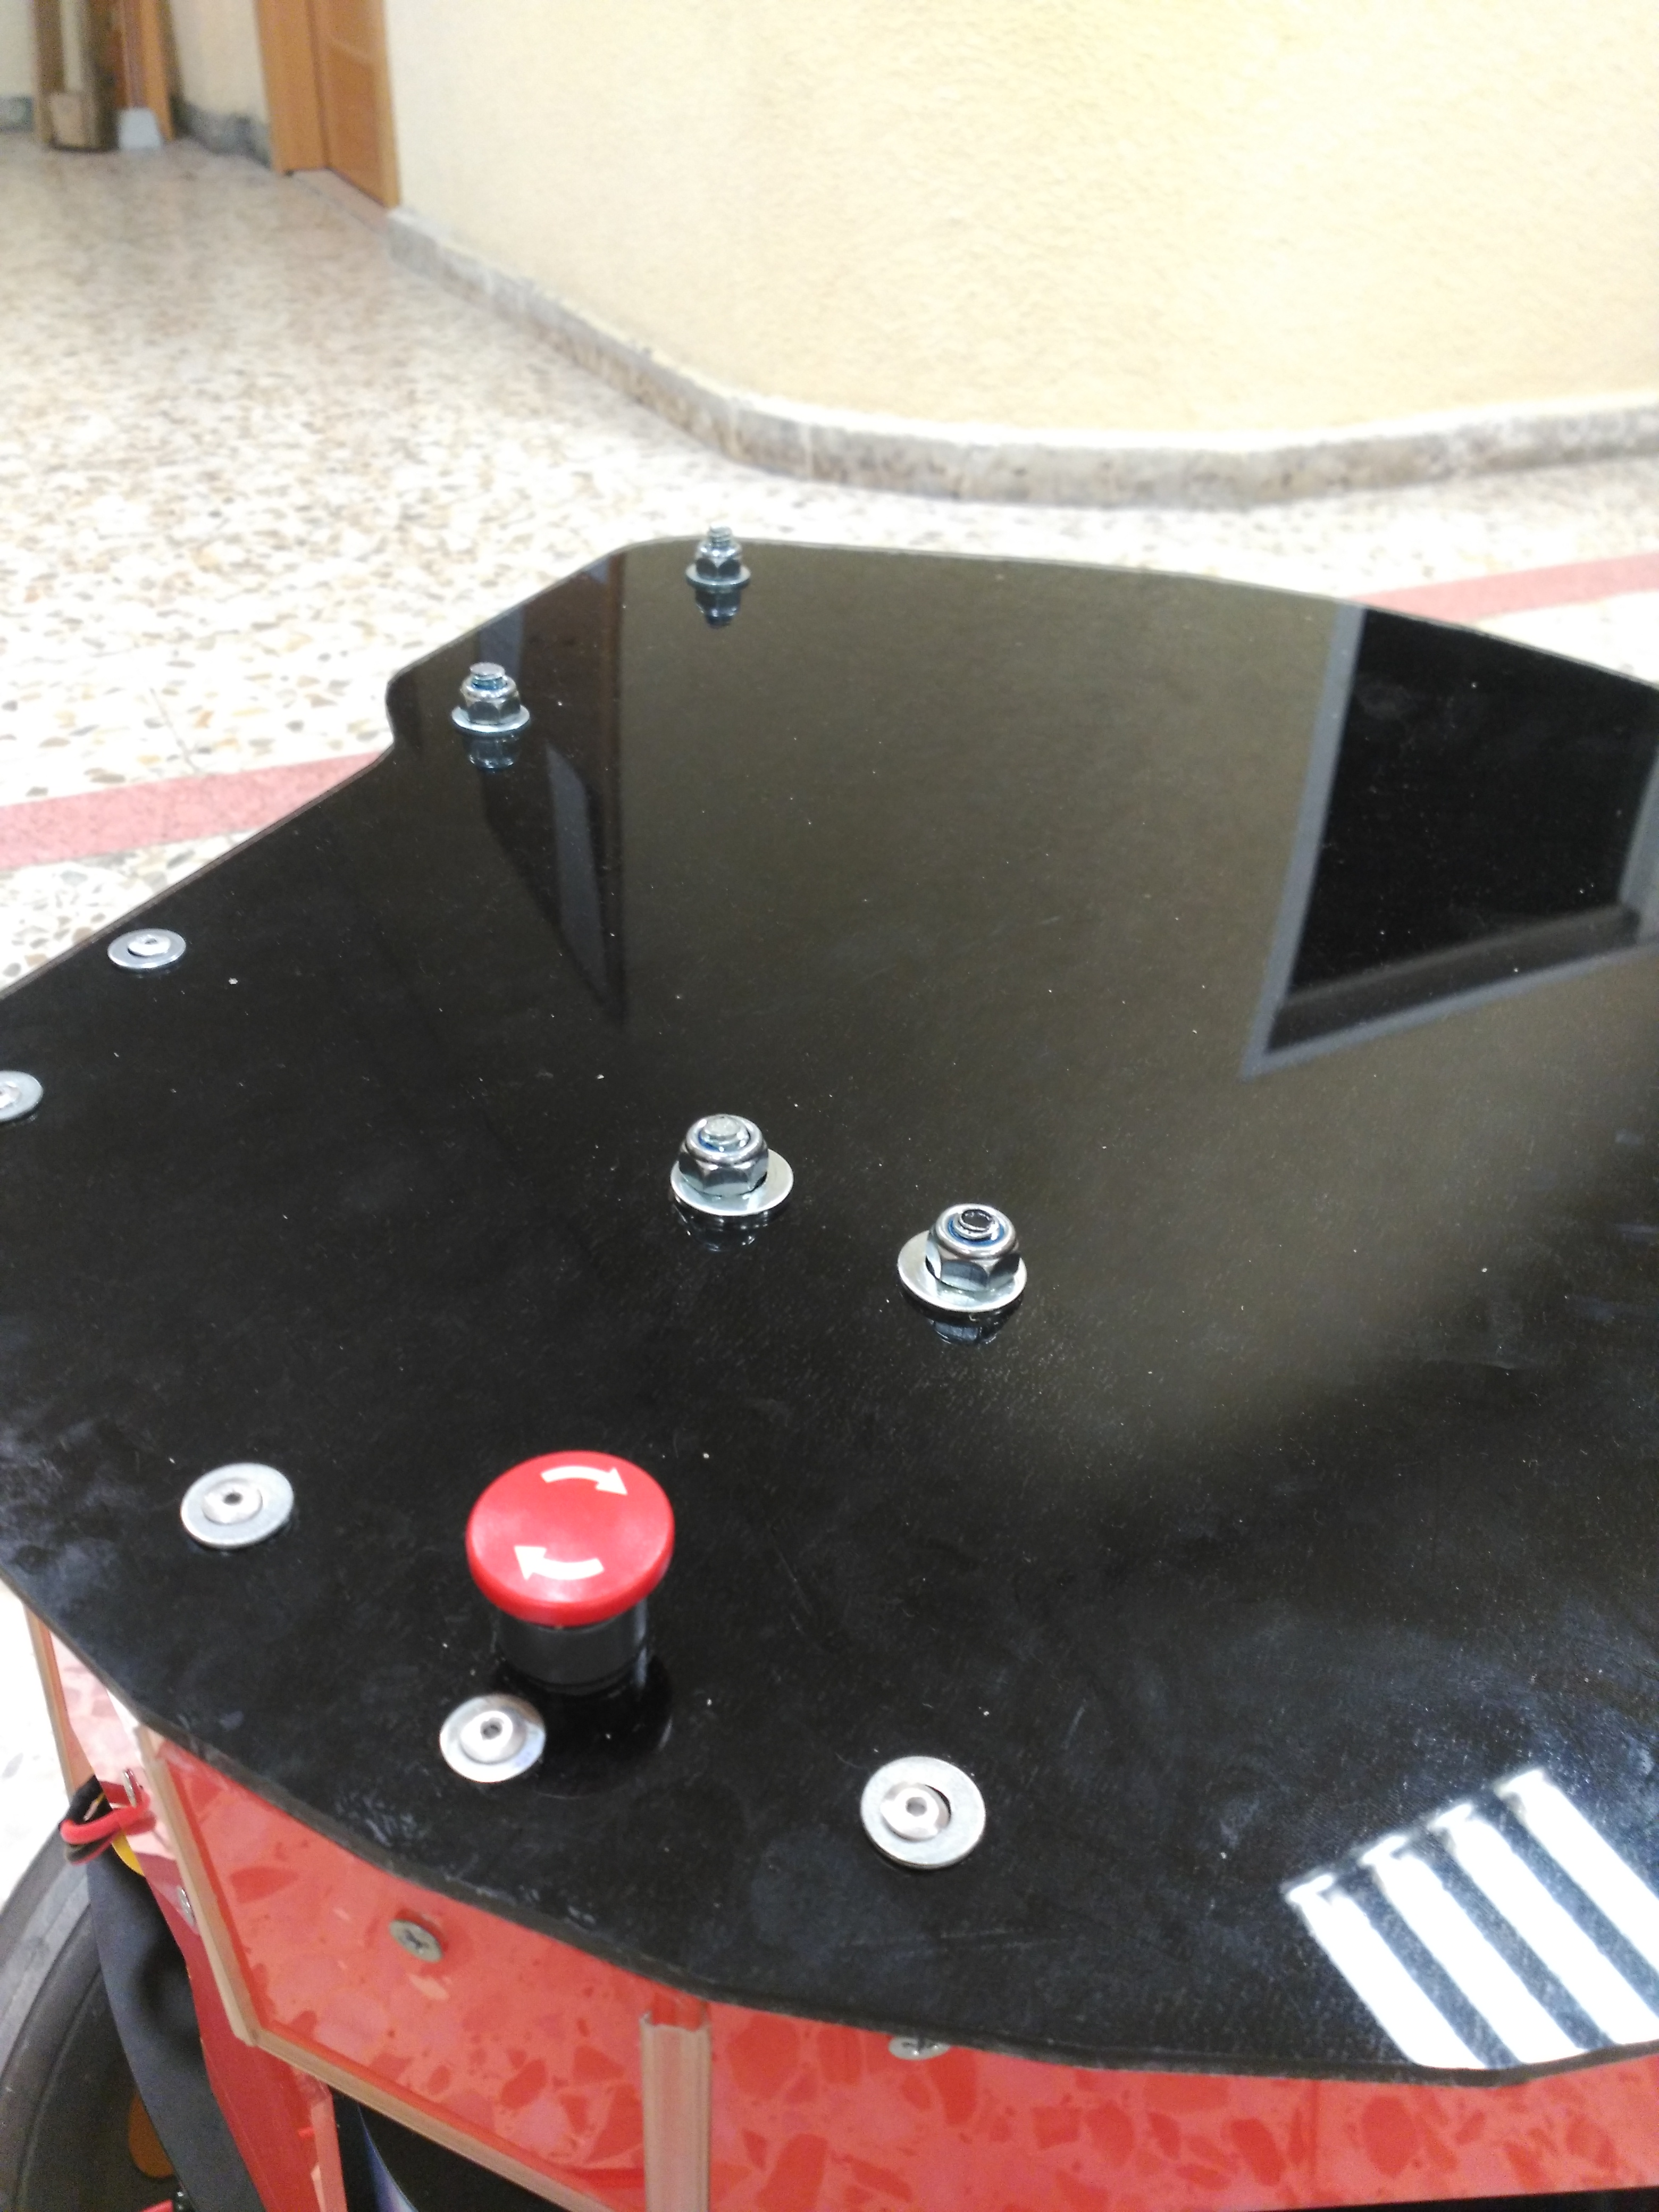
\includegraphics[width=0.5\textwidth]{figuras/seta_emergencia.png}
\caption{Bot�n de parada de emergencia del robot Petrois.}
\label{fig:seta_emergencia}
\end{figure}

Al pulsar la seta de emergencia �sta quedar� enclavada y el robot dar� una se�al ac�stica continuada indicando que se encuentra en parada. En este punto los motores quedan deshabilitados y las ruedas del robot pueden moverse libremente.

Para rearmar el robot basta con devolver la seta de emergencia a su posici�n DE reposo girando levemente la misma en el sentido de las flechas. Despu�s es necesario pulsar el bot�n MOTORS para volver a habilitar los motores.

Cabe indicar que la comunicaci�n de cualquier ordenador con la placa de control del robot no se interrumpe, por lo que al rearmar el robot es posible que �ste contin�e con los movimientos previos a la parada de emergencia. Aseg�rese de que las consignas de movimiento son las correctas y ponga especial precauci�n cuando realice el rearmado del robot.

Para informaci�n m�s extensa y detallada se recomienda leer la gu�a de usuario ofrecida por el fabricante **REFERENCIA**.

\section{Conexi�n mediante un ordenador externo v�a Wifi}

Al encender el ordenador Intel NUC, �ste est� configurado para generar directamente un HotSpot Wifi o red Ad-hoc con el nombre "P3AT". Esta red Wifi maneja direcciones IP en el rango 10.42.0.X por lo que es recomendable conectarse a ella con una IP fija que est� dentro de ese rango. SU contrase�a es "pioneer3at"

Si se est� ejecutando el nodo MASTER en el ordenador Intel NUC, �ste estar� configurado con la IP 10.42.0.1. Para indicar que queremos conectarnos a un nodo MASTER que se ejecuta en otra m�quina debemos editar el script \textit{.bashrc} del ordenador externo, que se ejecuta siempre que abrimos una terminal.

Para editarlo, abrimos la terminal y escribimos:

\begin{code}[htp]
\begin{lstlisting}[style=consola]
$ gedit ~/.bashrc
\end{lstlisting}
\caption{Abriendo el \textit{.bashrc}.}
\end{code}

Una vez abierto, al final del archivo a�adimos las siguientes dos l�neas:

\begin{code}[htp]
\begin{lstlisting}[style=consola]
export ROS_IP=10.42.0.77
export ROS_MASTER_URI=http://10.42.0.1:11311
\end{lstlisting}
\caption{A�adidendo las direcciones IP al \textit{.bashrc}.}
\end{code}

La primera l�nea indica la IP fija con la que el ordenador externo se conecta a la red Ad-hoc del Intel NUC. Modificar la IP y escribir la IP del ordeandor externo.
La direcci�n IP del MASTER es la direcci�n que est� configurada en el Intel NUC y a la que tratar�n de conectarse los nodos cuando se lancen desde el ordenador externo.

Este procedimiento est� hecho igual en el Intel NUC pero indicando tan solo que la IP de ese equipo es \textbf{ROS\_IP=10.42.0.77}.

\section{Acceder a la placa de alimentaci�n}

La placa de alimentaci�n se encuentra bajo la tapa negra principal del robot, justo debajo del sensor Kinect.

Su posici�n no es muy accesible y se recomienda encarecidamente leer el manual para tener acceso a la misma.

Por otro lado, siempre puede acderse a la alimetaci�n de 12 voltios a trav�s del cable de alimentaci�n del sensor Kinect y a 5 voltios a trav�s de los cables de alimentaci�n del altavoz delantero.

\section{Cargar las bater�as del robot}
El robot Pioneer 3 AT dispone de un pack de 3 bater�as est�ncas de plomo-�cido a 12 voltios. Estas bater�as suministran alimentaci�n a todos los sistemas del robot y proporcionan una autonom�a aproximada de 2 horas de funcionamiento.

El acceso a las bater�as se encuentra en el interior del chasis del robot y son accesibles mediante una trampilla trasera.

**IMAGEN**

La carga de las bater�as se realiza con el adaptador de la figura **TAL** a trav�s del conector de carga situado junto al interruptor de alimentaci�n general.

\begin{figure}[!htp]
\centering
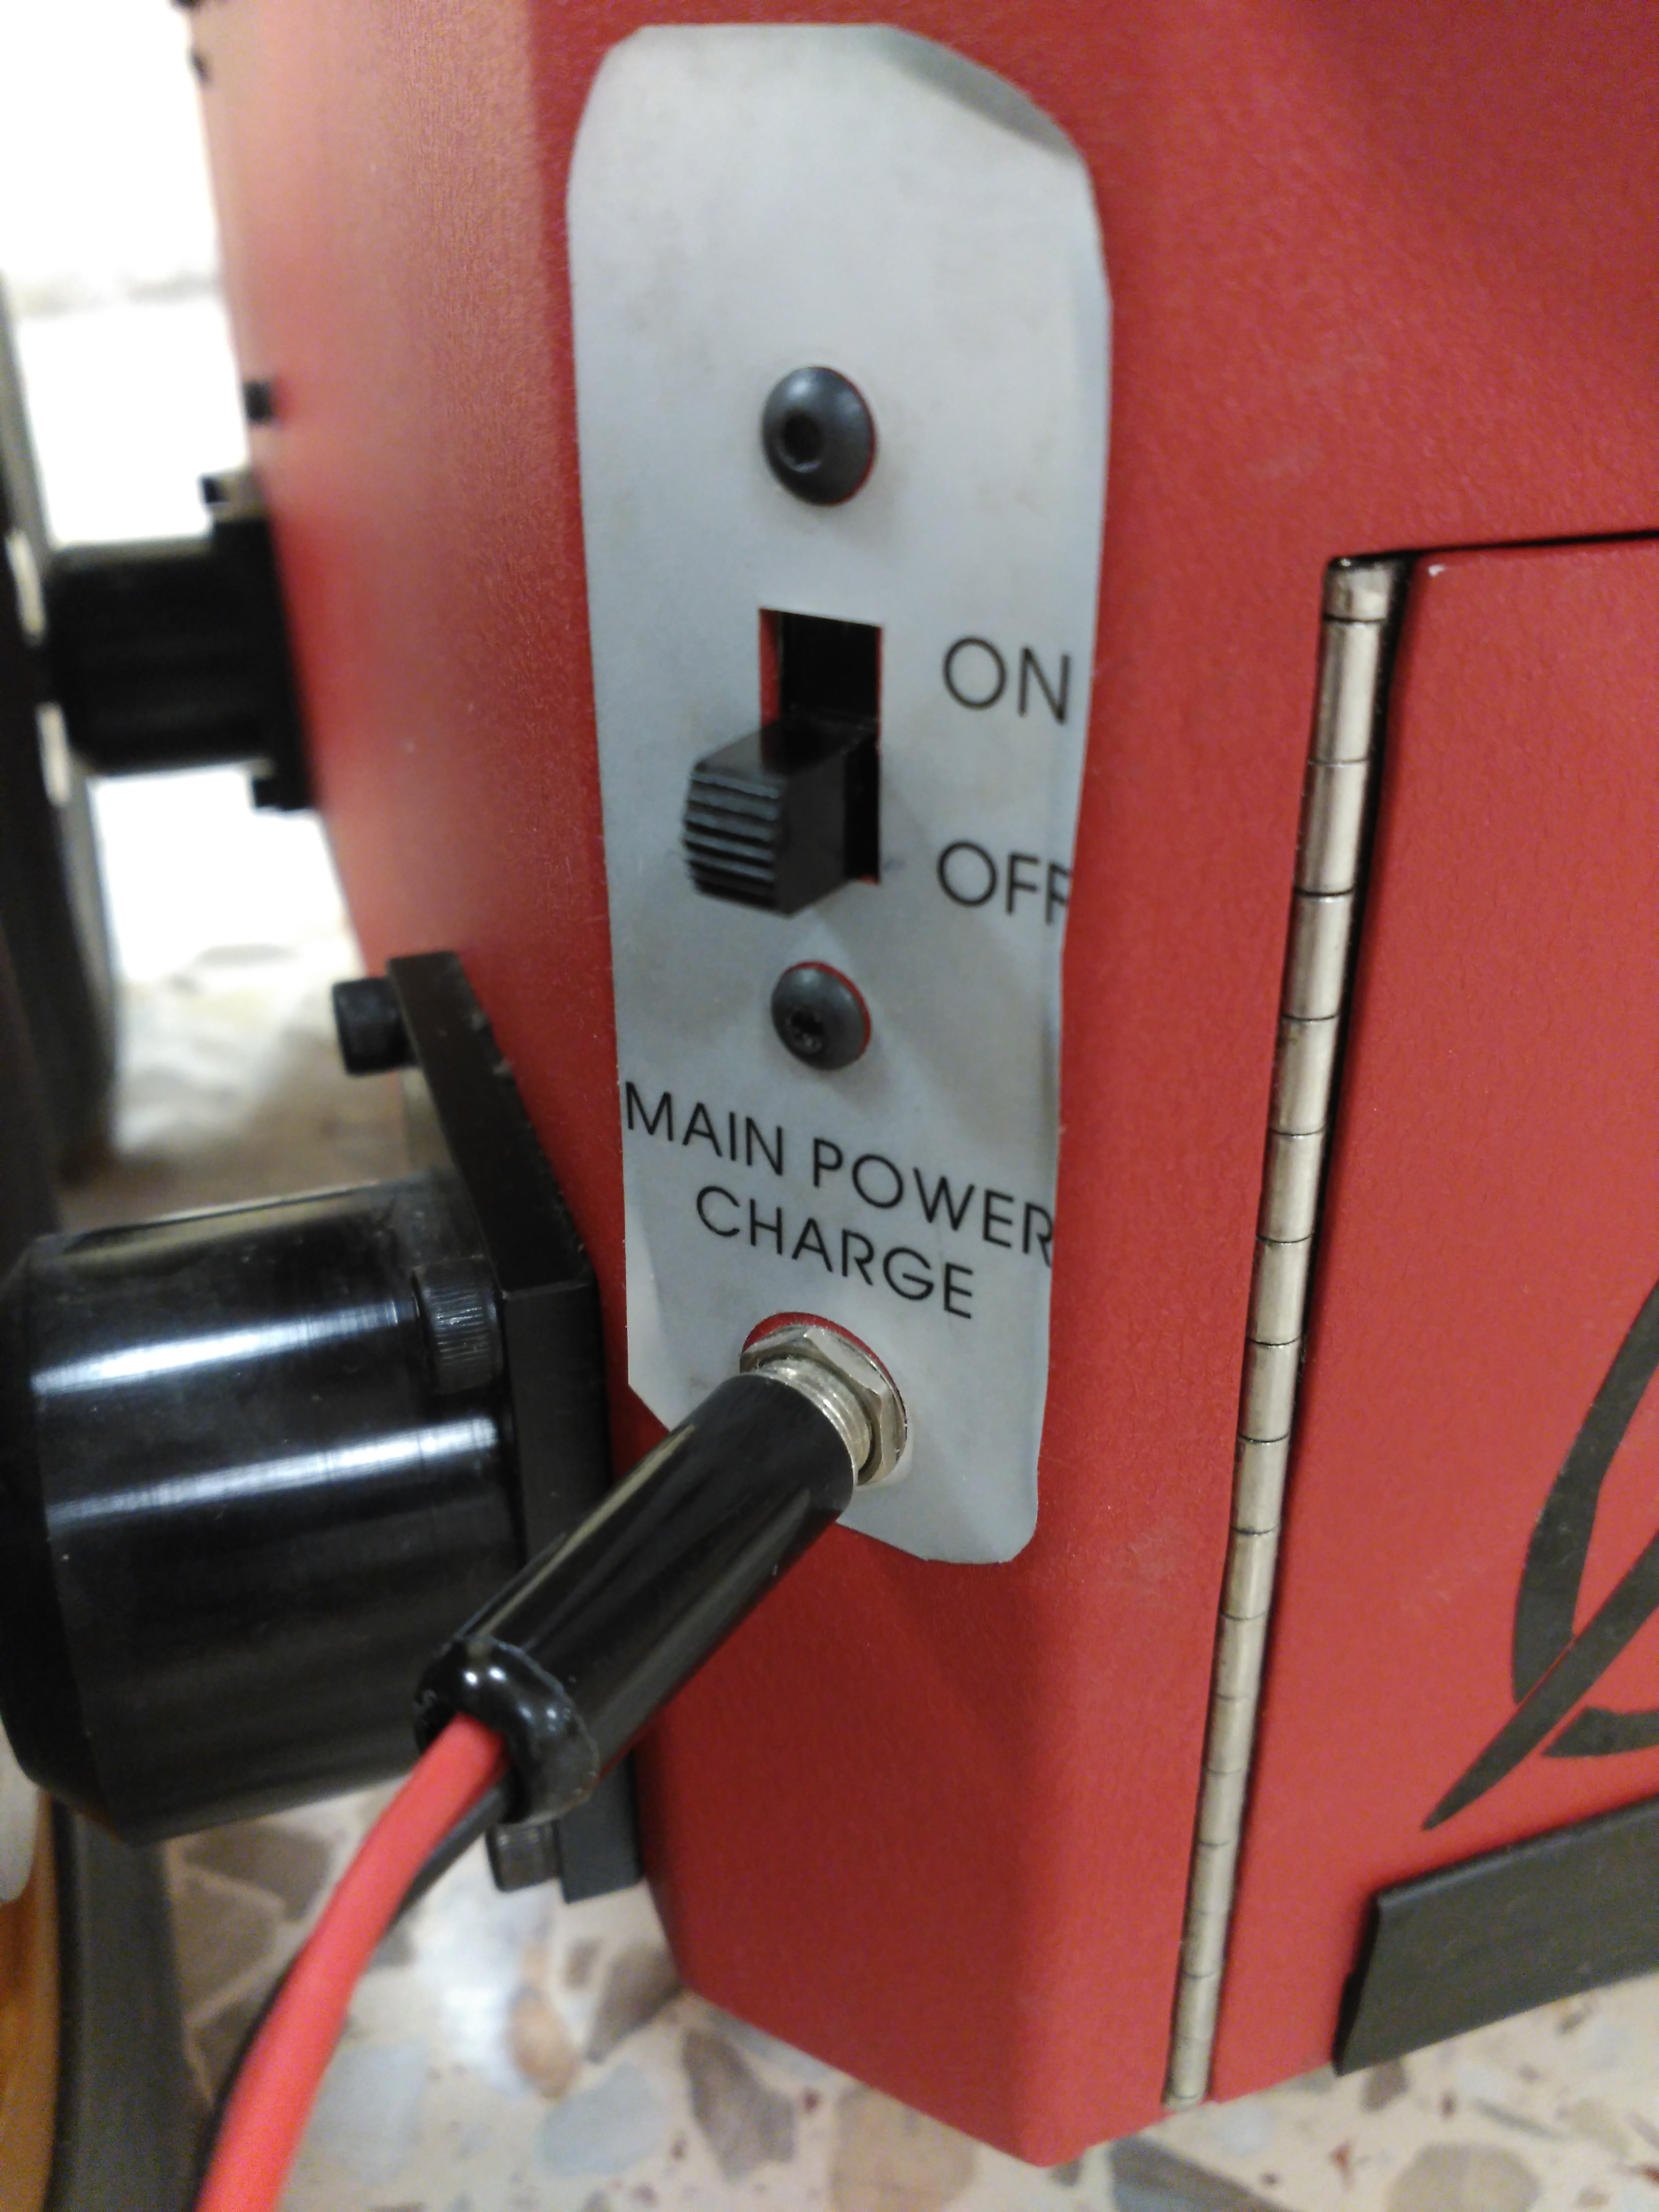
\includegraphics[width=0.45\textwidth]{figuras/puerto_carga.jpg}
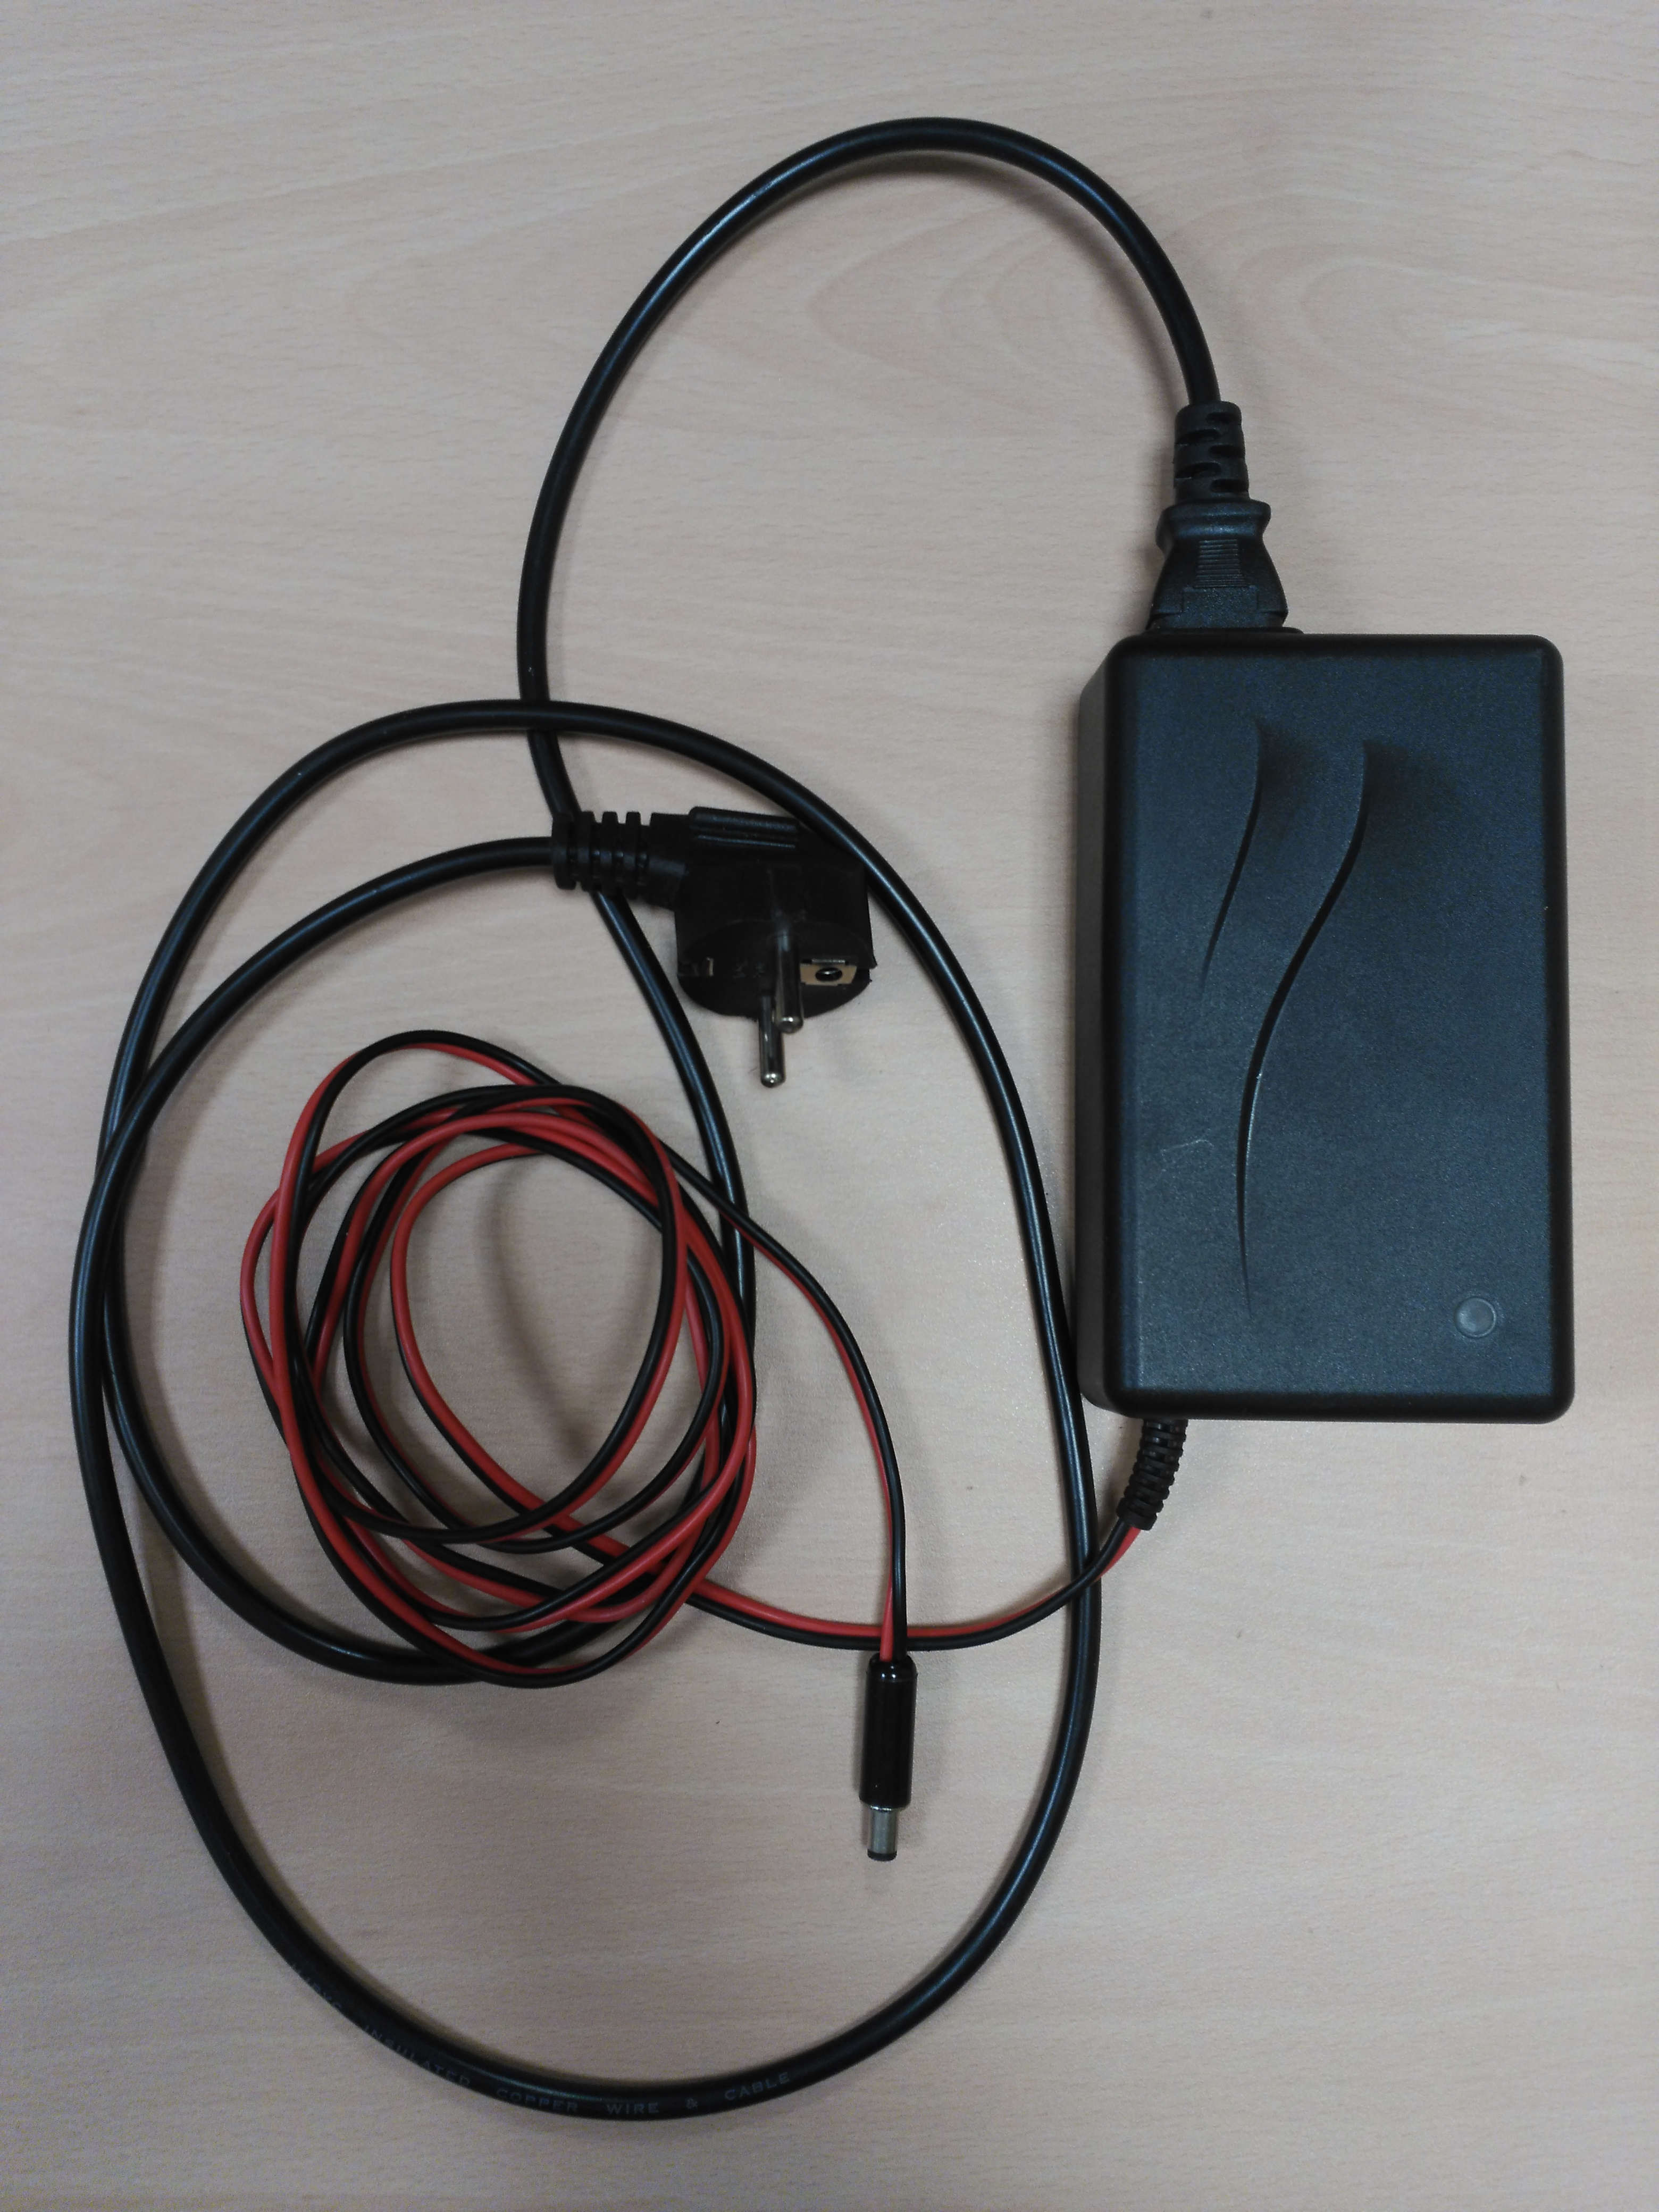
\includegraphics[width=0.45\textwidth]{figuras/cargador.jpg}
\caption{Puerto de carga y cargador del robot Petrois.}
\label{fig:seta_emergencia}
\end{figure}

No ha podido estimarse el tiempo de carga completo, sin embargo el propio cargador incorpora un indicador luminoso que muestra el estado de carga de las bater�as.

\section{Ordenador interno del Pioneer 3 AT}

EL ordenador interno del robot Pioneer 3 AT se encuentra en desuso.

Todos los controles necesarios para acceder al ordenador est�n disponibles a trav�s del panel situado en el lateral izquierdo del robot.

\begin{figure}[!htp]
\centering
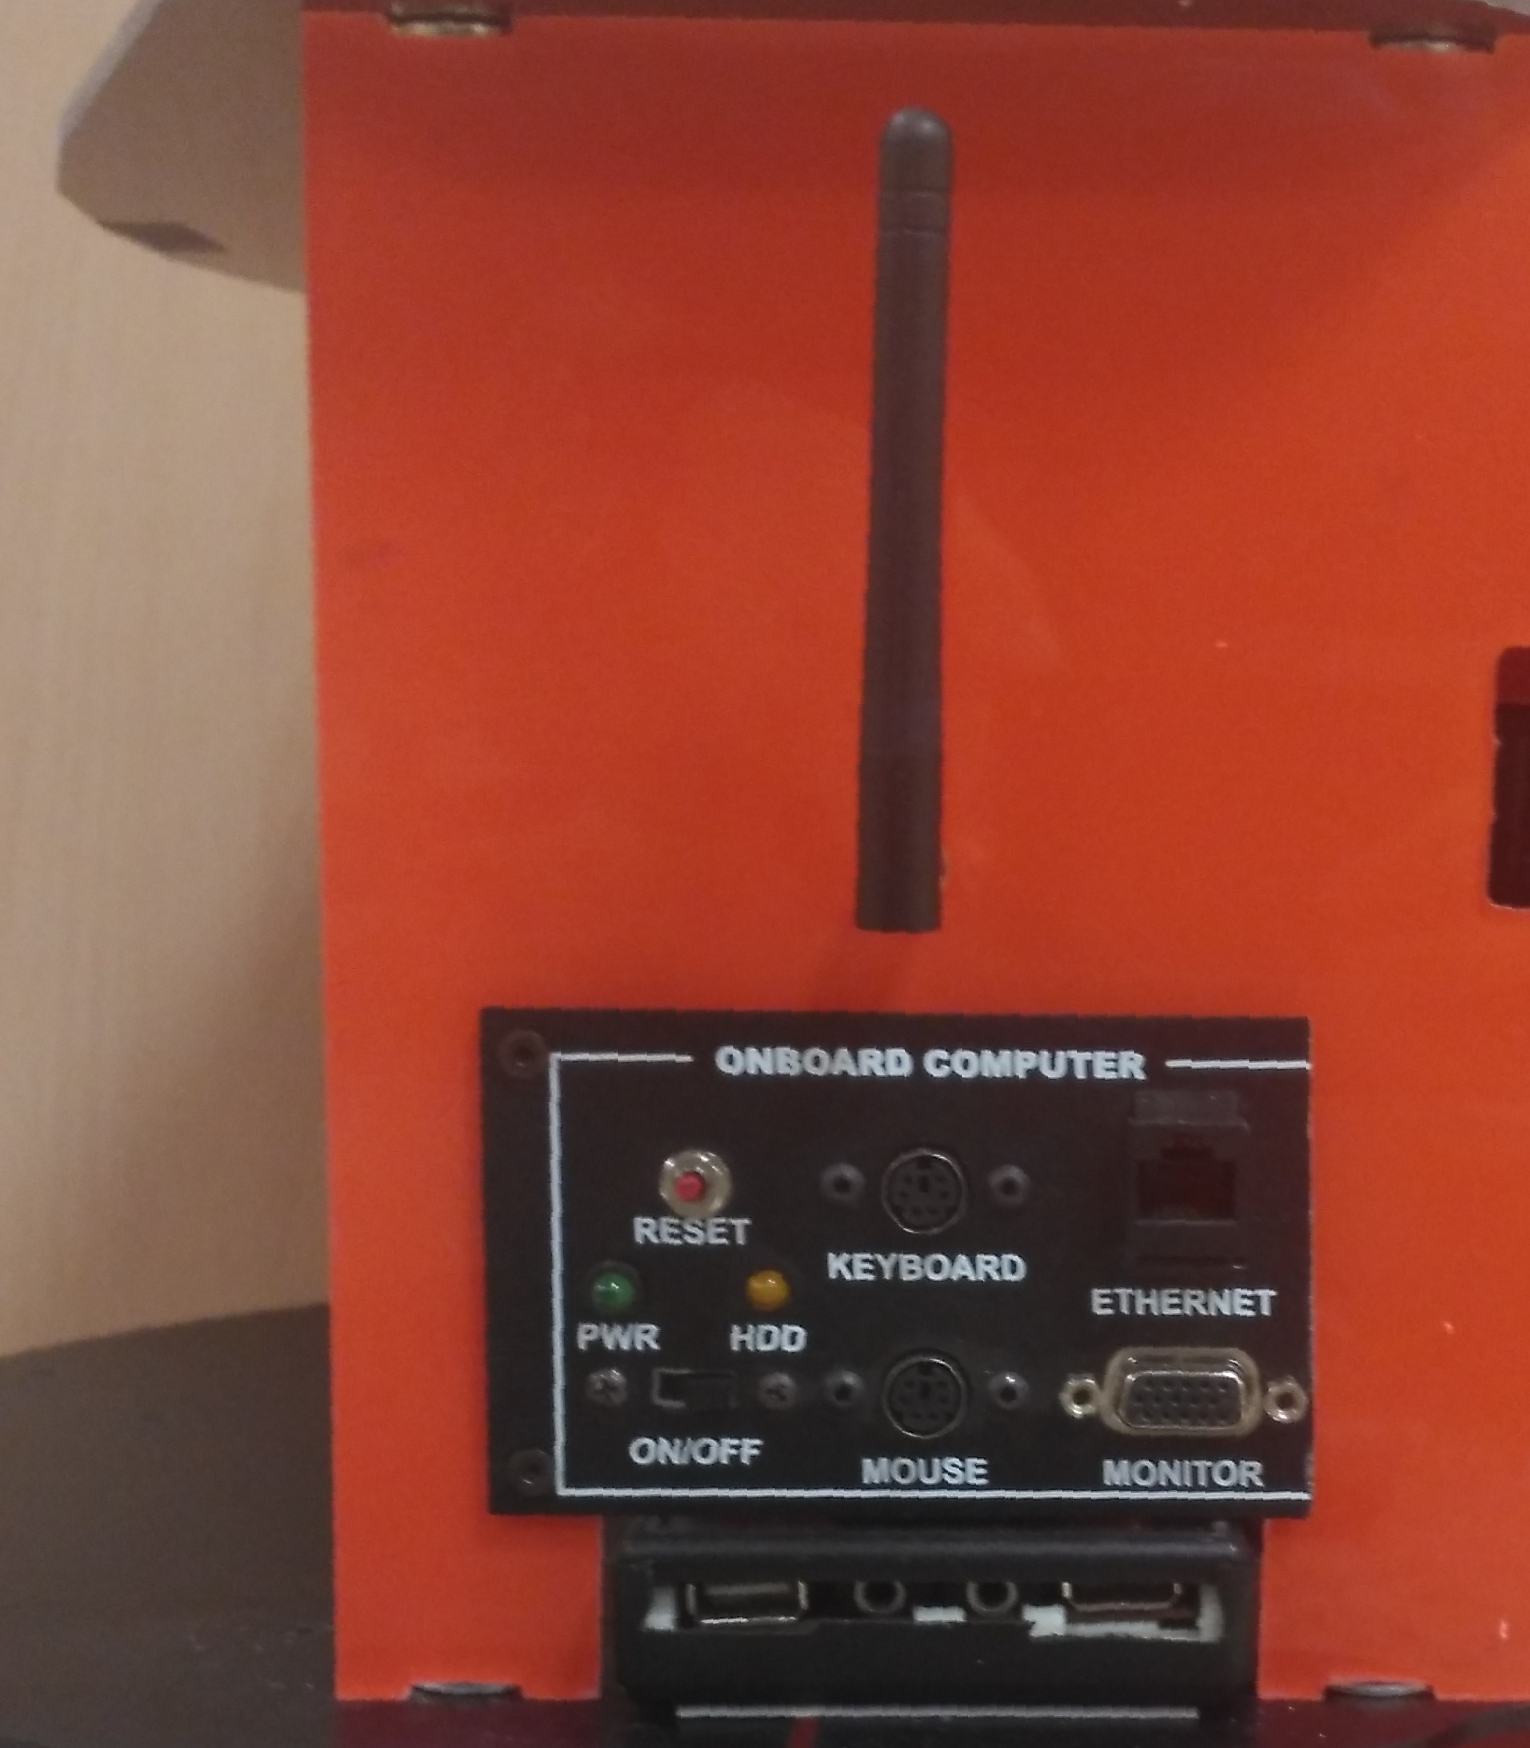
\includegraphics[width=0.5\textwidth]{figuras/panel_izquierdo.png}
\caption{Panel del ordenador interno (lateral izquierdo) del robot Petrois.}
\label{fig:panel_izquierdo}
\end{figure}

En este lateral encontramos elementos adicionales como la antena de conexi�n wifi del ordenador interno y el acceso a los puertos USB y Jacks de micr�fono y auriculares.

\textbf{IMPORTANTE:}\\
Originalmente este ordenador se encontraba conectado a la placa controladora del robot de manera interna a trav�s el puerto COM1 (Accesible en el interior del robot). En su lugar se conect� el convertidor de RS-232 a USB utilizado con el ordeandor Intel NUC, por lo que el ordenador interno se encuentra desconectado del robot.

\textbf{IMPORTANTE:}\\
Uno de los ventiladores internos situado en la parte frontal derecha del robot fue desconectado debido a su elevado ruido y su encendido permanente. En caso de utilizar el ordenador interno del robot es posible que sea necesario volver a conectarlo. Sin embargo no existe riesgo de sobrecaentamiento ya que el propio ordenador dispone de un ventilador adicional que se pone en marcha al encencerlo.


\chapter{Informaci�n y documentos ONLINE}
 En este ap�ndice se muestra informaci�n adicional de todo tipo referente al proyecto y a los materiales utilizados.

\section{Repositorio de c�digo}
Como se ha descrito anteriormente, el repositorio de c�digo desarrollado en ente proyecto se encuentra almacenado en GitHub. Puede consultarse su linea de tiempos, commits e incluso realizar preguntas en el apartado de Issues.

\url{https://github.com/danimtb/pioneer3at_ETSIDI}

**Im�gen del repositorio**

En �l podr� encontrar una peque�a gu�a \textit{Readme} actualizada con informaci�n sobre las utilidades que ofrece el repositorio y en concreto el desarrollo realizado en el paquete \textit{pioneer\_utils}, donde se encuentra la mayor�a del desarrollo.

\subsection{Readme}
Copia del documento \textit{Readme} del repositiorio.

**COPIA**

\section{Preguntas en ROS Answers y Github}
Pregunta del l�ser
Preguntal del Intel Nuc

Issue cleapath robotics

\section{Multimedia}
Colecci�n de v�deos:

\begin{itemize}
\item V�deos de este proyecto:
\item V�deos de antiguos proyectos:
\end{itemize}

Im�genes:
\begin{itemize}
\item Im�genes de este proyecto:
\item Im�genes de antiguos proyectos:
\end{itemize}

\section{Memoria del trabajo}

La memoria del trabajo ha sido desarrollada en \LaTeX, bajo el editor \textit{TexStudio} en un ordenador con sistema operativo GNU/Linux Ubuntu 14.04 LTS.

Su desarrollo ha sido puesto bajo un controlador de versiones y alojado en el siguiente repositorio de github:

\url{https://github.com/danimtb/TFG_pioneer3at}

En el propio repositorio se encuentran las figuras utilizadas y los archivos .tex, donde se ha escrito el mismo,  y la bibligraf�a empleada.

El documento PDF compilado de \LaTeX puede consultarse en el siguiente enlace:

\url{https://github.com/danimtb/TFG_pioneer3at/TFG.pdf}
%genera doble hoja en blanco
\cleardoublepage
%se incluye la bibliograf�a. Archivo de tipo .bib (bibtex)
\bibliographystyle{alpha}
\bibliography{bibliografia/bibliografia}

\backmatter

%fin del documento
\end{document}
